\documentclass[a4paper,11pt]{memoir}
\maxsecnumdepth{subsection} 
\setsecnumdepth{subsection} 
\maxtocdepth{subsection} 
\settocdepth{subsection}
\usepackage{amsmath}
\usepackage{amsfonts}
\usepackage{amssymb}
\usepackage{rotating}
\usepackage{graphicx}
\usepackage[applemac]{inputenc}
\usepackage{amsbsy,enumerate}
\usepackage{natbib}
\usepackage{pdfpages}
%\usepackage{makeidx}
%\usepackage[pdftex]{hyperref}
%\usepackage{hyperref}
%\hypersetup{colorlinks=false}
\usepackage{hyperref} 
\hypersetup{colorlinks,% 
citecolor=green,% 
filecolor=magenta,% 
linkcolor=red,% 
urlcolor=cyan,% 
pdftex} 


\newtheorem{definition}{Definition} [chapter]
\newtheorem{lemma}{Lemma} [chapter]
\newtheorem{property}{Property} [chapter]
\newtheorem{theorem}{Theorem} [chapter]
\newtheorem{remark}{Remark} [chapter]

%\makeindex

\begin{document}
\frontmatter 

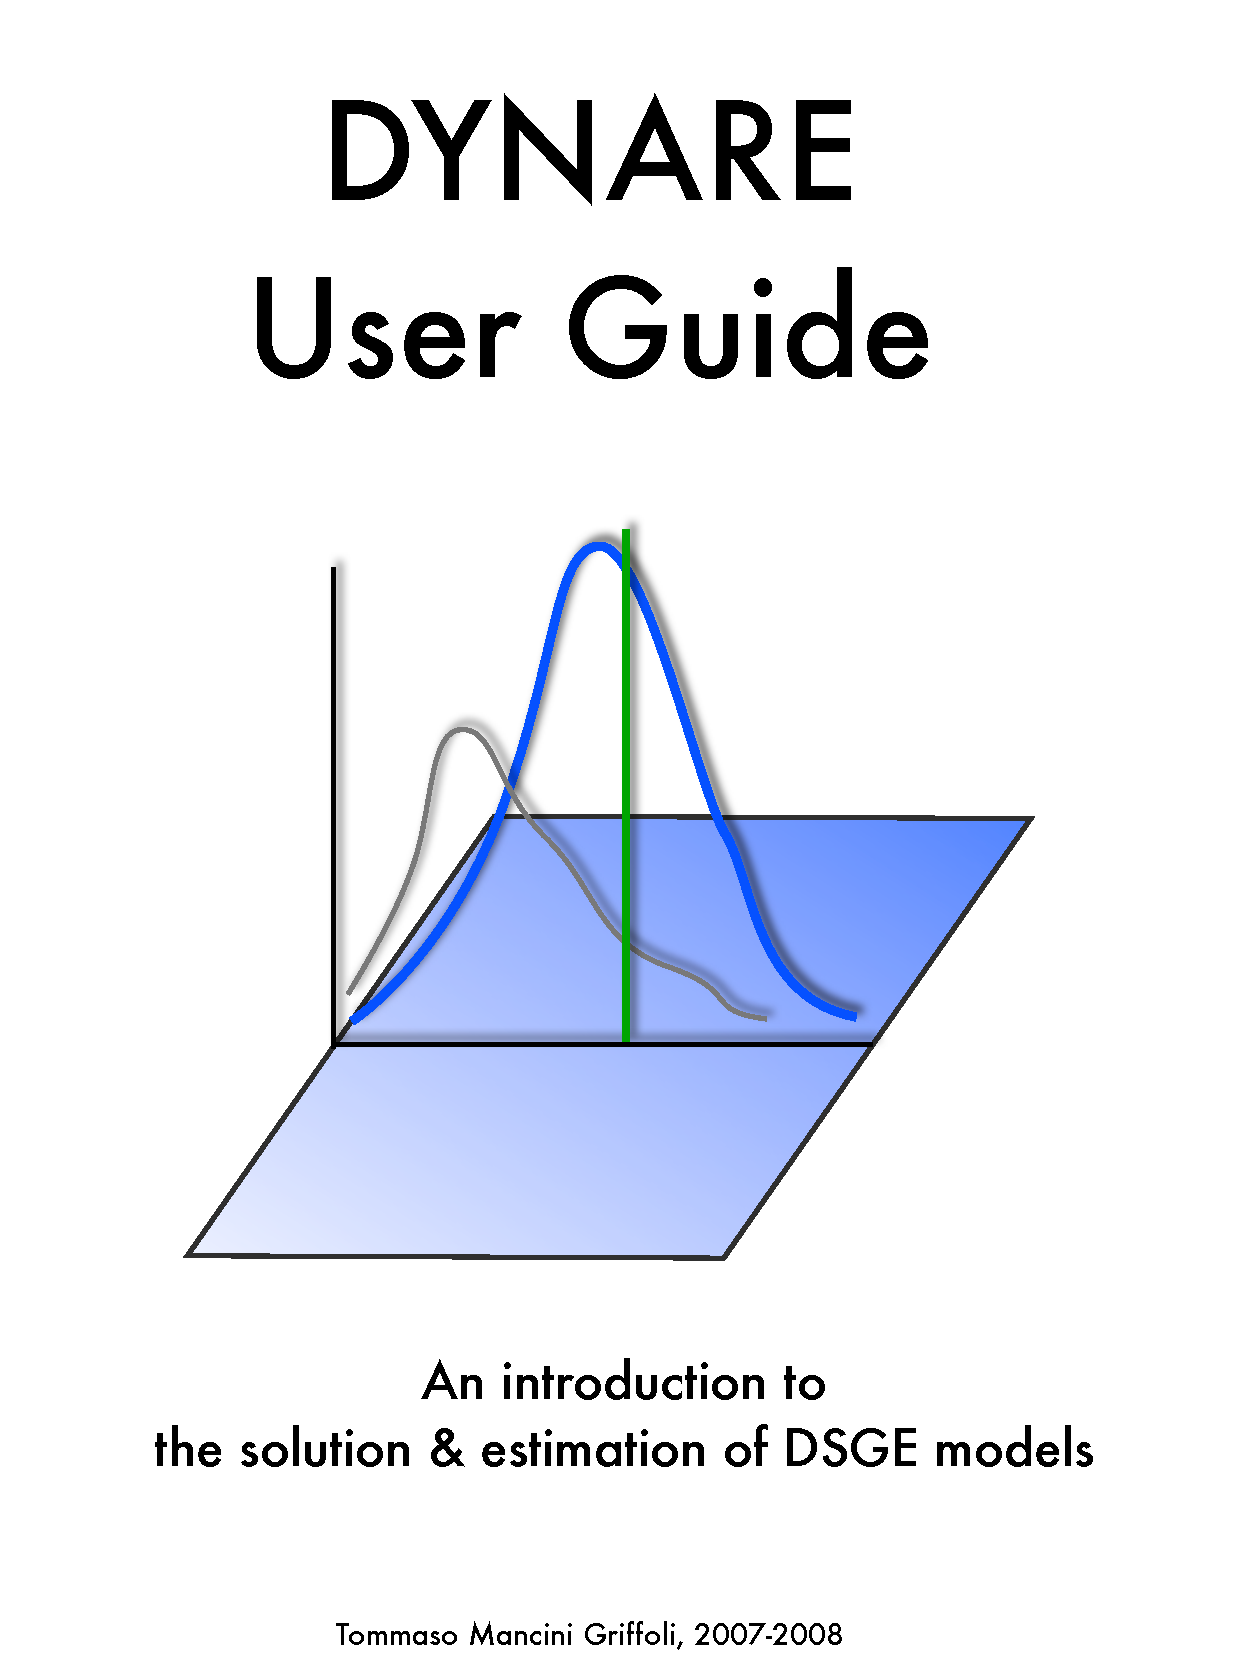
\includepdf{Graphics/DynareTitle.pdf}

\title{Dynare v4 - User Guide \\�Public beta version}
\author{\\ \\ \\ \\ \\ \\ \\ \\ \\ \\ \\  Tommaso Mancini Griffoli\\ tommaso.mancini@stanfordalumni.org}
\date{This draft: November 2009}

\maketitle

\thispagestyle{empty}

\newpage

~\vfill

Copyright � 2007-2009 Tommaso Mancini Griffoli

\bigskip

Permission is granted to copy, distribute and/or modify this document under the terms of the GNU Free Documentation License, Version 1.3 or any later version published by the Free Software Foundation; with no Invariant Sections, no Front-Cover Texts, and no Back-Cover Texts.

\bigskip

A copy of the license can be found at: \url{http://www.gnu.org/licenses/fdl.txt}

\vfill

\newpage

\tableofcontents
\listoffigures

\chapter*{Work in Progress!}
This is the second version of the Dynare User Guide which is still work in progress! This means two things. First, please read this with a critical eye and send me comments! Are some areas unclear? Is anything plain wrong? Are some sections too wordy, are there enough examples, are these clear? On the contrary, are there certain parts that just click particularly well? How can others be improved? I'm very interested to get your feedback. \\

The second thing that a work in progress manuscript comes with is a few internal notes. These are mostly placeholders for future work, notes to myself or others of the Dynare development team, or at times notes to you - our readers - to highlight a feature not yet fully stable. Any such notes are marked with two stars (**). \\

Thanks very much for your patience and good ideas. Please write either direclty to myself: tommaso.mancini@stanfordalumni.org, or \textbf{preferably on the Dynare Documentation Forum} available in the Forum section of the \href{http://www.dynare.org}{Dynare website}. 

\chapter*{Contacts and Credits} \label{ch:contacts}
Dynare was originally developed by Michel Juillard in Paris, France. Currently, the development team of Dynare is composed of

\begin{itemize}
\item St�phane Adjemian (stephane.adjemian``AT''ens.fr)
\item Houtan Bastani
\item Michel Juillard (michel.juillard``AT''ens.fr)
\item Ferhat Mihoubi (ferhat.mihoubi``AT''univ-evry.fr)
\item George Perendia
\item Marco Ratto (marco.ratto``AT''jrc.it)
\item S�bastien Villemot (sebastien.villemot``AT''ens.fr)
\end{itemize}

Several parts of Dynare use or have strongly benefited from publicly available programs by G. Anderson, F. Collard, L. Ingber, O. Kamenik, P. Klein, S. Sakata, F. Schorfheide, C. Sims, P. Soederlind and R. Wouters.

Finally, the development of Dynare could not have come such a long ways withough an active community of users who continually pose questions, report bugs and suggest new features. The help of this community is gratefully acknowledged.\\

The email addresses above are provided in case you wish to contact any one of the authors of Dynare directly. We nonetheless encourage you to first use the \href{http://www.dynare.org/phpBB3}{Dynare forums} to ask your questions so that other users can benefit from them as well; remember, almost no question is specific enough to interest just one person, and yours is not the exception! 

\mainmatter

\chapter{Introduction} \label{ch:intro}

Welcome to Dynare! \\

\section{About this Guide - approach and structure}
This User Guide \textbf{aims to help you master Dynare}'s main functionalities, from getting started to implementing advanced features. To do so, this Guide is structured around examples and offers practical advice. To root this understanding more deeply, though, this Guide also gives some background on Dynare's algorithms, methodologies and underlying theory. Thus, a secondary function of this Guide is to \textbf{serve as a basic primer} on DSGE model solving and Bayesian estimation. \\

This Guide will focus on the most common or useful features of the program, thus emphasizing \textbf{depth over breadth}. The idea is to get you to use 90\% of the program well and then tell you where else to look if you're interested in fine tuning or advanced customization.\\

This Guide is written mainly for an \textbf{advanced economist} - like a professor, graduate student or central banker - needing a powerful and flexible program to support and facilitate his or her research activities in a variety of fields. The sophisticated computer programmer, on the one hand, or the specialist of computational economics, on the other, may not find this Guide sufficiently detailed. \\

We recognize that the ``advanced economist'' may be either a beginning or intermediate user of Dynare. This Guide is written to accommodate both. If you're \textbf{new to Dynare}, we recommend starting with chapters \ref{ch:solbase} and \ref{ch:estbase}, which introduce the program's basic features to solve (including running impulse response functions) and estimate DSGE models, respectively. To do so, these chapters lead you through a complete hands-on example, which we recommend following from A to Z, in order to ``\textbf{learn by doing}''. Once you have read these two chapters, you will know the crux of Dynare's functionality and (hopefully!) feel comfortable using Dynare for your own work. At that point, though, you will probably find yourself coming back to the User Guide to skim over some of the content in the advanced chapters to iron out details and potential complications you may run into.\\

If you're instead an \textbf{intermediate user} of Dynare, you will most likely find the advanced chapters, \ref{ch:soladv} and \ref{ch:estadv}, more appropriate. These chapters cover more advanced features of Dynare and more complicated usage scenarios. The presumption is that you would skip around these chapters to focus on the topics most applicable to your needs and curiosity. Examples are therefore more concise and specific to each feature; these chapters read a bit more like a reference manual.\\

We also recognize that you probably have had repeated if not active exposure to programming and are likely to have a strong economic background. Thus, a black box solution to your needs is inadequate. To hopefully address this issue, the User Guide goes into some depth in covering the \textbf{theoretical underpinnings and methodologies that Dynare follows} to solve and estimate DSGE models. These are available in the ``behind the scenes of Dynare'' chapters \ref{ch:solbeh} and \ref{ch:estbeh}. These chapters can also serve as a \textbf{basic primer} if you are new to the practice of DSGE model solving and Bayesian estimation. \\

Finally, besides breaking up content into short chapters, we've introduced two different \textbf{markers} throughout the Guide to help streamline your reading.
\begin{itemize}
\item \textbf{\textsf{TIP!}} introduces advice to help you work more efficiently with Dynare or solve common problems.  
\item \textbf{\textsf{NOTE!}} is used to draw your attention to particularly important information you should keep in mind when using Dynare. 
\end{itemize} 


\section{What is Dynare?}
Before we dive into the thick of the ``trees'', let's have a look at the ``forest'' from the top \ldots just what is Dynare? \\

\textbf{Dynare is a powerful and highly customizable engine, with an intuitive front-end interface, to solve, simulate and estimate DSGE models}. \\

In slightly less flowery words, it is a pre-processor and a collection of Matlab routines that has the great advantages of reading DSGE model equations written almost as in an academic paper. This not only facilitates the inputting of a model, but also enables you to easily share your code as it is straightforward to read by anyone.\\
\begin{figure} \label{fig:dyn}
\begin{center} 
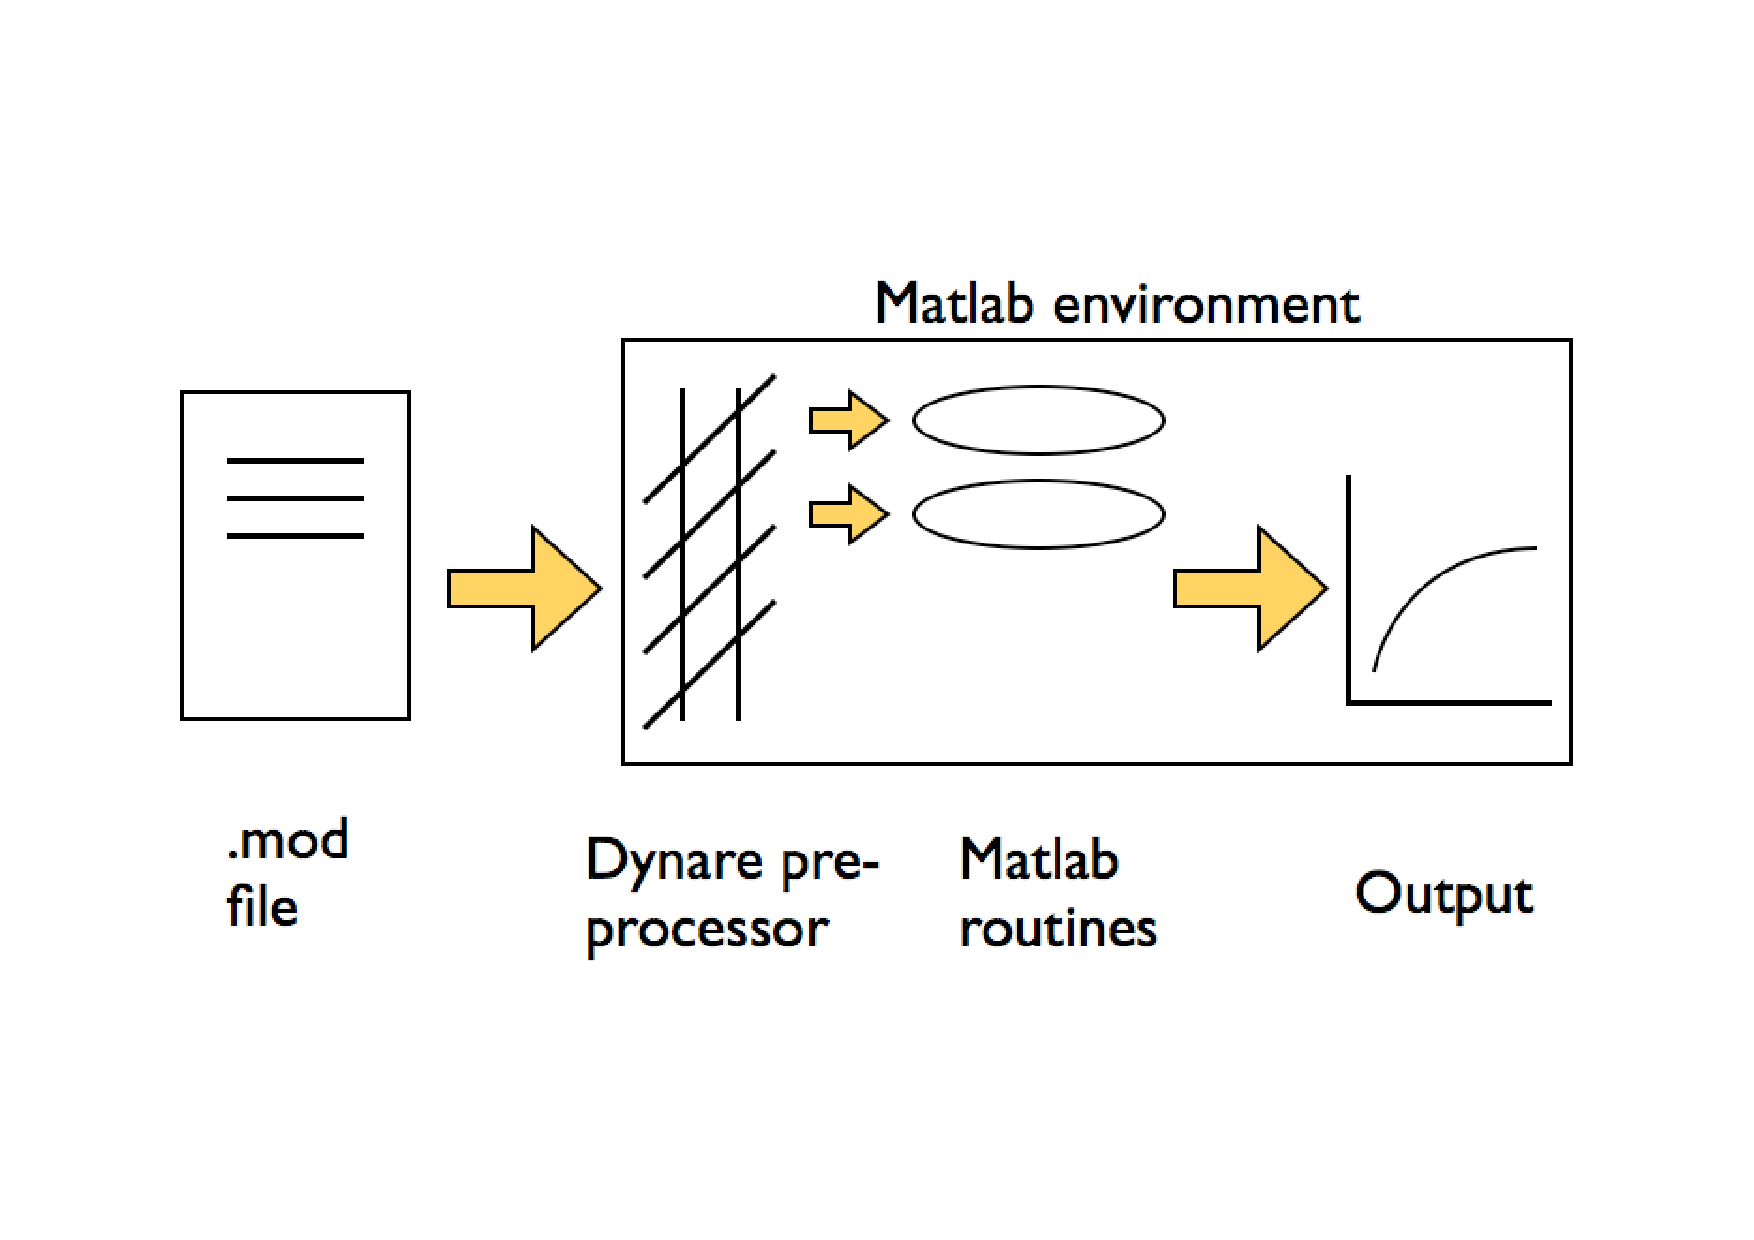
\includegraphics[width=1.0\textwidth]{P_DynareStruct2} 
\end{center} 
\caption[Dynare, a bird's eyeview]{The .mod file being read by the Dynare pre-processor, which then calls the relevant Matlab routines to carry out the desired operations and display the results.} 
\end{figure}

Figure \ref{fig:dyn} gives you an overview of the way Dynare works. Basically, the model and its related attributes, like a shock structure for instance, is written equation by equation in an editor of your choice. The resulting file will be called the .mod file. That file is then called from Matlab. This initiates the Dynare pre-processor which translates the .mod file into a suitable input for the Matlab routines (more precisely, it creates intermediary Matlab or C files which are then used by Matlab code) used to either solve or estimate the model. Finally, results are presented in Matlab. Some more details on the internal files generated by Dynare is given in section \ref{sec:dynfiles} in chapter \ref{ch:soladv}. \\

Each of these steps will become clear as you read through the User Guide, but for now it may be helpful to summarize \textbf{what Dynare is able to do}:
\begin{itemize}
\item compute the steady state of a model
\item compute the solution of deterministic models
\item compute the first and second order approximation to solutions of stochastic models
\item estimate parameters of DSGE models using either a maximum likelihood or a Bayesian approach
\item compute optimal policies in linear-quadratic models
\end{itemize}


\section{Additional sources of help}
While this User Guide tries to be as complete and thorough as possible, you will certainly want to browse other material for help, as you learn about new features, struggle with adapting examples to your own work, and yearn to ask that one question whose answer seems to exist no-where. At your disposal, you have the following additional sources of help:
\begin{itemize}
\item \href{http://www.dynare.org/documentation-and-support/manual}{\textbf{Reference Manual}}: this manual covers all Dynare commands, giving a clear definition and explanation of usage for each. The User Guide will often introduce you to a command in a rather loose manner (mainly through examples); so reading corresponding command descriptions in the Reference Manual is a good idea to cover all relevant details. 
\item \href{http://www.dynare.org/documentation-and-support/examples}{\textbf{Official online examples}}: the Dynare website includes other examples - usually well documented - of .mod files covering models and methodologies introduced in recent papers. 
\item \href{http://www.dynare.org/phpBB3}{\textbf{Dynare forums}}: this lively online discussion forum allows you to ask your questions openly and read threads from others who might have run into similar difficulties. 
\item \href{http://www.dynare.org/documentation-and-support/faq}{\textbf{Frequently Asked Questions}} (FAQ): this section of the Dynare site emphasizes a few of the most popular questions in the forums. 
\item \href{http://www.dsge.net}{\textbf{DSGE.net}}: this website, run my members of the Dynare team, is a resource for all scholars working in the field of DSGE modeling. Besides allowing you to stay up to date with the most recent papers and possibly make new contacts, it conveniently lists conferences, workshops and seminars that may be of interest. 
\end{itemize}

\section{Nomenclature}
To end this introduction and avoid confusion in what follows, it is worthwhile to agree on a few \textbf{definitions of terms}. Many of these are shared with the Reference Manual. 
\begin{itemize}
\item \textbf{Integer} indicates an integer number.
\item \textbf{Double} indicates a double precision number. The following syntaxes are valid: 1.1e3, 1.1E3, 1.1E-3, 1.1d3, 1.1D3
\item \textbf{Expression} indicates a mathematical expression valid in the underlying language (e.g. Matlab).
\item \textbf{Variable name} indicates a variable name. \textbf{\textsf{NOTE!}} These must start with an alphabetical character and can only contain other alphabetical characters and digits, as well as underscores (\_). All other characters, including accents, and \textbf{spaces}, are forbidden. 
\item \textbf{Parameter name} indicates a parameter name which must follow the same naming conventions as above. 
\item \textbf{Filename} indicates a file name valid in your operating system. Note that Matlab requires that names of files or functions start with alphabetical characters; this concerns your Dynare .mod files.
\item \textbf{Command} is an instruction to Dynare or other program when specified. 
\item \textbf{Options} or optional arguments for a command are listed in square brackets \mbox{[ ]} unless otherwise noted. If, for instance, the option must be specified in parenthesis in Dynare, it will show up in the Guide as [(option)].
\item \textbf{\texttt{Typewritten text}} indicates text as it should appear in Dynare code.
\end{itemize}

\section{v4, what's new and backward compatibility}
The current version of Dynare - for which this guide is written - is version 4. With respect to version 3, this new version introduces several important features, as well as improvements, optimizations of routines and bug fixes. The major new features are the following: 
\begin{itemize}
\item Analytical derivatives are now used everywhere (for instance, in the Newton algorithm for deterministic models and in the linearizations necessary to solve stochastic models). This increases computational speed significantly. The drawback is that Dynare can now handle only a limited set of functions, although in nearly all economic applications this should not be a constraint. 
\item Variables and parameters are now kept in the order in which they are declared whenever displayed and when used internally by Dynare. Recall that in version 3, variables and parameters where at times in their order of declaration and at times in alphabetical order. \textbf{\textsf{NOTE!}} This may cause some problems of backward compatibility if you wrote programs to run off Dynare v3 output.
\item The names of many internal variables and the organization of output variables has changed. These are enumerated in details in the relevant chapters. The names of the files internally generated by Dynare have also changed. (** more on this when explaining internal file structure - TBD)
\item The syntax for the external steady state file has changed. This is covered in more details in chapter \ref{ch:solbase}, in section \ref{sec:findsteady}. \textbf{\textsf{NOTE!}} You will unfortunately have to slightly amend any old steady state files you may have written. 
\item Speed. Several large-scale improvements have been implemented to speed up Dynare. This should be most noticeable when solving deterministic models, but also apparent in other functionality.
\end{itemize}


 


\chapter{Installing Dynare} \label{ch:inst}

\section{Dynare versions}
Three versions of Dynare exist: one for \textbf{Matlab}, one for \textbf{Scilab} and one for \textbf{Gauss}. The first benefits from ongoing development and is the most popular. Development of the Scilab version stopped after Dynare version 3.02 and that for Gauss after Dynare version 1.2. \\

This User Guide will exclusively \textbf{focus on the Matlab version of Dynare}. For the installation procedure for the Scilab or Gauss versions of the program, please see the \href{http://www.cepremap.cnrs.fr/juillard/mambo/index.php?option=com_content&task=view&id=51&Itemid=84}{Reference Manual}. Note, though, that the Dynare syntax remains mostly unchanged across the Matlab, Scilab or Gauss versions, for those features common to the three versions. \\

You may also be interested by another version of Dynare, developed in parallel: \textbf{Dynare++}. This is a standalone C++ version of Dynare specialized in computing k-order approximations of dynamic stochastic general equilibrium models. See the \href{http://www.cepremap.cnrs.fr/juillard/mambo/index.php?option=com_content&task=view&id=53&Itemid=86}{Dynare++ webpage} for more information. 

\section{System requirements}
Dynare can run on Windows, as well as Unix-like operating systems, such as any Linux distribution, Solaris and, of course, Mac OS X. If you have questions about the support of a particular platform, feel free to write directly to Michel Juillard (michel.juillard"AT"ens.fr) or visit the \href{http://www.cepremap.cnrs.fr/juillard/mambo/index.php?option=com_forum&Itemid=95&page=viewforum&f=1}{\textbf{Dynare forums}}. \\

To run Dynare, it is recommended to allocate at least 256MB of RAM to the platform running Dynare, although 512MB is preferred. Depending on the type of computations required, like the very processor intensive Metropolis Hastings algorithm, you may need up to 1GB of RAM to obtain acceptable computational times. \\

\section{Installing Dynare}
\subsection{Installing on Windows}
The following assumes you have Matlab version 6.5.1 or later installed on your Windows system.\footnote{As of writing this Guide, Dynare is being developed on Matlab version 7. Nonetheless, great care is taken not to introduce features that would not work with reasonably recent versions of Matlab. However, Dynare requires at least the Matlab feature set of version 6.5.1, released September 22, 2003.} ** The current way to install Dynare version 4 may not yet be on par with the procedure described below. If a discrepancy exists, please follow downloading and installation instructions on the Dynare website. \begin{enumerate}
\item Download the latest stable version of Dynare for Matlab (Windows) from the \href{http://www.cepremap.cnrs.fr/juillard/mambo/index.php?option=com_frontpage&Itemid=1}{Dynare website}. 
\item You will now have on your computer a .zip file which you should unzip. This will create a folder called, by default, Dynare and its version number, for example: Dynare\_v4.x (where $x$ stands for any subsequent upgrades). 
\item This directory contains several sub-directories, among which (i) matlab, (ii) doc and (iii) examples. 
\item Place the Dynare folder (Dynare\_v4.x in our example) in the c: directory and note that location. The easiest is probably to put it in the root of c: as in c:/dynare\_v4.x.
\item Start Matlab and use the menu File/Set-Path to add the path to the Dynare 
matlab subdirectory. Following our example, this would correspond to 
c:/dynare\_v4.x/matlab
\item Save these changes in Matlab and you're ready to go.
\end{enumerate} 


\section{Matlab particularities}

A question often comes up: what special Matlab toolboxes are necessary to run Dynare? In fact, no additional toolbox is necessary for running most of Dynare, except maybe for optimal simple rules (see chapter \ref{ch:ramsey}), but even then remedies exist (see the \href{http://www.cepremap.cnrs.fr/juillard/mambo/index.php?option=com_forum&Itemid=95}{Dynare forums} for discussions on this, or to ask your particular question). But if you do have the `optimization toolbox' installed, you will have additional options for solving for the steady state (solve\_algo option) and for searching for the posterior mode (mode\_compute option), both of which are defined later. 



\chapter{Solving DSGE models - basics} \label{ch:solbase}

This chapter covers everything that leads to, and stems from, the solution of DSGE models; a vast terrain. That is to say that the term ``solution'' in the title of the chapter is used rather broadly. You may be interested in simply finding the solution functions to a set of first order conditions stemming from your model, but you may also want to go a bit further. Typically, you may be interested in how this system behaves in response to shocks, whether temporary or permanent. Likewise, you may want to explore how the system comes back to its steady state or moves to a new one. This chapter covers all these topics. But instead of skipping to the topic closest to your needs, we recommend that you read this chapter chronologically, to learn basic Dynare commands and the process of writing a proper .mod file - this will serve as a base to carry out any of the above computations. 

\section{A fundamental distinction} \label{sec:distcn}
Before speaking of Dynare, it is important to recognize a distinction in model types. This distinction will appear throughout the chapter; in fact, it is so fundamental, that we considered writing separate chapters altogether. But the amount of common material - Dynare commands and syntax - is notable and writing two chapters would have been overly repetitive. Enough suspense; here is the important question: \textbf{is your model stochastic or deterministic?}\\

The distinction hinges on \textbf{whether future shocks are known}. In deterministic models, the occurrence of all future shocks is known exactly at the time of computing the model's solution. In stochastic models, instead, only the distribution of future shocks is known. Let's consider a shock to a model's innovation only in period 1. In a deterministic context, agents will take their decisions knowing that future values of the innovations will be zero in all periods to come. In a stochastic context, agents will take their decisions knowing that the future value of innovations are random but will have zero mean. This isn't the same thing because of Jensen's inequality. Of course, if you consider only a first order linear approximation of the stochastic model, or a linear model, the two cases become practically the same, due to certainty equivalence. A second order approximation will instead lead to very different results, as the variance of shocks will matter. \\

The solution method for each of these model types differs significantly. In deterministic models, a highly accurate solution can be found by numerical methods. The solution is nothing more than a series of numbers that match a given set of equations. Intuitively, if an agent has perfect foresight, she can specify today - at the time of making her decision - what each of her precise actions will be in the future. In a stochastic environment, instead, the best the agent can do is specify a decision, policy or feedback rule for the future: what will her optimal actions be contingent on each possible realization of shocks. In this case, we therefore search for a function satisfying the model's first order conditions. To complicate things, this function may be non-linear and thus needs to be approximated. In control theory, solutions to deterministic models are usually called ``closed loop'' solutions, and those to stochastic models are referred to as ``open loop''.\\

Because this distinction will resurface again and again throughout the chapter, but also because it has been a source of significant confusion in the past, the following gives some additional details. 

\subsection{\textsf{NOTE!} Deterministic vs stochastic models} \label{sec:detstoch}

\textbf{Deterministic} models have the following characteristics:
\begin{enumerate}
\item As the DSGE (read, ``stochastic'', i.e. not deterministic!) literature has gained attention in economics, deterministic models have become somewhat rare. Examples include OLG models without aggregate uncertainty.
\item These models are usually introduced to study the impact of a change in regime, as in the introduction of a new tax, for instance. 
\item Models assume full information, perfect foresight and no uncertainty around shocks.
\item Shocks can hit the economy today or at any time in the future, in which case they would be expected with perfect foresight. They can also last one or several periods.
\item Most often, though, models introduce a positive shock today and zero shocks thereafter (with certainty).
\item The solution does not require linearization, in fact, it doesn't even really need a steady state. Instead, it involves numerical simulation to find the exact paths of endogenous variables that meet the model's first order conditions and shock structure. 
\item This solution method can therefore be useful when the economy is far away from steady state (when linearization offers a poor approximation).
\end{enumerate}
\textbf{Stochastic} models, instead, have the following characteristics:
\begin{enumerate}
\item These types of models tend to be more popular in the literature. Examples include most RBC models, or new keynesian monetary models.
\item In these models, shocks hit today (with a surprise), but thereafter their expected value is zero. Expected future shocks, or permanent changes in the exogenous variables cannot be handled due to the use of Taylor approximations around a steady state.
\item Note that when these models are linearized to the first order, agents behave as if future shocks where equal to zero (since their expectation is null), which is the \textbf{certainty equivalence property}. This is an often overlooked point in the literature which misleads readers in supposing their models may be deterministic.
\end{enumerate}


\section{Introducing an example}
The goal of this first section is to introduce a simple example. Future sections will aim to code this example into Dynare and analyze its salient features under the influence of shocks - both in a stochastic and a deterministic environment. Note that as a general rule, the examples in the basic chapters, \ref{ch:solbase} and \ref{ch:estbase}, are kept as bare as possible, with just enough features to help illustrate Dynare commands and functionalities. More complex examples are instead presented in the advanced chapters.\\

The model introduced here is a basic RBC model with monopolistic competition, used widely in the literature. Its particular notation adopted below is drawn mostly from notes available on Jesus Fernandez-Villaverde's very instructive \href{http://www.econ.upenn.edu/~jesusfv/}{website}; this is a good place to look for additional information on any of the following model set-up and discussion. Note throughout this model description that the use of \textbf{expectation} signs is really only relevant in a stochastic setting, as per the earlier discussion. We will none-the-less illustrate both the stochastic and the deterministic settings on the basis of this example. Thus, when thinking of the latter, you'll have to use a bit of imagination (on top of that needed to think you have perfect foresight!) to ignore the expectation signs.\\

Households maximize utility over consumption, $c_t$ and leisure, $1-l_t$, where $l_t$ is labor input, according to the following utility function
\[
\mathbb{E}_t \sum_{t=0}^{\infty} \beta \left[ \log c_t + \psi \log(1-l_t) \right]
\]
and subject to the following budget constraint
\[
c_t + k_{t+1}=w_t l_t + r_t k_t + (1-\delta)k_t, \qquad \forall t>0
\]
where $k_t$ is capital stock, $w_t$ real wages, $r_t$ real interest rates or cost of capital and $\delta$ the depreciation rate. \\

The above equation can be seen as an accounting identity, with total expenditures on the left hand side and revenues - including the liquidation value of the capital stock - on the right hand side. Alternatively, with a little more imagination, the equation can also be interpreted as a capital accumulation equation after bringing $c_t$ to the right hand side and noticing that $w_t l_t + r_t k_t$, total payments to factors, equals $y_t$, or aggregate output, by the zero profit condition. As a consequence, if we define investment as $i_t=y_t - c_t$, we obtain the intuitive result that $i_t=k_{t+1} - (1-\delta) k_{t}$, or that investment replenishes the capital stock thereby countering the effects of depreciation. In any given period, the consumer therefore faces a tradeoff between consuming and investing in order to increase the capital stock and consuming more in following periods (as we will see later, production depends on capital).\\

Maximization of the household problem with respect to consumption, leisure and capital stock, yields the Euler equation in consumption, capturing the intertemporal tradeoff mentioned above, and the labor supply equation linking labor positively to wages and negatively to consumption (the wealthier, the more leisure due to the decreasing marginal utility of consumption). These equation are
\[
\frac{1}{c_t}=\beta \mathbb{E}_t \left[ \frac{1}{c_{t+1}} \left( 1 + r_{t+1} - \delta \right) \right]
\]
and
\[
\psi \frac{c_t}{1-l_t}= w_t
\]

The firm side of the problem is slightly more involved, due to monopolistic competition, but is presented below in the simplest possible terms, with a little hand-waiving involved, as the derivations are relatively standard. \\

There are two ways to introduce monopolistic competition. We can either assume that firms sell differentiated varieties of a good to consumers who aggregate these according to a CES index. Or we can postulate that there is a continuum of intermediate producers with market power who each sell a different variety to a competitive final goods producer whose production function is a CES aggregate of intermediate varieties.\\

If we follow the second route, the final goods producer chooses his or her optimal demand for each variety, yielding the Dixit-Stiglitz downward sloping demand curve. Intermediate producers, instead, face a two pronged decision: how much labor and capital to employ given these factors' perfectly competitive prices and how to price the variety they produce.\\

Production of intermediate goods follows a CRS production function defined as
\[
y_{it} = k_{it}^\alpha (e^{z_t} l_{it})^{1-\alpha}
\]
where the $i$ subscript stands for firm $i$ of a continuum of firms between zero and one and where $\alpha$ is the capital elasticity in the production function, with $0<\alpha<1$. Also, $z_t$ captures technology which evolves according to
\[
z_t = \rho z_{t-1} + e_t
\]
where $\rho$ is a parameter capturing the persistence of technological progress and $e_t \thicksim \mathcal{N}(0,\sigma)$. \\

The solution to the sourcing problem yields an optimal capital to labor ratio, or relationship between payments to factors:
\[
k_{it}r_t=\frac{\alpha}{1-\alpha}w_tl_{it}
\]

The solution to the pricing problem, instead, yields the well-known constant markup pricing condition of monopolistic competition:
\[
p_{it}=\frac{\epsilon}{\epsilon -1}mc_t p_t
\]
where $p_{it}$ is firm $i$'s specific price, $mc_t$ is real marginal cost and $p_t$ is the aggregate CES price or average price. An additional step simplifies this expression: symmetric firms implies that all firms charge the same price and thus $p_{it}=p_t$; we therefore have: $mc_t = (\epsilon - 1)/\epsilon$ \\

But what are marginal costs equal to? To find the answer, we combine the optimal capital to labor ratio into the production function and take advantage of its CRS property to solve for the amount of labor or capital required to produce one unit of output. The real cost of using this amount of any one factor is given by $w_tl_{it} + r_tk_{it}$ where we substitute out the payments to the other factor using again the optimal capital to labor ratio. When solving for labor, for instance, we obtain
\[
mc_t = \left( \frac{1}{1-\alpha}�\right)^{1-\alpha} \left( \frac{1}{\alpha}�\right)^\alpha \frac{1}{A_t}w_t^{1-\alpha} r_t^\alpha
\]
which does not depend on $i$; it is thus the same for all firms. \\

Interestingly, the above can be worked out, by using the optimal capital to labor ratio, to yield $w_t [(1-\alpha)y_{it}/l_{it}]^{-1}$, or $w_t \frac{\partial l_{it}}{\partial y_{it}}$, which is the definition of marginal cost: the cost in terms of labor input of producing an additional unit of output. This should not be a surprise since the optimal capital to labor ratio follows from the maximization of the production function (minus real costs) with respect to its factors. \\

Combining this result for marginal cost, as well as its counterpart in terms of capital, with the optimal pricing condition yields the final two important equations of our model
\[
w_t = (1-\alpha) \frac{y_{it}}{l_{it}} \frac{(\epsilon-1)}{\epsilon}
\]
and
\[
r_t = \alpha \frac{y_{it}}{k_{it}} \frac{(\epsilon-1)}{\epsilon}
\]

To end, we aggregate the production of each individual firm to find an aggregate production function. On the supply side, we factor out the capital to labor ratio, $k_t/l_t$, which is the same for all firms and thus does not depend on $i$. On the other side, we have the Dixit-Stiglitz demand for each variety. By equating the two and integrating both side, and noting that price dispersion is null - or that, as hinted earlier, $p_{it}=p_t$ - we obtain aggregate production
\[
y_t = A_t k_t^\alpha l_t^{1-\alpha}
\]
which can be shown is equal to the aggregate amount of varieties bought by the final good producer (according to a CES aggregation index) and, in turn, equal to the aggregate output of final good, itself equal to household consumption. Note, to close, that because the ratio of output to each factor is the same for each intermediate firm and that firm specific as well as aggregate production is CRS, we can rewrite the above two equations for $w_t$ and $r_t$ without the $i$ subscripts on the right hand side. \\

This ends the exposition of the example. Now, let's roll up our sleeves and see how we can input the model into Dynare and actually test how the model will respond to shocks. 

\section{Dynare .mod file structure}
Input into Dynare involves the .mod file, as mentioned loosely in the introduction of this Guide. The .mod file can be written in any editor, external or internal to Matlab. It will then be read by Matlab by first navigating within Matlab to the directory where the .mod file is stored and then by typing in the Matlab command line \texttt{Dynare filename.mod;} (although actually typing the extension .mod is not necessary). But before we get into executing a .mod file, let's start by writing one! \\

It is convenient to think of the .mod file as containing four distinct blocks, illustrated in figure \ref{fig:modstruct}:
\begin{itemize}
\item \textbf{preamble}: lists variables and parameters
\item \textbf{model}: spells out the model
\item \textbf{steady state or initial value}: gives indications to find the steady state of a model, or the starting point for simulations or impulse response functions based on the model's solution. 
\item \textbf{shocks}: defines the shocks to the system
\item \textbf{computation}: instructs Dynare to undertake specific operations (e.g. forecasting, estimating impulse response functions)
\end{itemize}
Our exposition below will structured according to each of these blocks. 
\begin{figure} \label{fig:modstruct}
\begin{center} 
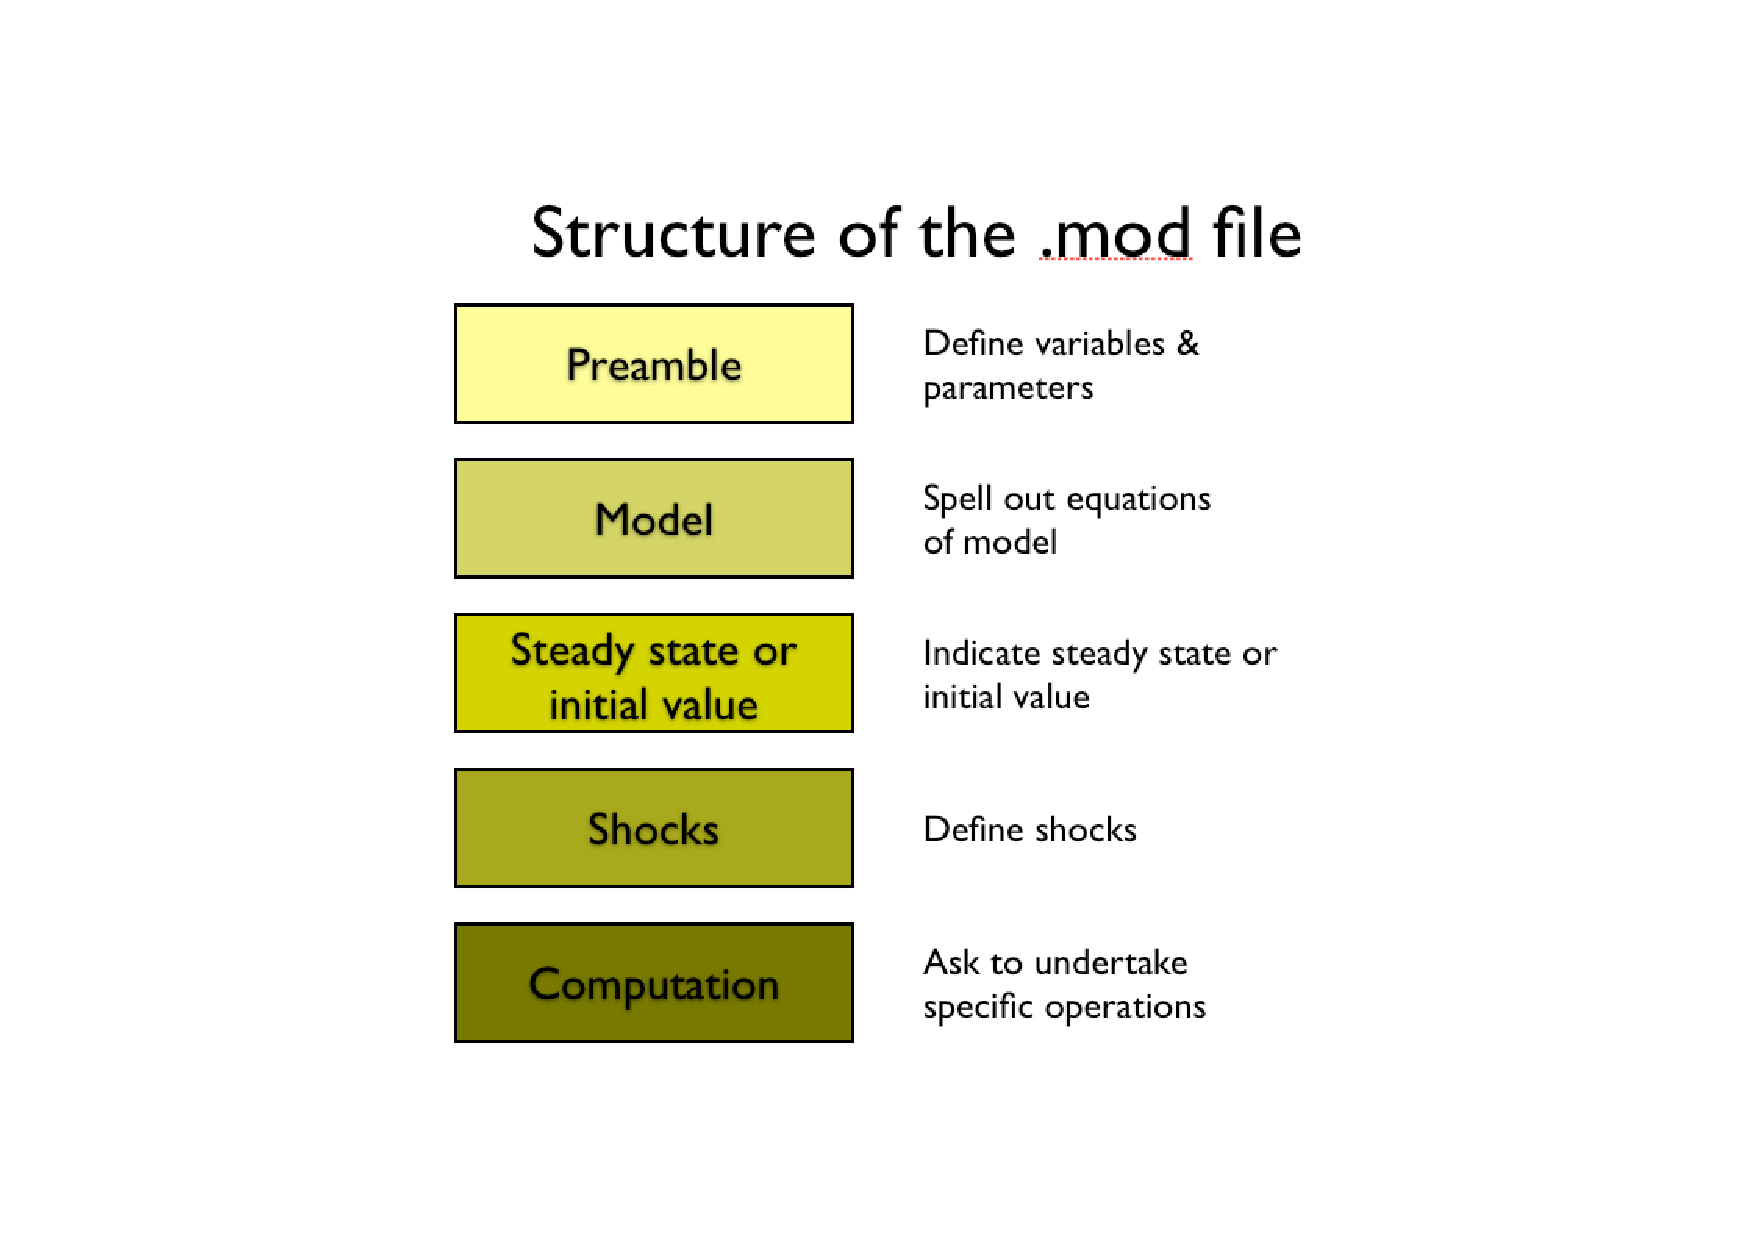
\includegraphics[width=1.0\textwidth]{P_ModStruct5} 
\end{center} 
\caption[Structure of the .mod file]{The .mod file contains five logically distinct parts.} 
\end{figure}

\section{Filling out the preamble} \label{sec:preamble}
The preamble generally involves three commands that tell Dynare what are the model's variables, which are endogenous and what are the parameters. The \textbf{commands} are:
\begin{itemize}
\item \texttt{var} starts the list of endogenous variables, to be separated by commas. 
\item \texttt{varexo} starts the list of exogenous variables that will be shocked.
\item \texttt{parameters} starts the list of parameters and assigns values to each.
\end{itemize}
In the case of our example, let's differentiate between the stochastic and deterministic cases. First, we lay these out, then we discuss them. 

\subsection{The deterministic case}
The model is inherited exactly as specified in the earlier description, except that we no longer need the $e_t$ variable, as we can make $z_t$ directly exogenous. Thus, the \textbf{preamble would look like}:\\
\\
\texttt{var y c k i l y\_l w r;\\
varexo z;\\
parameters beta psi delta alpha sigma epsilon;\\
alpha   = 0.33;\\
beta    = 0.99;\\
delta   = 0.023;\\
psi     = 1.75;\\
sigma   = (0.007/(1-alpha));\\
epsilon = 10;}\\

\subsection{The stochastic case}
In this case, we go back to considering the law of motion for technology, consisting of an exogenous shock, $e_t$. With respect to the above, we therefore adjust the list of endogenous and exogenous variables, and add the parameter $\rho$. Here's what the \textbf{preamble would look like}:\\ 
\\
\texttt{var y c k i l y\_l w r  z;\\
varexo e;\\
parameters beta psi delta alpha rho sigma epsilon;\\
alpha   = 0.33;\\
beta    = 0.99;\\
delta   = 0.023;\\
psi     = 1.75;\\
rho     = 0.95; \\ 
sigma   = (0.007/(1-alpha));\\
epsilon = 10;}\\

\subsection{Comments on your first lines of Dynare code}

As you can tell, writing a .mod file is really quite straightforward. Two quick comments:\\

\textsf{\textbf{NOTE!}} Remember that each instruction of the .mod file must be terminated by a semicolon (;), although a single instruction can span two lines if you need extra space (just don't put a semicolon at the end of the first line).\\

\textsf{\textbf{TIP!}} You can also comment out any line by starting the line with two forward slashes (//), or comment out an entire section by starting the section with /* and ending with */. For example:\\
\\
\texttt{var y c k i l y\_l w r  z;\\
varexo e;\\
parameters beta psi delta \\
alpha rho sigma epsilon;\\
// the above instruction reads over two lines\\
/*\\
the following section lists\\
several parameters which were\\
calibrated by my co-author. Ask\\
her all the difficult questions!\\
*/\\
alpha   = 0.33;\\
beta    = 0.99;\\
delta   = 0.023;\\
psi     = 1.75;\\
rho     = 0.95; \\ 
sigma   = (0.007/(1-alpha));\\
epsilon = 10;}\\  
\\

\section{Specifying the model} \label{sec:modspe}
\subsection{Model in Dynare notation}
One of the beauties of Dynare is that you can \textbf{input your model's equations naturally}, almost as if you were writing them in an academic paper. This greatly facilitates the sharing of your Dynare files, as your colleagues will be able to understand your code in no-time. There are just a few conventions to follow. Let's first have a look at our \textbf{model in Dynare notation}, and then go through the various Dynare input conventions. What you can already try to do is glance at the model block below and see if you can recognize the equations from the earlier example. See how easy it is to read Dynare code? \\
\\
\texttt{model;\\
  (1/c) = beta*(1/c(+1))*(1+r(+1)-delta);\\
  psi*c/(1-l) = w;\\
  c+i = y;\\
  y = (k(-1)\textasciicircum alpha)*(exp(z)*l)\textasciicircum (1-alpha);\\
  w = y*((epsilon-1)/epsilon)*(1-alpha)/l;\\
  r = y*((epsilon-1)/epsilon)*alpha/k(-1);\\
  i = k-(1-delta)*k(-1);\\
  y\_l = y/l;\\
  z = rho*z(-1)+e;\\
end;}\\

Just in case you need a hint or two to recognize these equations, here's a brief description: the first equation is the Euler equation in consumption. The second the labor supply function. The third the accounting identity. The fourth is the production function. The fifth and sixth are the marginal cost equal to markup equations. The seventh is the investment equality. The eighth an identity that may be useful and the last the equation of motion of technology.

\textsf{\textbf{NOTE!}} that the above model specification corresponds to the \textbf{stochastic case}; indeed, notice that the law of motion for technology is included, as per our discussion of the preamble. The corresponding model for the \textbf{deterministic casce} would simply loose the last equation. 

\subsection{General conventions}
The above example illustrates the use of a few important commands and conventions to translate a model into a Dynare-readable .mod file. 
\begin{itemize}
\item The first thing to notice, is that the model block of the .mod file begins with the command \texttt{model} and ends with the command \texttt{end}. 
\item Second, in between, there need to be as many equations as you declared endogenous variables (this is actually one of the first things that Dynare checks; it will immediately let you know if there are any problems). 
\item Third, as in the preamble and everywhere along the .mod file, each line of instruction ends with a semicolon (except when a line is too long and you want to break it across two lines. This is unlike Matlab where if you break a line you need to add \ldots). 
\item Fourth, equations are entered one after the other; no matrix representation is necessary. Note that variable and parameter names used in the model block must be the same as those declared in the preamble; \textsf{\textbf{TIP!}} remember that variable and parameter names are case sensitive. 
\end{itemize}

\subsection{Notational conventions}

\begin{itemize}
\item Variables entering the system with a time $t$ subscript are written plainly. For example, $x_t$ would be written $x$. 
\item Variables entering the system with a time $t-n$ subscript are written with $(-n)$ following them. For example, $x_{t-2}$ would be written $x(-2)$ (incidentally, this would count as two backward looking variables). 
\item In the same way, variables entering the system with a time $t+n$ subscript are written with $(+n)$ following them. For example, $x_{t+2}$ would be written $x(+2)$. Writing $x(2)$ is also allowed, but this notation makes it slightly harder to count by hand the number of forward looking variables (a useful measure to check); more on this below \ldots
\end{itemize}

\subsection{Timing conventions}
\begin{itemize}
\item In Dynare, the timing of each variable reflects when that variable is decided. For instance, our capital stock is not decided today, but yesterday (recall that it is a function of yesterday's investment and capital stock); it is what we call in the jargon a \textbf{predetermined} variable. Thus, eventhough in the example presented above we wrote $k_{t+1}=i_t + (1-\delta)k_t$, as in many papers, we would translate this equation into Dynare as \texttt{k=i+(1-delta)*k(-1)}.
\item As another example, consider that in some wage negociation models, wages used during a period are set the period before. Thus, in the equation for wages, you can write wage in period $t$ (when they are set), but in the labor demand equation, wages should appear with a one period lag.
\item A slightly more roundabout way to explain the same thing is that for stock variables, you must use a ``stock at the end of the period'' concept. It is investment during period $t$ that sets stock at the end of period $t$. Be careful, a lot of papers use the ``stock at the beginning of the period'' convention, as we did (on purpose to highlight this distinction!) in the setup of the example model above. 
\end{itemize}

\subsection{Conventions specifying non-predetermined variables}
\begin{itemize}
\item A (+1) next to a variable tells Dynare to count the occurrence of that variable as a jumper or forward-looking or non-predetermined variable. 
\item \textbf{Blanchard-Kahn} conditions are met only if the number of non-predetermined variables equals the number of eigenvalues greater than one. If this condition is not met, Dynare will put up a warning. 
\item Note that a variable may occur both as predetermined and non-predetermined. For instance, consumption could appear with a lead in the Euler equation, but also with a lag in a habit formation equation, if you had one. In this case, the second order difference equation would have two eigenvalues, one needing to be greater and the other smaller than one for stability. 
\end{itemize}

\subsection{Linear and log-linearized models}
There are two other variants of the system's equations which Dynare accommodates. First, the \textbf{linear model} and second, the \textbf{model in exp-logs}. In the first case, all that is necessary is to write the term \texttt{(linear)} next to the command \texttt{model}. Our example, with just the equation for $y_l$ for illustration, would look like:\\
\\
\texttt{model (linear);\\
yy\_l=yy - ll;\\
end;}\\
\\
where repeating a letter for a variable means difference from steady state.\\

Otherwise, you may be interested to have Dynare take Taylor series expansions in logs rather than in levels; this turns out to be a very useful option when estimating models with unit roots, as we will see in chapter \ref{ch:estbase}. If so, simply rewrite your equations by taking the exponential and logarithm of each variable. The Dynare input convention makes this very easy to do. Our example would need to be re-written as follows (just shown for the first two equations)\\
\\
\texttt{model;\\
  (1/exp(cc)) = beta*(1/exp(cc(+1)))*(1+exp(rr(+1))-delta);\\
  psi*exp(cc)/(1-exp(ll)) = exp(ww);\\
  end;}\\
  \\
  where, this time, repeating a letter for a variable means log of that variable, so that the level of a variable is given by $exp(repeated variable)$.

\section{Specifying steady states and/or initial values} \label{sec:ssshock}
Material in this section has created much confusion in the past. But with some attention to the explanations below, you should get through unscathed. Let's start by emphasizing the uses of this section of the .mod file. First, recall that stochastic models need to be linearized. Thus, they need to have a steady state. One of the functions of this section is indeed to provide these steady state values, or approximations of values. Second, irrespective of whether you're working with a stochastic or deterministic model, you may be interested to start your simulations or impulse response functions from either a steady state, or another given point. This section is also useful to specify this starting value. Let's see in more details how all this works.\\

In passing, though, note that the relevant commands in this section are \texttt{initval}, \texttt{endval} or, more rarely, \texttt{histval} which is covered only in the \href{http://www.dynare.org/documentation-and-support/manual}{Reference Manual}. The first two are instead covered in what follows. \\

\subsection{Stochastic models and steady states}
In a stochastic setting, your model will need to be linearized before it is solved. To do so, Dynare needs to know your model's steady state (more details on finding a steady state, as well as tips to do so more efficiently, are provided in section \ref{sec:findsteady} below). You can either enter exact steady state values into your .mod file, or just approximations and let Dynare find the exact steady state (which it will do using numerical methods based on your approximations). In either case, these values are entered in the \texttt{initval} block, as in the following fashion: \\
\\
\texttt{initval;\\
  k = 9;\\
  c = 0.7;\\
  l = 0.3;\\
  w = 2.0;\\
  r = 0;\\
  z = 0; \\
  e = 0;\\
end;}
\\

Then, by using the command \texttt{steady}, you can control whether you want to start your simulations or impulse response functions from the steady state, or from the exact values you specified in the \texttt{initval} block. Adding \texttt{steady} just after your \texttt{initval} block will instruct Dynare to consider your initial values as mere approximations and start simulations or impulse response functions from the exact steady state. On the contrary, if you don't add the command \texttt{steady}, your simulations or impulse response functions will start from your initial values, even if Dynare will have calculated your model's exact steady state for the purpose of linearization. \\

For the case in which you would like simulations and impulse response functions to begin at the steady state, the above block would be expanded to yield:\\
\\
\texttt{initval;\\
  k = 9;\\
  c = 0.7;\\
  l = 0.3;\\
  w = 2.0;\\
  r = 0;\\
  z = 0; \\
  e = 0;\\
end;\\
\\
steady;}
\\

\textsf{\textbf{TIP!}} If you're dealing with a stochastic model, remember that its linear approximation is good only in the vicinity of the steady state, thus it is strongly recommended that you start your simulations from a steady state; this means either using the command \texttt{steady} or entering exact steady state values. \\


\subsection{Deterministic models and initial values}
Deterministic models do not need to be linearized in order to be solved. Thus, technically, you do not need to provide a steady state for these model. But practically, most researchers are still interested to see how a model reacts to shocks when originally in steady state. In the deterministic case, the \texttt{initval} block serves very similar functions as described above. If you wanted to shock your model starting from a steady state value, you would enter approximate (or exact) steady state values in the \texttt{initval} block, followed by the command \texttt{steady}. Otherwise, if you wanted to begin your solution path from an arbitrary point, you would enter those values in your \texttt{initval} block and not use the \texttt{steady} command. An illustration of the \texttt{initval} block in the deterministic case appears further below. \\

\subsection{Finding a steady state} \label{sec:findsteady}

The difficulty in the above, of course, is calculating actual steady state values. Doing so borders on a form of art, and luck is unfortunately part of the equation. Yet, the following \textsf{\textbf{TIPS!}} may help.\\

As mentioned above, Dynare can help in finding your model's steady state by calling the appropriate Matlab functions. But it is usually only successful if the initial values you entered are close to the true steady state. If you have trouble finding the steady state of your model, you can begin by playing with the \textbf{options following the \texttt{steady} command}. These are:
\begin{itemize}
\item \texttt{solve\_algo = 0}: uses Matlab Optimization Toolbox FSOLVE
\item \texttt{solve\_algo = 1}: uses Dynare�s own nonlinear equation solver
\item \texttt{solve\_algo = 2}: splits the model into recursive blocks and solves each block in turn. 
\item \texttt{solve\_algo = 3}: uses the Sims solver. This is the default option if none are specified.
\end{itemize}

For complicated models, finding suitable initial values for the endogenous variables is the trickiest part of finding the equilibrium of that model. Often, it is better to start with a smaller model and add new variables one by one.\\

But even for simpler models, you may still run into difficulties in finding your steady state. If so, another option is to \textbf{enter your model in linear terms}. In this case, variables would be expressed in percent deviations from steady state. Thus, their initial values would all be zero. Unfortunately, if any of your original (non-linear) equations involve sums (a likely fact), your linearized equations will include ratios of steady state values, which you would still need to calculate. Yet, you may be left needing to calculate fewer steady state values than in the original, non-linear, model. \\

Alternatively, you could also use an \textbf{external program to calculate exact steady state values}. For instance, you could write an external \textbf{Maple} file and then enter the steady state solution by hand in Dynare. But of course, this procedure could be time consuming and bothersome, especially if you want to alter parameter values (and thus steady states) to undertake robustness checks. \\

The alternative is to write a \textbf{Matlab} program to find your model's steady state. Doing so has the clear advantages of being able to incorporate your Matlab program directly into your .mod file so that running loops with different parameter values, for instance, becomes seamless. \textsf{\textbf{NOTE!}} When doing so, your matlab (.m) file should have the same name as your .mod file, followed by \texttt{\_steadystate} For instance, if your .mod file is called \texttt{example.mod}, your Matlab file should be called \texttt{example\_steadystate.m} and should be saved in the same directory as your .mod file. Dynare will automatically check the directory where you've saved your .mod file to see if such a Matlab file exists. If so, it will use that file to find steady state values regardless of whether you've provided initial values in your .mod file. \\

Because Matlab does not work with analytical expressions, though (unless you're working with a particular toolbox), you need to do a little work to write your steady state program. It is not enough to simply input the equations as you've written them in your .mod file and ask Matlab to solve the system. You will instead need to write your steady state program as if you were solving for the steady state by hand. That is, you need to input your expressions sequentially, whereby each left-hand side variable is written in terms of known parameters or variables already solved in the lines above. For example, the steady state file corresponding to the above example, in the stochastic case, would be: (** example file to be added shortly) \\

\subsection{Checking system stability}
\textsf{\textbf{TIP!}} A handy command that you can add after the \texttt{initval} or \texttt{endval} block (following the \texttt{steady} command if you decide to add one) is the \texttt{check} command. This \textbf{computes and displays the eigenvalues of your system} which are used in the solution method. As mentioned earlier, a necessary condition for the uniqueness of a stable equilibrium in the neighborhood of the steady state is that there are 
as many eigenvalues larger than one in modulus as there are forward looking variables in the system. If this condition is not met, Dynare will tell you that the Blanchard-Kahn conditions are not satisfied (whether or not you insert the \texttt{check} command). \\


\section{Adding shocks}

\begin{comment}
\begin{figure} \label{fig:shockmodel}
\begin{center} 
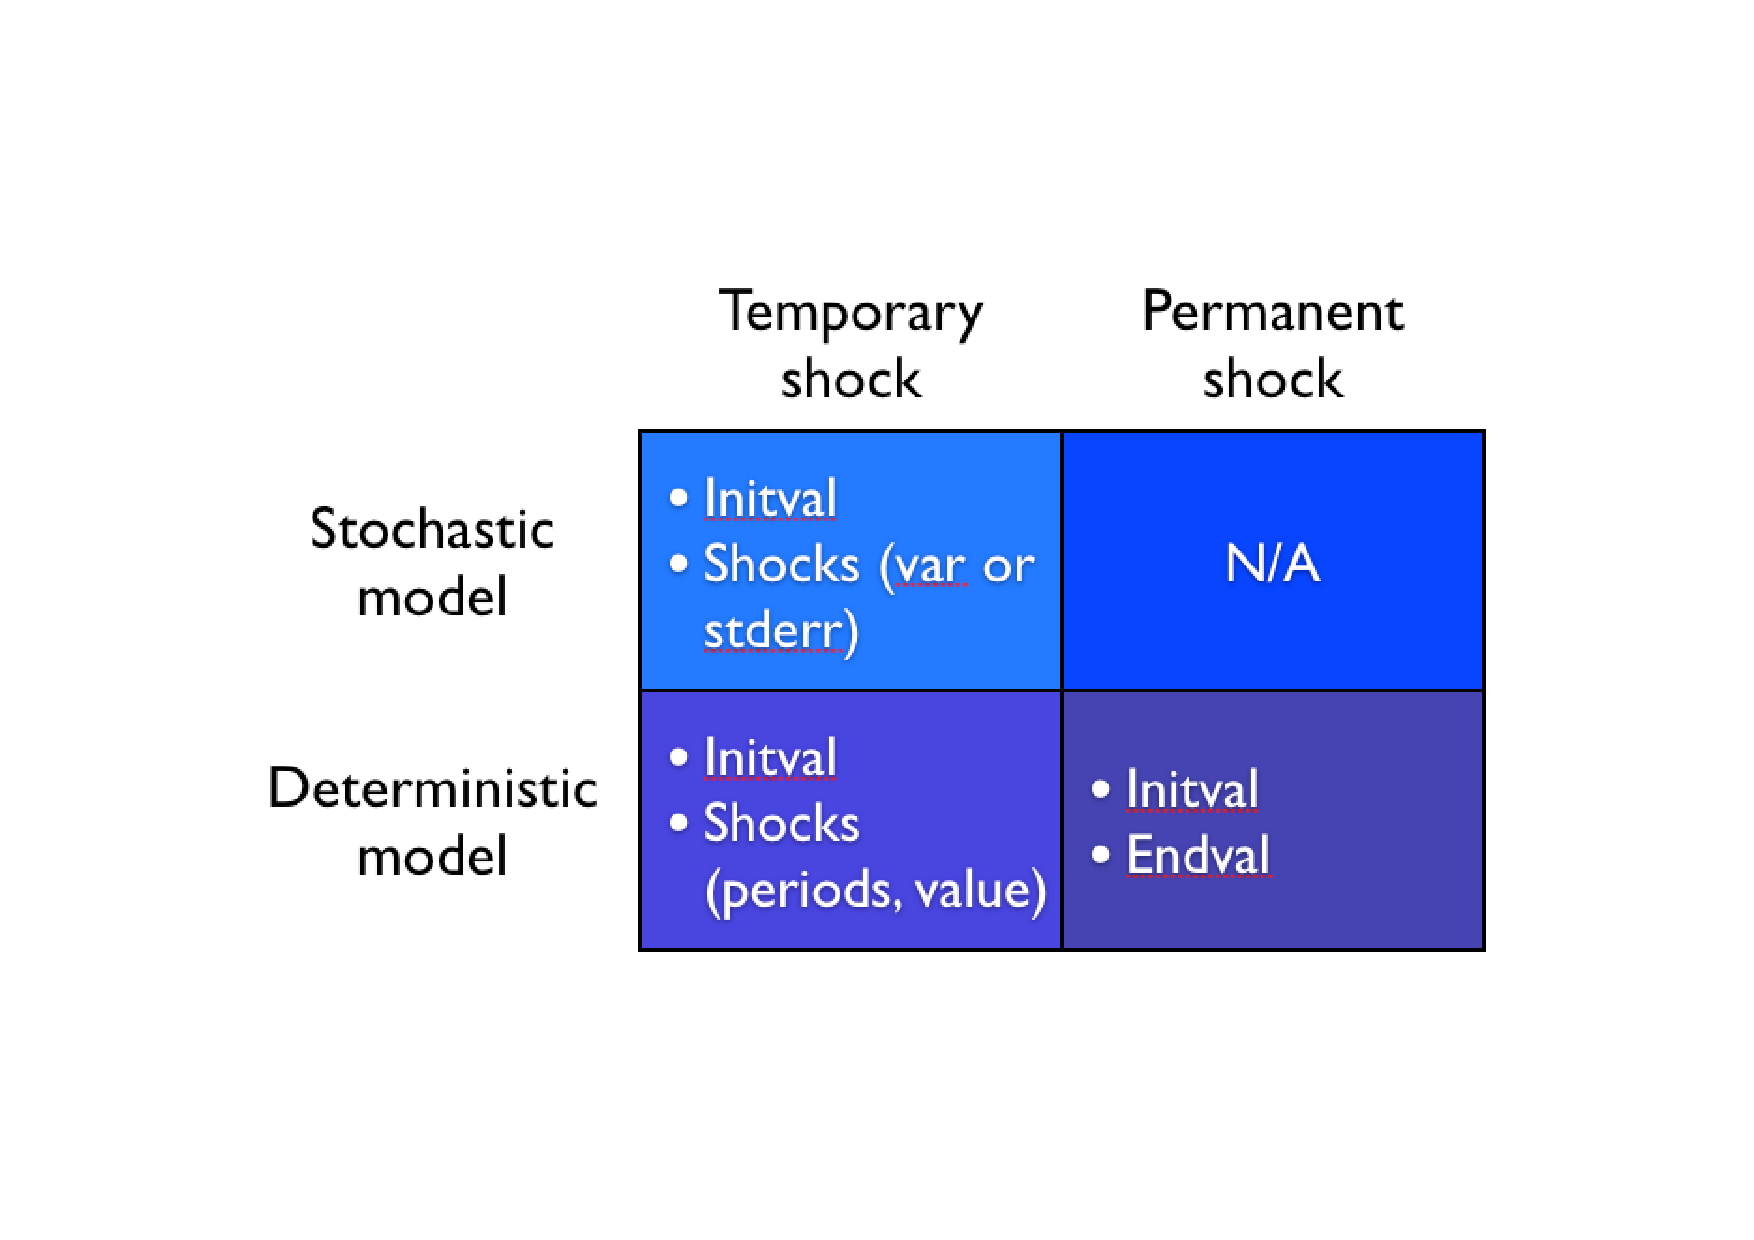
\includegraphics[width=1.0\textwidth]{P_ShockModel2} 
\end{center} 
\caption[Shock and model-type matrix]{Depending on the model type you're working with and the desired shocks, you will need to mix and match the various steady state and shock commands.} 
\end{figure}
\end{comment}

\subsection{Deterministic models - temporary shocks}
When working with a deterministic model, you have the choice of introducing both temporary and permanent shocks. The distinction is that under a temporary shock, the model eventually comes back to steady state, while under a permanent shock, the model reaches a new steady state. In both cases, though, the shocks are entirely expected, as explained in our original discussion on stochastic and deterministic models. \\

To work with a \textbf{temporary shock}, you are free to set the duration and level of the shock. To specify a shock that lasts 9 periods on $z_t$, for instance, you would write:\\
\\
\texttt{shocks;\\
var z;\\
periods 1:9;\\
values 0.1;\\
end;}\\

Given the above instructions, Dynare would replace the value of $z_t$ specified in the \texttt{initval} block with the value of 0.1 entered above. If variables were in logs, this would have corresponded to a 10\% shock. Note that you can also use the \texttt{mshocks} command which multiplies the initial value of an exogenous variable by the \texttt{mshocks} value. Finally, note that we could have entered future periods in the shocks block, such as \texttt{periods 5:10}, in order to study the anticipatory behavior of agents in response to future shocks.\\

\subsection{Deterministic models - permanent shocks}
To study the effects of a \textbf{permanent shock} hitting the economy today, such as a structural change in your model, you would not specify actual ``shocks'', but would simply tell the system to which (steady state) values you would like it to move and let Dynare calculate the transition path. To do so, you would use the \texttt{endval} block following the usual \texttt{initval} block. For instance, you may specify all values to remain common between the two blocks, except for the value of technology which you may presume changes permanently. The corresponding instructions would be:\\
\\
\texttt{initval;\\
  k = 9;\\
  c = 0.7;\\
  l = 0.3;\\
  w = 2.0;\\
  r = 0;\\
  z = 0; \\
end;\\
steady;\\
\\
endval;\\
  k = 9;\\
  c = 0.7;\\
  l = 0.3;\\
  w = 2.0;\\
  r = 0;\\
  z = 0.1; \\
end;\\
steady;}\\
\\
where \texttt{steady} can also be added to the \texttt{endval} block, and serves the same functionality as described earlier (namely, of telling Dynare to start and/ or end at a steady state close to the values you entered. If you do not use \texttt{steady} after \texttt{endval}, and the latter does not list exact steady state values, you may impose on your system that it does not return to steady state. This is unusual. In this case, your problem would become a so-called two boundary problem, which, when solved, requires that the path of your endogenous variables pass through the steady state closest to your \texttt{endval} values). In our example, we make use of the second \texttt{steady} since the actual terminal steady state values are bound to be somewhat different from those entered above, which are nothing but the initial values for all variables except for technology.\\

In the above example, the value of technology would move to 0.1 in period 1 (tomorrow) and thereafter. But of course, the other variables - the endogenous variables - will take longer to reach their new steady state values. \textsf{\textbf{TIP!}} If you instead wanted to study the effects of a permanent but future shock (anticipated as usual), you would have to add a \texttt{shocks} block after the \texttt{endval} block to ``undo'' the first several periods of the permanent shock. For instance, suppose you wanted the value of technology to move to 0.1, but only in period 10. Then you would follow the above \texttt{endval} block with:\\
\\
\texttt{shocks;\\
var z;\\
periods 1:9;\\
values 0;\\
end;}\\

\subsection{Stochastic models}

Recall from our earlier description of stochastic models that shocks are only allowed to be temporary. A permanent shock cannot be accommodated due to the need to stationarize the model around a steady state. Furthermore, shocks can only hit the system today, as the expectation of future shocks must be zero. With that in mind, we can however make the effect of the shock propagate slowly throughout the economy by introducing a ``latent shock variable'' such as $e_t$ in our example, that affects the model's true exogenous variable, $z_t$ in our example, which is itself an $AR(1)$, exactly as in the model we introduced from the outset. In that case, though, we would declare $z_t$ as an endogenous variable and $e_t$ as an exogenous variable, as we did in the preamble of the .mod file in section \ref{sec:preamble}. Supposing we wanted to add a shock with variance $\sigma^2$, where $\sigma$ is determined in the preamble block, we would write: \\
\\
\texttt{shocks;\\
var e = sigma\textasciicircum 2;\\
end;}\\
\\

\textsf{\textbf{TIP!}} You can actually \textbf{mix in deterministic shocks} in stochastic models by using the commands \texttt{varexo\_det} and listing some shocks as lasting more than one period in the \texttt{shocks} block. For information on how to do so, please see the \href{http://www.dynare.org/documentation-and-support/manual}{Reference Manual}. This can be particularly useful if you're studying the effects of anticipated shocks in a stochastic model. For instance, you may be interested in what happens to your monetary model if agents began expecting higher inflation, or a depreciation of your currency. \\

\section{Selecting a computation} \label{sec:compute}
So far, we have written an instructive .mod file, but what should Dynare do with it? What are we interested in? In most cases, it will be impulse response functions (IRFs) due to the external shocks. Let's see which are the appropriate commands to give to Dynare. Again, we will distinguish between deterministic and stochastic models. \\

\subsection{For deterministic models}
In the deterministic case, all you need to do is add the command \texttt{simul} at the bottom of your .mod file. Note that the command takes the option \mbox{\texttt{[ (periods=INTEGER) ] }} The command \texttt{simul} triggers the computation a numerical simulation of the trajectory of the model's solution for the number of periods set in the option. To do so, it uses a Newton method to solve simultaneously all the equations for every period (see \citet{Juillard1996} for details). Note that unless you use the \texttt{endval} command, the algorithm makes the simplifying assumption that the system is back to equilibrium after the specified number of periods. Thus, you must specify a large enough number of periods such that increasing it further doesn't change the simulation for all practical purpose. In the case of a temporary shock, for instance, the trajectory will basicaly describe how the system gets back to equilibrium after being perturbed from the shocks you entered.\\

\subsection{For stochastic models}
In the more common case of stochastic models, the command \texttt{stoch\_simul} is appropriate. This command instructs Dynare to compute a Taylor approximation of the decision and transition functions for the model (the equations listing current values of the endogenous variables of the model as a function of the previous state of the model and current shocks), impulse response 
functions and various descriptive statistics (moments, variance decomposition, correlation and autocorrelation coefficients).\footnote{For correlated shocks, the variance decomposition is computed as in the VAR literature through a Cholesky 
decomposition of the covariance matrix of the exogenous variables. When the shocks are correlated, the variance 
decomposition depends upon the order of the variables in the varexo command.}\\

Impulse response functions are the expected future path of the endogenous variables conditional on a shock in period 1 of one standard deviation.\textsf{\textbf{TIP!}} If you linearize your model up to a first order, impulse response functions are simply the algebraic forward iteration of your model's policy or decision rule. If you instead linearize to a second order, impulse response functions will be the result of actual Monte Carlo simulations of future shocks. This is because in second order linear equations, you will have cross terms involving the shocks, so that the effects of the shocks depend on the state of the system when the shocks hit. Thus, it is impossible to get algebraic average values of all future shocks and their impact. The technique is instead to pull future shocks from their distribution and see how they impact your system, and repeat this procedure a multitude of times in order to draw out an average response. That said, note that future shocks will not have a significant impact on your results, since they get averaged between each Monte Carlo trial and in the limit should sum to zero, given their mean of zero. Note that in the case of a second order approximation, Dynare will return the actual sample moments from the simulations. For first order linearizations, Dynare will instead report theoretical moments. In both cases, the return to steady state is asymptotic, \textsf{\textbf{TIP!}} thus you should make sure to specify sufficient periods in your IRFs such that you actually see your graphs return to steady state. Details on implementing this appear below.\\

If you're interested to peer a little further into what exactly is going on behind the scenes of Dynare's computations, have a look at Chapter \ref{ch:solbeh}. Here instead, we focus on the application of the command and reproduce below the most common options that can be added to \texttt{stoch\_simul}. For a complete list of options, please see the \href{http://www.dynare.org/documentation-and-support/manual}{Reference Manual}. \\

\textbf{Options following the \texttt{stoch\_simul} command:}
\begin{itemize}
\item ar = INTEGER: Order of autocorrelation coefficients to compute and to print (default = 5).
\item dr\_algo = 0 or 1: specifies the algorithm used for computing the quadratic approximation of the decision rules: $0$ uses a pure perturbation approach as in \citet{SchmittGrohe2004} (default) and 1 moves the point around which the Taylor expansion is computed toward the means of the distribution as in \citet{CollardJuillard2001a}.
\item drop = INTEGER: number of points dropped at the beginning of simulation before computing the summary 
statistics (default = 100).
\item hp\_filter = INTEGER: uses HP filter with lambda = INTEGER before computing moments (default: no filter).
\item hp\_ngrid = INTEGER: number of points in the grid for the discreet Inverse Fast Fourier Transform used in the 
HP filter computation. It may be necessary to increase it for highly autocorrelated processes (default = 512).
\item irf = INTEGER: number of periods on which to compute the IRFs (default = 40). Setting IRF=0, suppresses the 
plotting of IRF�s.  
\item relative\_irf requests the computation of normalized IRFs in percentage of the standard error of each shock.
\item nocorr: doesn�t print the correlation matrix (printing is the default).
\item nofunctions: doesn�t print the coefficients of the approximated solution (printing is the default). 
\item nomoments: doesn�t print moments of the endogenous variables (printing them is the default).
\item noprint: cancel any printing; usefull for loops. 
\item order = 1 or 2 : order of Taylor approximation (default = 2), unless you're working with a linear model in which case the order is automatically set to 1.  
\item periods = INTEGER: specifies the number of periods to use in simulations (default = 0). \textsf{\textbf{TIP!}} A simulation is similar to running impulse response functions with a model linearized to the second order, in the way that both sample shocks from their distribution to see how the system reacts, but a simulation only repeats the process once, whereas impulse response functions run a multitude of Monte Carlo trials in order to get an average response of your system. 
\item qz\_criterium = INTEGER or DOUBLE: value used to split stable from unstable eigenvalues in reordering the 
Generalized Schur decomposition used for solving 1st order problems (default = 1.000001).
\item replic = INTEGER: number of simulated series used to compute the IRFs (default = 1 if order = 1, and 50 
otherwise).
\item simul\_seed = INTEGER or DOUBLE or (EXPRESSION): specifies a seed for the random number generator so as to obtain the 
same random sample at each run of the program. Otherwise a different sample is used for each run (default: seed 
not specified). If you linearized to a second order, Dynare will actually undertake Monte Carlo simulations to generate moments of your variables. Because of the simulation, results are bound to be slightly different each time you run your program, except if you fix the seed for the random number generator. \textsf{\textbf{TIP!}} If you do decide to fix the seed, you should at least try to run your program without using \texttt{simul\_seed}, just to check the robustness of your results.
\end{itemize}

Going back to our good old example, suppose we were interested in printing all the various measures of moments of our variables, want to see impulse response functions for all variables, are basically happy with all default options and want to carry out simulations over a good number of periods. We would then end our .mod file with the following command:\\
\\
\texttt{stoch\_simul(periods=2100);}\\

\section{The complete .mod file}
For completion's sake, and for the pleasure of seeing our work bear its fruits, here are the complete .mod files corresponding to our example for the deterministic and stochastic case. You can find the corresponding files in the \textsl{models} folder under \textsl{UserGuide} in your installation of Dynare. The files are called \texttt{RBC\_Monop\_JFV.mod} for stochastic models and \texttt{RBC\_Monop\_Det.mod} for deterministic models. 

\subsection{The stochastic model}

\texttt{var y c k i l y\_l w r  z;\\
varexo e;\\
parameters beta psi delta alpha rho sigma epsilon;\\
alpha   = 0.33;\\
beta    = 0.99;\\
delta   = 0.023;\\
psi     = 1.75;\\
rho     = 0.95; \\ 
sigma   = (0.007\/(1-alpha));\\
epsilon = 10;\\
\\
model;\\
  (1/c) = beta*(1/c(+1))*(1+r(+1)-delta);\\
  psi*c/(1-l) = w;\\
  c+i = y;\\
  y = (k(-1)\textasciicircum alpha)*(exp(z)*l)\textasciicircum (1-alpha);\\
  w = y*((epsilon-1)/epsilon)*(1-alpha)/l;\\
  r = y*((epsilon-1)/epsilon)*alpha/k(-1);\\
  i = k-(1-delta)*k(-1);\\
  y\_l = y/l;\\
  z = rho*z(-1)+e;\\
end;\\
\\
initval;\\
  k = 9;\\
  c = 0.7;\\
  l = 0.3;\\
  w = 2.0;\\
  r = 0;\\
  z = 0; \\
  e = 0;\\
end;\\
\\
steady;\\
\\
check;\\
\\
shocks;\\
var e = sigma\textasciicircum 2;\\
end;\\
\\
stoch\_simul(periods=2100);}\\

\subsection{The deterministic model (case of temporary shock)}

\texttt{var y c k i l y\_l w r ;\\
varexo z;\\
parameters beta psi delta alpha sigma epsilon;\\
alpha   = 0.33;\\
beta    = 0.99;\\
delta   = 0.023;\\
psi     = 1.75;\\
sigma   = (0.007\/(1-alpha));\\
epsilon = 10;\\
\\
model;\\
  (1/c) = beta*(1/c(+1))*(1+r(+1)-delta);\\
  psi*c/(1-l) = w;\\
  c+i = y;\\
  y = (k(-1)\textasciicircum alpha)*(exp(z)*l)\textasciicircum (1-alpha);\\
  w = y*((epsilon-1)/epsilon)*(1-alpha)/l;\\
  r = y*((epsilon-1)/epsilon)*alpha/k(-1);\\
  i = k-(1-delta)*k(-1);\\
  y\_l = y/l;\\
end;\\
\\
initval;\\
  k = 9;\\
  c = 0.7;\\
  l = 0.3;\\
  w = 2.0;\\
  r = 0;\\
  z = 0; \\
end;\\
\\
steady;\\
\\
check;\\
\\
shocks;\\
var z;
periods 1:9;\\
values 0.1;\\
end;\\
\\
simul(periods=2100);}\\

\section{File execution and results}
To see this all come to life, let's run our .mod file, which is conveniently installed by default in the Dynare ``examples'' directory (the .mod file corresponding to the stochastic model is called RBC\_Monop\_JFV.mod and that corresponding to the deterministic model is called RBC\_Monop\_Det.mod). (** note, this may not be the case when testing the beta version of Matlab version 4) \\

\textbf{To run a .mod file}, navigate within Matlab to the directory where the example .mod files are stored. You can do this by clicking in the ``current directory'' window of Matlab, or typing the path directly in the top white field of Matlab. Once there, all you need to do is place your cursor in the Matlab command window and type, for instance, \texttt{dynare ExSolStoch;} to execute your .mod file. \\

Running these .mod files should take at most 30 seconds. As a result, you should get two forms of output - tabular in the Matlab command window and graphical in one or more pop-up windows. Let's review these results.\\

\subsection{Results - stochastic models}
\textbf{The tabular results} can be summarized as follows:
\begin{enumerate}
\item \textbf{Model summary:} a count of the various variable types in your model (endogenous, jumpers, etc...).
\item \textbf{Eigenvalues} should be displayed, and you should see a confirmation of the Blanchard-Kahn conditions if you used the command \texttt{check} in your .mod file. 
\item \textbf{Matrix of covariance of exogenous shocks:} this should square with the values of the shock variances and co-variances you provided in the .mod file.
\item \textbf{Policy and transition functions:} Solving the rational exectation model, $\mathbb{E}_t[f(y_{t+1},y_t,y_{t-1},u_t)]=0$ , means finding an unkown function, $y_t = g(y_{t-1},u_t)$  that could be plugged into the original model and satisfy the implied restrictions (the first order conditions). A first order approximation of this function can be written as $y_t = \bar{y} + g_y \hat{y}_{t-1} + g_u u_t$, with $\hat{y}_t = y_t-\bar{y}$ and $\bar{y}$ being the steadystate value of $y$, and where $g_x$ is the partial derivative of the $g$ function with respect to variable $x$. In other words, the function $g$ is a time recursive (approximated) representation of the model that can generate timeseries that will approximatively satisfy the rational expectation hypothesis contained in the original model. In Dynare, the table ``Policy and Transition function'' contains the elements of $g_y$ and $g_u$. Details on the policy and transition function can be found in Chapter \ref{ch:estadv}.
\item \textbf{Moments of simulated variables:} up to the fourth moments.
\item \textbf{Correlation of simulated variables:} these are the contemporaneous correlations, presented in a table.
\item \textbf{Autocorrelation of simulated variables:} up to the fifth lag, as specified in the options of \texttt{stoch\_simul}. 
\end{enumerate}

\textbf{The graphical results}, instead, show the actual impulse response functions for each of the endogenous variables, given that they actually moved. These can be especially useful in visualizing the shape of the transition functions and the extent to which each variable is affected. \textsf{\textbf{TIP!}} If some variables do not return to their steady state, either check that you have included enough periods in your simulations, or make sure that your model is stationary, i.e. that your steady state actually exists and is stable. If not, you should detrend your variables and rewrite your model in terms of those variables. 

\subsection{Results - deterministic models}
Automatically displayed results are much more scarce in the case of deterministic models. If you entered \texttt{steady}, you will get a list of your steady state results. If you entered \texttt{check}, eigenvalues will also be displayed and you should receive a statement that the rank condition has been satisfied, if all goes well! Finally, you will see some intermediate output: the errors at each iteration of the Newton solver used to estimate the solution to your model. \textsf{\textbf{TIP!}} You should see these errors decrease upon each iteration; if not, your model will probably not converge. If so, you may want to try to increase the periods for the transition to the new steady state (the number of simulations periods). But more often, it may be a good idea to revise your equations. Of course, although Dynare does not display a rich set of statistics and graphs corresponding to the simulated output, it does not mean that you cannot create these by hand from Matlab. To do so, you should start by looking at section \ref{sec:FindOut} of chapter \ref{ch:soladv} on finding, saving and viewing your output. 












\chapter{Solving DSGE models - advanced topics} \label{ch:soladv}

This chapter is a collection of topics - not all related to each other - that you will probably find interesting or at least understandable, if you have read, and/ or feel comfortable with, the earlier chapter \ref{ch:solbase} on the basics of solving DSGE models. To provide at least some consistency, this chapter is divided into three sections. \textbf{The first section} deals directly with features of Dynare, such as dealing with correlated shocks, finding and saving your output, using loops, referring to external files and dealing with infinite eigenvalues. \textbf{The second section} overviews some of the inner workings of Dynare. The goal is to provide a brief explanation of the files that are created by Dynare to help you in troubleshooting or provide a starting point in case you actually want to customize the way Dynare works.  \textbf{The third section} of the chapter focusses on modeling tips optimized for Dynare, but possibly also helpful for other work.\\

\section{Dynare features and functionality}

\subsection{Other examples}
Other examples of .mod files used to generate impulse response functions are available on the Dynare website. In particular, Jesus Fernandez-Villaverde has provided a series of RBC model variants (from the most basic to some including variable capacity utilization, indivisible labor and investment specific technological change). You can find these, along with helpful notes and explanations, in the \href{http://www.dynare.org/documentation-and-support/examples}{Official Examples} section of the Dynare website.\\

Also, don't forget to check occasionally the \href{http://www.dynare.org/phpBB3}{Dynare contributions and examples forum} to see if any other user has posted an example that could help you in your work; or maybe you would like to post an example there yourself?

\subsection{Alternative, complete example}
The following example aims to give you an alternative example to the one in chapter \ref{ch:solbase}, to learn the workings of Dynare. It also aims to give you exposure to dealing with \textbf{several correlated shocks}. Your model may have two or more shocks, and these may be correlated to each other. The example below illustrates how you would introduce this into Dynare.  Actually, the example provided is somewhat more complete than strictly necessary. This is to give you an alternative, full-blown example to the one described in chapter \ref{ch:solbase}.

\subsubsection{The model}
The model is a simplified standard RBC model taken from \citet{CollardJuillard2003} which served as the original User Guide for Dynare. \\

The economy consists of an infinitely living representative agent who values consumption $c_t$ and labor services $h_t$ according to the following utility function
\[
\mathbb{E}_t \sum_{\tau=t}^\infty \beta^{\tau-t} \left( \log (c_t) - \theta \frac{h_t^{1+\psi}}{1+\psi} \right)
\] 
where, as usual, the discount factor $0<\beta<1$, the disutility of labor $\theta > 0$ and the labor supply elasticity $\psi \geq 0$. \\

A social planner maximizes this utility function subject to the resource constraint
\[
c_t + i_t = y_t
\]
where $i_t$ is investment and $y_t$ output. Consumers are therefore also owners of the firms. The economy is a real economy, where part of output can be consumed and part invested to form physical capital. As is standard, the law of motion of capital is given by
\[
k_{t+1} = \exp (b_t)i_t + (1-\delta)k_t
\]
with $0<\delta<1$, where $\delta$ is physical depreciation and $b_t$ a shock affecting incorporated technological progress. \\

We assume output is produced according to a standard constant returns to scale technology of the form
\[
y_t = \exp (a_t)k_t^\alpha h_t^{1-\alpha}
\]
with $\alpha$ being the capital elasticity in the production function, with $0<\alpha<1$, and where $a_t$ represents a stochastic technological shock (or Solow residual). \\

Finally, we specify a \textbf{shock structure} that allows for shocks to display persistence across time and correlation in the current period. That is
\[
\left( \begin{array}{c}a_t \\
b_t \end{array} \right) = \left( \begin{array}{c c} \rho & \tau \\
\tau & \rho \end{array} \right) \left( \begin{array}{c}a_{t-1} \\
b_{t-1} \end{array} \right) + \left( \begin{array}{c}\epsilon_t \\
\nu_t \end{array} \right)
\]
where $|\rho + \tau|<1$ and $|\rho - \tau|<1$ to ensure stationarity (we call $\rho$ the coefficient of persistence and $\tau$ that of cross-persistence). Furthermore, we assume $\mathbb{E}_t (\epsilon_t)=0$, $\mathbb{E}_t (\nu_t)=0$ and that the contemporaneous variance-covariance matrix of the innovations $\epsilon_t$ and $\nu_t$ is given by
\[
\left( \begin{array}{c c} \sigma_\epsilon^2 & \psi \sigma_\epsilon \sigma_\nu \\
\psi \sigma_\epsilon \sigma_\nu & \sigma_\nu^2 \end{array} \right)
\]
and where $corr(\epsilon_t \nu_s)=0$, $corr(\epsilon_t \epsilon_s)=0$ and $corr(\nu_t \nu_s)=0$ for all $t \neq s$. \\

This system - probably quite similar to standard RBC models you have run into - yields the following first order conditions (which are straightforward to reproduce in case you have doubts\ldots) and equilibrium conditions drawn from the description above. Note that the first equation captures the labor supply function and the second the intertemporal consumption Euler equation.
\[
\begin{aligned}
c_t \theta h_t^{1+\psi} = (1-\alpha)y_t \\
1= \beta \mathbb{E}_t \left[ \left( \frac{\exp(b_t)c_t}{\exp(b_{t+1})c_{t+1}} \right) \left( \exp(b_{t+1}) \alpha \frac{y_{t+1}}{k_{t+1}}+1-\delta \right) \right] \\
y_t = \exp (a_t)k_t^\alpha h_t^{1-\alpha} \\
k_{t+1} = \exp (b_t)i_t + (1-\delta)k_t \\
a_t = \rho a_{t-1} + \tau b_{t-1} + \epsilon_t \\
b_t = \tau a_{t-1} + \rho b_{t-1} + \nu_t
\end{aligned}
\] 

\subsubsection{The .mod file}
To ``translate'' the model into a language understandable by Dynare, we would follow the steps outlined in chapter \ref{ch:solbase}. We will assume that you're comfortable with these and simply present the final .mod file below. Fist, though, note that to introduce shocks into Dynare, we have two options (this was not discussed in the earlier chapter). Either write:\\
\\
\texttt{shocks;\\
var e; stderr 0.009;\\
var u; stderr 0.009;\\
var e, u = phi*0.009*0.009;\\
end;}\\
\\
where the last line specifies the contemporaneous correlation between our two exogenous variables. \\

Alternatively, you can also write: \\
\\
\texttt{shocks;\\
var e = 0.009\textasciicircum 2;\\
var u = 0.009\textasciicircum 2;\\
var e, u = phi*0.009*0.009;\\
end;}\\

So that you can gain experience by manipulating the entire model, here is the complete .mod file corresponding to the above example. You can find the corresponding file in the \textsl{models} folder under \textsl{UserGuide} in your installation of Dynare. The file is called \textsl{Alt\_Ex1.mod}. \\
\\
\\
\texttt{var y, c, k, a, h, b;\\
varexo e, u;\\
parameters beta, rho, alpha, delta, theta, psi, tau;\\
\\
alpha = 0.36;\\
rho   = 0.95;\\
tau   = 0.025;\\
beta  = 0.99;\\
delta = 0.025;\\
psi   = 0;\\
theta = 2.95;\\
\\
phi   = 0.1;\\
\\
model;\\
c*theta*h\textasciicircum (1+psi)=(1-alpha)*y;\\
k = beta*(((exp(b)*c)/(exp(b(+1))*c(+1)))\\
    *(exp(b(+1))*alpha*y(+1)+(1-delta)*k));\\
y = exp(a)*(k(-1)\textasciicircum alpha)*(h\textasciicircum (1-alpha));\\
k = exp(b)*(y-c)+(1-delta)*k(-1);\\
a = rho*a(-1)+tau*b(-1) + e;\\
b = tau*a(-1)+rho*b(-1) + u;\\
end;\\
\\
initval;\\
y = 1.08068253095672;\\
c = 0.80359242014163;\\
h = 0.29175631001732;\\
k = 5;\\
a = 0;\\
b = 0;\\
e = 0;\\
u = 0;\\
end;\\
\\
shocks;\\
var e; stderr 0.009;\\
var u; stderr 0.009;\\
var e, u = phi*0.009*0.009;\\
end;\\
\\
stoch\_simul(periods=2100);}\\

\subsection{Finding, saving and viewing your output} \label{sec:FindOut}
Where is output stored? Most of the moments of interest are stored in global variable \texttt{oo\_} You can easily browse this global variable in Matlab by either calling it in the command line, or using the workspace interface. In global variable \texttt{oo\_} you will find the following (\textsf{\textbf{NOTE!}} variables will always appear in the order in which you declared them in the preamble block of your .mod file):
\begin{itemize}
\item \texttt{steady\_state}: the steady state of your variables
\item \texttt{mean}: the mean of your variables
\item \texttt{var}: the variance of your variables
\item \texttt{autocorr}: the various autocorrelation matrices of your variables. Each row of these matrices will correspond to a variables in time $t$, and columns correspond to the variables lagged 1, for the first matrix, then lagged 2 for the second matrix, and so on. Thus, the matrix of autocorrelations that is automatically displayed in the results after running \texttt{stoch\_simul} has, running down each column, the diagonal elements of each of the various autocorrelation matrices described here. 
\item \texttt{gamma\_y}: the matrices of autocovariances. \texttt{gamma\_y\{1\}} represents variances, while \texttt{gamma\_y\{2\}} represents autocovariances where variables on each column are lagged by one period and so on. By default, Dynare will return autocovariances with a lag of 5. The last matrix (\texttt{gamma\_y\{7\}} in the default case) returns the \textbf{variance decomposition}, where each column captures the independent contribution of each shock to the variance of each variable. 
\end{itemize}

Furthermore, if you decide to run impulse response functions, you will find a global variable \texttt{oo\_.irfs} comprising of vectors named \texttt{endogenous variable\_exogenous variable}, like \texttt{y\_e}, reporting the values of the endogenous variables corresponding to the impulse response functions, as a result of the independent impulse of each exogenous shock. \\

To save your simulated variables, you can add the following command at the end of your .mod file: \texttt{dynasave (FILENAME) [variable names separated by commas]} If no variable names are specified in the optional field, Dynare will save all endogenous variables. In Matlab, variables saved with the \texttt{dynasave} command can be retrieved by using the Matlab command \texttt{load -mat FILENAME}.

\subsection{Referring to external files}
You may find it convenient to refer to an external file, either to compute the steady state of your model, or when specifying shocks in an external file. The former is described in section \ref{sec:ssshock} of chapter \ref{ch:solbase} when discussing steady states. The advantage of using Matlab, say, to find your model's steady state was clear with respect to Dynare version 3, as the latter resorted to numerical approximations to find steady state values. But Dynare version 4 now uses the same analytical methods available in Matlab. For most usage scenarios, you should therefore do just as  well to ask Dynare to compute your model's steady state (except, maybe, if you want to run loops, to vary your parameter values, for instance, in which case writing a Matlab program may be more handy).\\

But you may also be interested in the second possibility described above, namely of specifying shocks in an external file, to simulate a model based on shocks from a prior estimation, for instance. You could then retrieve the exogenous shocks from the oo\_ file by saving them in a file called datafile.mat. Finally, you could simulate a deterministic model with the shocks saved from the estimation by specifying the source file for the shocks, using the \\ \mbox{\texttt{shocks(shocks\_file = datafile.mat)}} command.
But of course, this is a bit of a workaround, since you could also use the built-in commands in Dynare to generate impulse response functions from estimated shocks, as described in chapter \ref{ch:estbase}. \\

\subsection{Infinite eigenvalues}
If you use the command \texttt{check} in your .mod file, Dynare will report your system's eigenvalues and tell you if these meet the Blanchard-Kahn conditions. At that point, don't worry if you get infinite eigenvalues - these are are firmly grounded in the theory of generalized eigenvalues. They have no detrimental influence on the solution algorithm. As far as Blanchard-Kahn conditions are concerned infinite eigenvalues are counted as explosive roots of modulus larger than one. \\

\section{Files created by Dynare} \label{sec:dynfiles}
At times, you may get a message that there is an error in a file with a new name, or you may want to have a closer look at how Dynare actually solves your model - out of curiosity or maybe to do some customization of your own. You may therefore find it helpful to get a brief overview of the internal files that Dynare generates and the function of each one. \\

The dynare pre-processors essentially does three successive tasks:
(i) parsing of the mod file (it checks that the mod file is syntactically
correct), and its translation into internal machine representation (in
particular, model equations are translated into expression trees), (ii) symbolic derivation of the model equations, up to the needed order
(depending on the computing needs), (iii) outputting of several files, which are used from matlab. If the mod
file is ``filename.mod", then the pre-processor creates the following
files:

\begin{itemize}
\item \textbf{filename.m}: a matlab file containing several instructions, notably
the parameter initializations and the matlab calls corresponding to
computing tasks
\item \textbf{filename\_dynamic.m}: a matlab file containing the model equations and
their derivatives (first, second and maybe third).
    Endogenous variables (resp. exogenous variables, parameters) are
contained in a ``y" (resp. ``x", ``params") vector, with an index number
depending on the declaration order.
    The ``y" vector has as many entries as their are (variable, lag)
pairs in the declared model.
    The model equations residuals are stored in a vector named
``residuals".
    The model jacobian is put in ``g1" matrix. Second (resp. third)
derivatives are in ``g2" matrix (resp. ``g3").
    If the ``use\_dll" option has been specified in the model declaration,
the pre-processor will output a C file (with .c extension) rather than a
matlab file. It is then compiled to create a library (DLL) file. Using a
compiled C file is supposed to give better computing performance in
model simulation/estimation.
\item \textbf{filename\_static.m}: a matlab file containing the stationarized
version of the model (i.e. where lagged variables are replaced by
current variables), with its jacobian. Used to compute the steady state.
Same notations than the dynamic file. Replaced by a C file when
``use\_dll" option is specified.
\end{itemize}

\section{Modeling tips}

\subsection{Stationarizing your model}
Models in Dynare must be stationary, such that you can linearize them around a steady state and return to steady state after a shock. Thus, you must first stationarize your model, then linearize it, either by hand, or by letting Dynare do the work.  You can then reconstruct ex-post the non-stationary simulated variables after running impulse response functions.\\

For deterministic models, the trick is to use only stationary variables in $t+1$. More generally, if $y_t$ is $I(1)$, you can always write $y_{t+1}$ as $y_t+dy_{t+1}$, where $dy_t= y_t-y_{t-1}$. Of course, you need to know the value of $dy_t$ at the final equilibrium.\\

Note that in a stationary model, it is expected that variables will eventually go back to steady state after the initial shock. If you expect to see a growing curve for a variable, you are thinking about a growth model. Because growth models are nonstationary, it is easier to work with the stationarized version of such models. Again, if you know the trend, you can always add it back after the simulation of the stationary components of the variables. 

\subsection{Expectations taken in the past}
For instance, to enter the term $\mathbb{E}_{t-1}y_t$, define $s_t=\mathbb{E}_t[y_{t+1}]$ and then use $s(-1)$ in your .mod file. Note that, because of Jensen's inequality, you cannot do this for terms that enter your equation in a non-linear fashion. If you do have non-linear terms on which you want to take expectations in the past, you would need to apply the above manipulation to the entire equation, as if $y_t$ were an equation, not just a variable.

\subsection{Infinite sums}

Dealing with infinite sums is tricky in general, and needs particular care when working with Dynare. The trick is to use a \textbf{recursive
representation} of the sum. For example, suppose your model included:
\[\sum^{\infty}_{j=0}\beta^j x_{t+j}=0, \]

Note that the above can also be written by using an auxiliary variable $S_t$, defined as:
\[S_t\equiv \sum^{\infty}_{j=0}\beta^j x_{t+j},\]
which can also be written in the following recursive manner:
\[S_t\equiv \sum^{\infty}_{j=0}\beta^j x_{t+j}=x_t +\sum^{\infty}_{j=1}\beta^j
x_{t+j}=x_t+\beta\sum^{\infty}_{j=0}\beta^j x_{t+1+j} \equiv x_t + S_{t+1}\]

This formulation turns out to be useful in problems of the following
form:

\[\sum^{\infty}_{j=0}\beta^j x_{t+j}=p_t\sum^{\infty}_{j=0}\gamma^j y_{t+j}, \]
which can be written as a recursive system of the form:
\[S1_t=x_t+\beta S1_{t+1},\]
\[S2_t=y_t+\gamma S2_{t+1},\]
\[S1=p_t S2.\]

This is particularly helpful, for instance, in a \textbf{Calvo type setting}, as illustrated in the following brief example. The RBC model with monopolistic competition introduced in chapter \ref{ch:solbase} involved flexible prices. The extension with sticky prices, � la Calvo for instance, is instead typical of the new Keynesian monetary literature, exemplified by papers such as \citet{ClaridaGaliGertler1999}. \\

The optimal price for a firm resetting its price in period $t$, given that it will be able to reset its price only with probability $1-\theta$ each  period, is
\[
p_t^*(i) = \mu + (1-\beta \theta) \sum_{k=0}^\infty (\beta \theta)^k \mathbb{E}_t [mc_{t+k}^n (i)]
\]
where $\mu$ is the markup, $\beta$ is a discount factor, $i$ represents a firm of the continuum between 0 and 1, and $mc_t$ is marginal cost as described in the example in chapter \ref{ch:solbase}. The trouble, of course, is \textbf{how to input this infinite sum into Dynare}? \\

It turns out that the Calvo price setting implies that the aggregate price follows the equation of motion $p_t = \theta p_{t-1} + (1-\theta) p_t^*$, thus implying the following inflation relationship $\pi_t = (1-\theta) (p_t^* - p_{t-1})$. Finally, we can also rewrite the optimal price setting equation, after some algebraic manipulations, as
\[
p_t^* - p_{t-1} = (1-\beta \theta) \sum_{k=0}^\infty (\beta \theta)^k \mathbb{E}_t [\widehat{mc}_{t+k}] + \sum_{k=0}^\infty (\beta \theta)^k \mathbb{E}_t [\pi_{t+k}]
\]
where $\widehat{mc}_{t+k} = mc_{t+k} + \mu$ is the deviation of the marginal cost from its natural rate, defined as the marginal cost when prices are perfectly flexible. \\

The trick now is to note that the above can be written recursively, by writing the right hand side as the first term of the sum (with $k=0$) plus the remainder of the sum, which can be written as the left hand side term scrolled forward one period and appropriately discounted. Mathematically, this yields:
\[
p_t^* - p_{t-1} =�(1-\beta \theta) \widehat{mc}_{t+k} + \pi_t + \beta�\theta \mathbb{E}_t [p_{t+1}^* - p_t]
\]
which has gotten rid of our infinite sum! That would be enough for Dynare, but for convenience, we can go one step further and write the above as
\[
\pi_t = \beta \mathbb{E}_t [\pi_{t+1}] + \lambda \widehat{mc}_{t}
\]
where $\lambda \equiv \frac{(1-\theta)(1-\beta\theta)}{\theta}$, which is the recognizable inflation equation in the new Keynesian (or new Neoclassical) monetary literature. 

\subsection{Infinite sums with changing timing of expectations}

When you are not able to write an infinite sum recursively, as the index of the expectations changes with each element of the sum, as in the following example, a different approach than the one mentioned above is necessary. \\

Suppose your model included the following sum: 
\[
y_t=\sum_{j=0}^{\infty} \mathbb{E}_{t-j}x_t
\]
where $y_t$ and $x_t$ are endogenous variables. \\

In Dynare, the best way to handle this is to write out the first $k$ terms explicitly and enter each one in Dynare, such as: $\mathbb{E}_{t-1}x_t + \mathbb{E}_{t-2}x_t+\ldots + \mathbb{E}_{t-k}x_t$.

\chapter{Estimating DSGE models - basics} \label{ch:estbase}

As in the chapter \ref{ch:solbase}, this chapter is structured around an example. The goal of this chapter is to lead you through the basic functionality in Dynare to estimate models using Bayesian techniques, so that by the end of the chapter you should have the capacity to estimate a model of your own. This chapter is therefore very practically-oriented and abstracts from the underlying computations that Dynare undertakes to estimate a model; that subject is instead covered in some depth in chapter \ref{ch:estbeh}, while more advanced topics of practical appeal are discussed in chapter \ref{ch:estadv}. \\

\section{Introducing an example} \label{sec:modsetup}
The example introduced in this chapter is particularly basic. This is for two reasons. First, we did not want to introduce yet another example in this section; there's enough new material to keep you busy. Instead, we thought it would be easiest to simply continue working with the example introduced in chapter \ref{ch:solbase} with which you are probably already quite familiar. Second, the goal of the example in this chapter is really to explain features in context, but not necessarily to duplicate a ``real life scenario'' you would face when writing a paper. Once you feel comfortable with the content of this chapter, though, you can always move on to chapter \ref{ch:estadv} where you will find a full-fledged replication of a recent academic paper, featuring a non-stationary model. \\

Recall from chapter \ref{ch:solbase} that we are dealing with an RBC model with monopolistic competition. Suppose we had data on business cycle variations of output. Suppose also that we thought our little RBC model did a good job of reproducing reality. We could then use Bayesian methods to estimate the parameters of the model: $\alpha$, the capital share of output, $\beta$, the discount factor, $\delta$, the depreciation rate, $\psi$, the weight on leisure in the utility function, $\rho$, the degree of persistence in productivity, and $\epsilon$, the markup parameter. Note that in Bayesian estimation, the condition for undertaking estimation is that there be at least as many shocks as there are observables (a less stringent condition than for maximum likelihood estimation). It may be that this does not allow you to identify all your parameters - yielding posterior distributions identical to prior distributions - but the Bayesian estimation procedure would still run successfully. Let's see how to go about doing this. 

\section{Declaring variables and parameters}
To input the above model into Dynare for estimation purposes, we must first declare the model's variables in the preamble of the .mod file. This is done exactly as described in chapter \ref{ch:solbase} on solving DSGE models. We thus begin the .mod file with:\\
\\
\texttt{var y c k i l y\_l w r  z;\\
varexo e;\\
\\
parameters beta psi delta alpha rho epsilon;\\}\\
\\

\section{Declaring the model}
Suppose that the equation of motion of technology is a \textbf{stationary} AR(1) with an autoregressive parameter, $\rho$, less than one. The model's variables would therefore be stationary and we can proceed without complications. The alternative scenario with \textbf{non-stationary variables} is more complicated and dealt with in chapter \ref{ch:estadv} (in the additional example). In the stationary case, our model block would look exactly as in chater \ref{ch:solbase}:\\
\\
\texttt{model;\\
  (1/c) = beta*(1/c(+1))*(1+r(+1)-delta);\\
  psi*c/(1-l) = w;\\
  c+i = y;\\
  y = (k(-1)$\hat{}$alpha)*(exp(z)*l)$\hat{}$(1-alpha);\\
  w = y*((epsilon-1)/epsilon)*(1-alpha)/l;\\
  r = y*((epsilon-1)/epsilon)*alpha/k(-1);\\
  i = k-(1-delta)*k(-1);\\
  y\_l = y/l;\\
  z = rho*z(-1)+e;\\
end;}\\
\\

\section{Declaring observable variables}
This should not come as a surprise. Dynare must know which variables are observable for the estimation procedure. \textsf{\textbf{NOTE!}} These variables must be available in the data file, as explained in section \ref{sec:estimate} below. For the moment, we write:\\
\\
\texttt{varobs Y;}\\

\section{Specifying the steady state}
Before Dynare estimates a model, it first linearizes it around a steady state. Thus, a steady state must exist for the model and although Dynare can calculate it, we must give it a hand by declaring approximate values for the steady state. This is just as explained in details and according to the same syntax outlined in chapter \ref{ch:solbase}, covering the \texttt{initval}, \texttt{steady} and \texttt{check} commands. In fact, as this chapter uses the same model as that outlined in chapter \ref{ch:solbase}, the steady state block will look exactly the same.\\

\textsf{\textbf{TIP!}} During estimation, in finding the posterior mode, Dynare recalculates the steady state of the model at each iteration of the optimization routine (more on this later), based on the newest round of parameters available. Thus, by providing approximate initial values and relying solely on the built-in Dynare algorithm to find the steady state (a numerical procedure), you will significantly slow down the computation of the posterior mode. Dynare will end up spending 60 to 70\% of the time recalculating steady states. It is much more efficient to write an external \textbf{Matlab steady state file} and let Dynare use that file to find the steady state of your model by algebraic procedure. For more details on writing an external Matlab file to find your model's steady state, please refer to section \ref{sec:findsteady} of chapter \ref{ch:solbase}. \\


\section{Declaring priors}
Priors play an important role in Bayesian estimation and consequently deserve a central role in the specification of the .mod file. Priors, in Bayesian estimation, are declared as a distribution. The general syntax to introduce priors in Dynare is the following:\\
\\
\texttt{estimated\_params;\\
PARAMETER NAME, PRIOR\_SHAPE, PRIOR\_MEAN, PRIOR\_STANDARD\_ERROR [, PRIOR 3$^{\textrm{rd}}$ PARAMETER] [,PRIOR 4$^{\textrm{th}}$ PARAMETER] ; \\
end; }\\
\\
where the following table defines each term more clearly\\
\\
    \begin{tabular}{llc}
    \textbf{\underline{PRIOR\_SHAPE}} & \textbf{\underline{Corresponding distribution}} & \textbf{\underline{Range}} \\
      NORMAL\_PDF & $N(\mu,\sigma)$ & $\mathbb{R}$\\
      GAMMA\_PDF &  $G_2(\mu,\sigma,p_3)$ & $[p_3,+\infty)$\\
        BETA\_PDF & $B(\mu,\sigma,p_3,p_4)$ & $[p_3,p_4]$\\
        INV\_GAMMA\_PDF & $IG_1(\mu,\sigma)$ & $\mathbb R^+$\\
UNIFORM\_PDF& $U(p_3,p_4)$ &  $[p_3,p_4]$
    \end{tabular}\\
    \\
    \\
    where $\mu$ is the \texttt{PRIOR\_MEAN}, $\sigma$ is the \texttt{PRIOR\_STANDARD\_ERROR}, $p_3$ is the \texttt{PRIOR 3$^{\textrm{rd}}$ PARAMETER} (whose default is 0) and $p_4$ is the \texttt{PRIOR 4$^{\textrm{th}}$ PARAMETER} (whose default is 1).  \textsf{\textbf{TIP!}} When specifying a uniform distribution between 0 and 1 as a prior for a parameter, say $\alpha$, you therefore have to put two empty spaces for parameters $\mu$ and $\sigma$, and then specify parameters $p3$ and $p4$, since the uniform distribution only takes $p3$ and $p4$ as arguments. For instance, you would write \texttt{alpha, uniform\_pdf, , , 0,1;} \\
    
For a more complete review of all possible options for declaring priors, as well as the syntax to declare priors for maximum likelihood estimation (not Bayesian), see the \href{http://www.cepremap.cnrs.fr/juillard/mambo/index.php?option=com_content&task=view&id=51&Itemid=84}{Reference Manual}. Note also that if some parameters in a model are calibrated and are not to be estimated, you should declare them as such, by using the \texttt{parameters} command and its related syntax, as explained in chapter \ref{ch:solbase}. \\

\textsf{\textbf{TIP!}} Choosing the appropriate prior for your parameters is a tricky, yet very important endeavor. It is worth spending time on your choice of priors and to test the robustness of your results to your priors. Some considerations may prove helpful. First, think about the domain of your prior over each parameter. Should it be bounded? Should it be opened on either or both sides? Remember also that if you specify a probability of zero over a certain domain in your prior, you will necessarily also find a probability of zero in your posterior distribution. Then, think about the shape of your prior distribution. Should it be symmetric? Skewed? If so, on which side? You may also go one step further and build a distribution for each of your parameters in your mind. Ask yourself, for instance, what is the probability that your parameter is bigger than a certain value, and repeat the exercise by incrementally decreasing that value. You can then pick the standard distribution that best fits your perceived distribution. Finally, instead of describing here the shapes and properties of each standard distribution available in Dynare, you are instead encouraged to visualize these distributions yourself, either in a statistics book or on the Web. \\
    
\textsf{\textbf{TIP!}} It may at times be desirable to estimate a transformation of a parameter appearing in the model, rather than the parameter itself. In such a case, it is possible to declare the parameter to be estimated in the parameters statement and to define the transformation at the top of the model section, as a Matlab expression, by adding a pound sign (\#) at the beginning of the corresponding line. For example, you may find it easier to define a prior over the discount factor, $\beta$, than its inverse which often shows up in Euler equations. Thus you would write:\\
\\
\texttt{model;\\
      \# sig = 1/bet;\\
      c = sig*c(+1)*mpk;\\
      end;\\
\\
      estimated\_params;\\
      bet,normal\_pdf,1,0.05;\\
      end;}\\

\textsf{\textbf{TIP!}} Finally, another useful command to use is the \texttt{estimated\_params\_init} command which declares numerical initial values for the optimizer when these are different from the prior mean. This is especially useful when redoing an estimation - if the optimizer got stuck the first time around, or needing a greater number of draws in the Metropolis-Hastings algorithm - and wanting to enter the posterior mode as initial values for the parameters instead of a prior. The \href{http://www.cepremap.cnrs.fr/juillard/mambo/index.php?option=com_content&task=view&id=51&Itemid=84}{Reference Manual} gives more details as to the exact syntax of this command.\\

Coming back to our basic example, we would write:\\
\\
\texttt{estimated\_params;\\
alpha, beta\_pdf, 0.35, 0.02; \\ 
beta, beta\_pdf, 0.99, 0.002; \\
delta, beta\_pdf, 0.025, 0.003;\\
psi, beta\_pdf, 1.75, 0.02;\\
rho, beta\_pdf, 0.95, 0.05;\\
epsilon, beta\_pdf, 10, 0.003;\\
stderr e, inv\_gamma\_pdf, 0.01, inf;\\
end;}\\


\section{Launching the estimation} \label{sec:estimate}
To ask Dynare to estimate a model, all that is necessary is to add the command \texttt{estimation} at the end of the .mod file. Easy enough. But the real complexity comes from the options available for the command (to be entered in parentheses and sequentially, separated by commas, after the command \texttt{estimation}). Below, we list the most common and useful options, and encourage you to view the \href{http://www.cepremap.cnrs.fr/juillard/mambo/index.php?option=com_content&task=view&id=51&Itemid=84}{Reference Manual} for a complete list. \\
\begin{enumerate}
\item datafile = FILENAME: the datafile (a .m file, a .mat file, or an .xls file). Note that observations do not need to show up in any order, but vectors of observations need to be named with the same names as those in \texttt{var\_obs}. In Excel files, for instance, observations could be ordered in columns, and variable names would show up in the first cell of each column.
\item nobs = INTEGER: the number of observations to be used (default: all observations in the file) 
\item first\_obs = INTEGER: the number of the first observation to be used (default = 1). This is useful when running loops, or instance, to divide the observations into sub-periods. 
\item prefilter = 1: the estimation procedure demeans the data (default=0, no prefiltering). This is useful if model variables are in deviations from steady state, for instance, and therefore have zero mean. Demeaning the observations would also impose a zero mean on the observed variables.  
\item nograph: no graphs should be plotted.
\item conf\_sig = \{INTEGER | DOUBLE \}: the level for the confidence intervals reported in the results (default = 0.90) 
\item mh\_replic = INTEGER: number of replication for Metropolis Hasting algorithm. For the time being, mh\_replic 
should be larger than 1200 (default = 20000) 
\item mh\_nblocks = INTEGER: number of parallel chains for Metropolis Hasting algorithm (default = 2). Despite this low default value, it is advisable to work with a higher value, such as 5 or more. This improves the computation of between group variance of the parameter means, one of the key criteria to evaluate the efficiency of the Metropolis-Hastings to evaluate the posterior distribution. More details on this subject appear in Chapter \ref{ch:estadv}.  
\item mh\_drop = DOUBLE: the fraction of initially generated parameter vectors to be dropped before using posterior 
simulations (default = 0.5; this means that the first half of the draws from the Metropolis-Hastings are discarded). 
\item mh\_jscale = DOUBLE: the scale to be used for the jumping distribution in MH algorithm. The default value is 
rarely satisfactory. This option must be tuned to obtain, ideally, an acceptance rate of 25\% in the Metropolis- Hastings algorithm (default = 0.2). The idea is not to reject or accept too often a candidate parameter; the literature has settled on a value of between 0.2 and 0.4. If the acceptance rate were too high, your Metropolis-Hastings iterations would never visit the tails of a distribution, while if it were too low, the iterations would get stuck in a subspace of the parameter range. Note that the acceptance rate drops if you increase the scale used in the jumping distribution and vice a versa.
\item mh\_init\_scale=DOUBLE: the scale to be used for drawing the initial value of the Metropolis-Hastings chain (default=2*mh\_jscale). The idea here is to draw initial values from a stretched out distribution in order to maximize the chances of these values not being too close together, which would defeat the purpose of running several blocks of Metropolis-Hastings chains.
\item mode\_file=FILENAME: name of the file containing previous value for the mode. When computing the mode, 
Dynare stores the mode (xparam1) and the hessian (hh) in a file called MODEL NAME\_mode. This is a particularly helpful option to speed up the estimation process if you have already undertaken initial estimations and have values of the posterior mode. 
\item mode\_compute=INTEGER: specifies the optimizer for the mode computation. 
\subitem 0: the mode isn�t computed. mode\_file must be specified 
\subitem 1: uses Matlab fmincon (see the \href{http://www.cepremap.cnrs.fr/juillard/mambo/index.php?option=com_content&task=view&id=51&Itemid=84}{Reference Manual} to set options for this command).
\subitem 2: uses Lester Ingber�s Adaptive Simulated Annealing. 
\subitem 3: uses Matlab fminunc. 
\subitem 4 (default): uses Chris Sim�s csminwel. 
\item mode\_check: when mode\_check is set, Dynare plots the minus of the posterior density for values around the computed mode 
for each estimated parameter in turn. This is helpful to diagnose problems with the optimizer. A clear indication of a problem would be that the mode is not at the trough (bottom of the minus) of the posterior distribution. 
\item load\_mh\_file: when load\_mh\_file is declared, Dynare adds to previous Metropolis-Hastings simulations instead 
of starting from scratch. Again, this is a useful option to speed up the process of estimation.
\item nodiagnostic: doesn�t compute the convergence diagnostics for Metropolis-Hastings (default: diagnostics are computed and 
displayed). Actually seeing if the various blocks of Metropolis-Hastings runs converge is a powerful and useful option to build confidence in your model estimation. More details on these diagnostics are given in Chapter \ref{ch:estadv}.
\item bayesian\_irf: triggers the computation of the posterior distribution of impulse response functions (IRFs). The length of the IRFs are controlled by the irf option, as specified in chapter \ref{ch:solbase} when discussing the options for \texttt{stoch\_simul}. To build the posterior distribution of the IRFs, Dynare pulls parameter and shock values from the corresponding estimated distributions and, for each set of draws, generates an IRF. Repeating this process often enough generates a distribution of IRFs. \textsf{\textbf{TIP!}} If you stop the estimation procedure after calculating the posterior mode, or carry out maximum likelihood estimation, only the corresponding parameter estimates will be used to generate the IRFs. If you instead carry out a full Metropolis-Hastings estimation, on the other hand, the IRFs will use the parameters at the posterior mean, including the variance of the shocks. 
\item All options available for stoch\_simul can simply be added to the above options, separated by commas. To view a list of these options, either see the \href{http://www.cepremap.cnrs.fr/juillard/mambo/index.php?option=com_content&task=view&id=51&Itemid=84}{Reference Manual} or section \ref{sec:compute} of chapter \ref{ch:solbase}.
\item moments\_varendo: triggers the computation of the posterior distribution of the theoretical moments of the endogenous variables as in \texttt{stoch\_simul} (the posterior distribution of the variance decomposition is also included). ** will be implemented shortly - if not already - in Dynare version 4. 
\item filtered\_vars: triggers the computation of the posterior distribution of filtered endogenous variables and shocks. See the note below on the difference between filtered and smoothed shocks. ** will be implemented shortly - if not already - in Dynare version 4. 
\item smoother: triggers the computation of the posterior distribution of smoothed endogenous variables and shocks. Smoothed shocks are a reconstruction of the values of unobserved shocks over the sample, using all the information contained in the sample of observations. Filtered shocks, instead, are built only based on knowing past information. To calculate one period ahead prediction errors, for instance, you should use filtered, not smoothed variables.
\item forecast = INTEGER: computes the posterior distribution of a forecast on INTEGER periods after the end of the sample used in estimation. The corresponding graph includes one confidence interval describing uncertainty due to parameters and one confidence interval describing uncertainty due to parameters and future shocks. Note that Dynare cannot forecast out of the posterior mode. You need to run Metropolis-Hastings iterations before being able to run forecasts on an estimated model. Finally, running a forecast is very similar to an IRF, as in \texttt{bayesian\_irf}, except that the forecast does not begin at a steady state, but simply at the point corresponding to the last set of observations. The point of the forecast is to see how the system returns to steady state from this starting point. Of course, as observation do not exist for all variables, those for the remaining variables are reconstructed by sampling out of the posterior distribution of parameters. Again, repeating this step often enough yields a posterior distribution of the forecast. ** will be implemented shortly - if not already - in Dynare version 4. 
\end{enumerate}

\textsf{\textbf{TIP!}} Before launching estimation it is a good idea to make sure that your model is correctly declared, that a steady state exists and that it can be simulated for at least one set of parameter values. You may therefore want to create a test version of your .mod file. In this test file, you would comment out or erase the commands related to estimation, remove the prior estimates for parameter values and replace them with actual parameter values in the preamble, remove any non-stationary variables from your model, add a \texttt{shocks} block, make sure you have \texttt{steady} and possibly \texttt{check} following the \texttt{initval} block if you do not have exact steady state values and run a simulation using \texttt{stoch\_simul} at the end of your .mod file. Details on model solution and simulation can be found in Chapter \ref{ch:solbase}. \\

Finally, coming back to our example, we could choose a standard option:\\
\\
\texttt{estimation(datafile=simuldataRBC,nobs=200,first\_obs=500,\\
mh\_replic=2000,mh\_nblocks=2,mh\_drop=0.45,mh\_jscale=0.8); }\\

This ends our description of the .mod file.

\section{The complete .mod file}
To summarize and to get a complete perspective on our work so far, here is the complete .mod file for the estimation of our very basic model:\\
\\
\texttt{var y c k i l y\_l w r  z;\\
varexo e;\\
\\
parameters beta psi delta alpha rho epsilon;\\
\\
model;\\
  (1/c) = beta*(1/c(+1))*(1+r(+1)-delta);\\
  psi*c/(1-l) = w;\\
  c+i = y;\\
  y = (k(-1)$\hat{}$alpha)*(exp(z)*l)$\hat{}$(1-alpha);\\
  w = y*((epsilon-1)/epsilon)*(1-alpha)/l;\\
  r = y*((epsilon-1)/epsilon)*alpha/k(-1);\\
  i = k-(1-delta)*k(-1);\\
  y\_l = y/l;\\
  z = rho*z(-1)+e;\\
end;\\
\\
varobs Y;\\
\\
initval;\\
  k = 9;\\
  c = 0.7;\\
  l = 0.3;\\
  w = 2.0;\\
  r = 0;\\
  z = 0; \\
  e = 0;\\
end;\\
\\
steady;\\
\\
check;\\
\\
estimated\_params;\\
alpha, beta\_pdf, 0.35, 0.02; \\ 
beta, beta\_pdf, 0.99, 0.002; \\
delta, beta\_pdf, 0.025, 0.003;\\
psi, beta\_pdf, 1.75, 0.02;\\
rho, beta\_pdf, 0.95, 0.05;\\
epsilon, beta\_pdf, 10, 0.003;\\
stderr e, inv\_gamma\_pdf, 0.01, inf;\\
end;\\
\\
estimation(datafile=simuldataRBC,nobs=200,first\_obs=500,\\
mh\_replic=2000,mh\_nblocks=2,mh\_drop=0.45,mh\_jscale=0.8); }
\\
(** problem: file doesn't work! See RBC\_DataGen.mod and RBC\_Est.mod)

\section{Interpreting output}

As in the case of model solution and simulation, Dynare returns both tabular and graphical output. On the basis of the options entered in the example .mod file above, Dynare will display the following results.\\

\subsection{Tabular results}
The first results to be displayed (and calculated from a chronological standpoint) are the steady state results. Note the dummy values of 1 for the non-stationary variables Y\_obs and P\_obs. These results are followed by the eigenvalues of the system, presented in the order in which the endogenous variables are declared at the beginning of the .mod file. The table of eigenvalues is completed with a statement about the Blanchard-Kahn condition being met - hopefully!\\

The next set of results are for the numerical iterations necessary to find the posterior mode, as explained in more details in Chapter \ref{ch:estadv}. The improvement from one iteration to the next reaches zero, Dynare give the value of the objective function (the posterior Kernel) at the mode and displays two important table summarizing results from posterior maximization.\\

The first table summarizes results for parameter values. It includes: prior means, posterior mode, standard deviation and t-stat of the mode (based on the assumption of a Normal, probably erroneous when undertaking Bayesian estimation, as opposed to standard maximum likelihood), as well as the prior distribution and standard deviation (pstdev). It is followed by a second table summarizing the same results for the shocks. It may be entirely possible that you get an infinite value for a standard deviation, this is simply the limit case of the inverse gamma distribution.\\

\subsection{Graphical results}
** corresponding graphs will be reproduced below.\\

The first figure comes up soon after launching Dynare as little computation is necessary to generate it. The figure returns a graphical representation of the priors for each parameter of interest. \\

The second set of figures displays ``MCMC univariate diagnostics'', where MCMC stands for Monte Carlo Markov Chains. This is the main source of feedback to gain confidence, or spot a problem, with results. Recall that Dynare completes several runs of Metropolis-Hastings simulations (as many as determined in the option \texttt{mh\_nblocks}, each time starting from a different initial value). If the results from one chain are sensible, and the optimizer did not get stuck in an odd area of the parameter subspace, two things should happen. First, results within any of the however many iterations of Metropolis-Hastings simulation should be similar. And second, results between the various chains should be close. This is the idea of what the MCMC diagnostics track. \\

More specifically, the red and blue lines on the charts represent specific measures of the parameter vectors both within and between chains. For the results to be sensible, these should be relatively constant (although there will always be some variation) and they should converge. Dynare reports three measures: ``interval'', being constructed from an 80\% confidence interval around the parameter mean, ``m2'', being a measure of the variance and ``m3'' based on third moments. In each case, Dynare reports both the within and the between chains measures. The figure entitled ``multivariate diagnostic'' presents results of the same nature, except that they reflect an aggregate measure based on the eigenvalues of the variance-covariance matrix of each parameter.\\

In our example above, you can tell that indeed, we obtain convergence and relative stability in all measures of the parameter moments. Note that the horizontal axis represents the number of Metropolis-Hastings iterations that have been undertaken, and the vertical axis the measure of the parameter moments, with the first, corresponding to the measure at the initial value of the Metropolis-Hastings iterations.\\

\textsf{\textbf{TIP!}} If the plotted moments are highly unstable or do not converge, you may have a problem of poor priors. It is advisable to redo the estimation with different priors. If you have trouble coming up with a new prior, try starting with a uniform and relatively wide prior and see where the data leads the posterior distribution. Another approach is to undertake a greater number of Metropolis-Hastings simulations.\\

The first to last figure - figure 6 in our example - displays the most interesting set of results, towards which most of the computations undertaken by Dynare are directed: the posterior distribution. In fact, the figure compares the posterior to the prior distribution (black vs. grey lines). In addition, on the posterior distribution, Dynare plots a green line which represents the posterior mode.\\

\textsf{\textbf{TIP!}} These graphs are of course especially relevant and present key results, but they can also serve as tools to detect problems or build additional confidence in your results. First, the prior and the posterior distributions should not be excessively different. Second, the posterior distributions should be close to normal, or at least not display a shape that is clearly non-normal. Third, the green mode (calculated from the numerical optimization of the posterior kernel) should not be too far away from the mode of the posterior distribution. If not, it is advisable to undertake a greater number of Metropolis-Hastings simulations. \\

The last figure returns the smoothed estimated shocks in a useful illustration to eye-ball the plausibility of the size and frequency of the shocks. The horizontal axis, in this case, represents the number of periods in the sample. One thing to check is the fact that shocks should be centered around zero. That is indeed the case for our example. \\


\begin{comment}
\section{Dealing with non-stationary models}
Many DSGE models will embody a source of non-stationarity. This adds a layer of complication to estimating these models. In Dynare, this involves stationarizing variables, as well as several new lines of instruction. Again, the example below will be as basic as possible, building on the example used above. But you can go through a more complex example in the advanced chapter on DSGE estimation (chapter \ref{ch:estadv}). \\

Below, we will introduce the non-stationarity with a stochastic trend in technology diffusion. But in order to linearize and solve the DSGE model - a necessary first step before estimating it - we must have a steady state. Thus, we must write the model using stationary variables. Our task will then be to link these stationary variables to the data which, according to the model, would be non-stationary. \textsf{\textbf{NOTE!}} But whatever the data, in Dynare, \textbf{the model must be made stationary}. \\

\subsection{The source of non-stationarity}



\section{Specifying observable variable characteristics}
A natural extension of our discussion above is to declare, in Dynare, which variables are observable and which are non-stationary. This can be done just after the model block. 

\subsection{Declaring observable variables}
We begin by declaring which of our model's variables are observables. In our .mod file we write\\
\\
\texttt{varobs P\_obs Y\_obs;}\\
\\
to specify that our observable variables are indeed P\_obs and Y\_obs as noted in the section above. \textsf{\textbf{NOTE!}} The number of unobserved variables (number of \texttt{var} minus number of \texttt{varobs}) must be smaller or equal to the number of shocks such that the model be estimated. If this is not the case, you should add measurement shocks to your model where you deem most appropriate. \\

\subsection{Declaring trends in observable variables}

Recall that we decided to work with the non-stationary observable variables in levels. Both output and prices exhibit stochastic trends. This can be seen explicitly by taking the difference of logs of output and prices to compute growth rates. In the case of output, we make use of the usual (by now!) relationship $Y_t=\widehat Y_t \cdot A_t$. Taking logs of both sides and subtracting the same equation scrolled back one period, we find:
\[
\Delta \ln Y_t = \Delta \ln \widehat Y_t + \gamma + \epsilon_{A,t}
\]
emphasizing clearly the drift term $\gamma$, whereas we know $\Delta \ln \widehat Y_t$ is stationary in steady state. \\

In the case of prices, we apply the same manipulations to show that:
\[
\Delta \ln P_t = \Delta \ln \widehat P_t + \ln m_{t-1} - \gamma - \epsilon_{A,t}
\]

Note from the original equation of motion of $\ln m_t$ that in steady state, $\ln m_t=\ln m^*$, so that the drift terms in the above equation are $\ln m^* - \gamma$.\footnote{This can also be see from substituting for $\ln m_{t-1}$ in the above equation with the equation of motion of $\ln m_t$ to yield: $\Delta \ln P_t = \Delta \ln \widehat P_t + \ln m^* + \rho(\ln m_{t-2}-\ln m^*) + \epsilon_{M,t} - \gamma - \epsilon_{A,t}$ where all terms on the right hand side are constant, except for $\ln m^*$ and $\gamma$.} \\

In Dynare, any trends, whether deterministic or stochastic (the drift term) must be declared up front. In the case of our example, we therefore write (in a somewhat cumbersome manner)\\
\\
\texttt{observation\_trends;\\
P\_obs (log(exp(gam)/mst));\\
Y\_obs (gam);\\
end;}\\

In general, the command \texttt{observation\_trends} specifies linear trends as a function of model parameters for the observed variables in the model.\\

\subsection{Declaring unit roots, if any, in observable variables}

And finally, since P\_obs and Y\_obs inherit the unit root characteristics of their driving variables, technology and money, we must tell Dynare to use a diffuse prior (infinite variance) for their initialization in the Kalman filter. Note that for stationary variables, the unconditional covariance matrix of these variables is used for initialization. The algorithm to compute a true diffuse prior is taken from \citet{DurbinKoopman2001}. To give these instructions to Dynare, we write in the .mod\\
\\
\texttt{unit\_root\_vars = \{'P\_obs'; 'Y\_obs' \};}\\
\\
\textsf{\textbf{NOTE!}} You don't need to declare unit roots for any non-stationary model. Unit roots are only related to stochastic trends. You don't need to use a diffuse initial condition in the case of a deterministic trend, since the variance is finite.\\

\section{SS}

UNIT ROOT SS: The only difference with regards to model estimation is the non-stationary nature of our observable variables. In this case, the declaration of the steady state must be slightly amended in Dynare. (** fill in with the new functionality from Dynare version 4, currently the answer is to write a separate Matlab file which solves the steady state for the stationary variables and returns dummies for the non stationary variables). 



 \end{comment}

 







\chapter{Estimating DSGE models - advanced topics} \label{ch:estadv}

This chapter focusses on advanced topics and features of Dynare in the area of model estimation. The chapter begins by presenting a more complex example than the one used for illustration purposes in chapter \ref{ch:estbase}. The goal is to show how Dynare would be used in the more ``realistic'' setting of reproducing a recent academic paper. The chapter then follows with sections on comparing models to one another, and then to BVARs, and ends with a table summarizing where output series are stored and how these can be retrieved. \\


\section{Alternative and non-stationary example}
The example provided in chapter \ref{ch:estbase} is really only useful for illustration purposes. So we thought you would enjoy (and continue learning from!) a more realistic example which reproduces the work in a recent - and highly regarded - academic paper. The example shows how to use Dynare in a more realistic setting, while emphasizing techniques to deal with non-stationary observations and stochastic trends in dynamics. \\

\subsection{Introducing the example}
The example is drawn from \citet{Schorfheide2000}. This first section introduces the model, its basic intuitions and equations. We will then see in subsequent sections how to estimate it using Dynare. Note that the original paper by Schorfheide mainly focusses on estimation methodologies, difficulties and solutions, with a special interest in model comparison, while the mathematics and economic intuitions of the model it evaluates are drawn from \citet{CogleyNason1994}. That paper should serve as a helpful reference if anything is left unclear in the description below.\\

In essence, the model studied by \citet{Schorfheide2000} is one of cash in advance (CIA). The goal of the paper is to estimate the model using Bayesian techniques, while observing only output and inflation. In the model, there are several markets and actors to keep track of. So to clarify things, figure \ref{fig:schorfmod} sketches the main dynamics of the model. You may want to refer back to the figure as you read through the following sections. 
\begin{figure} \label{fig:schorfmod}
\begin{center} 
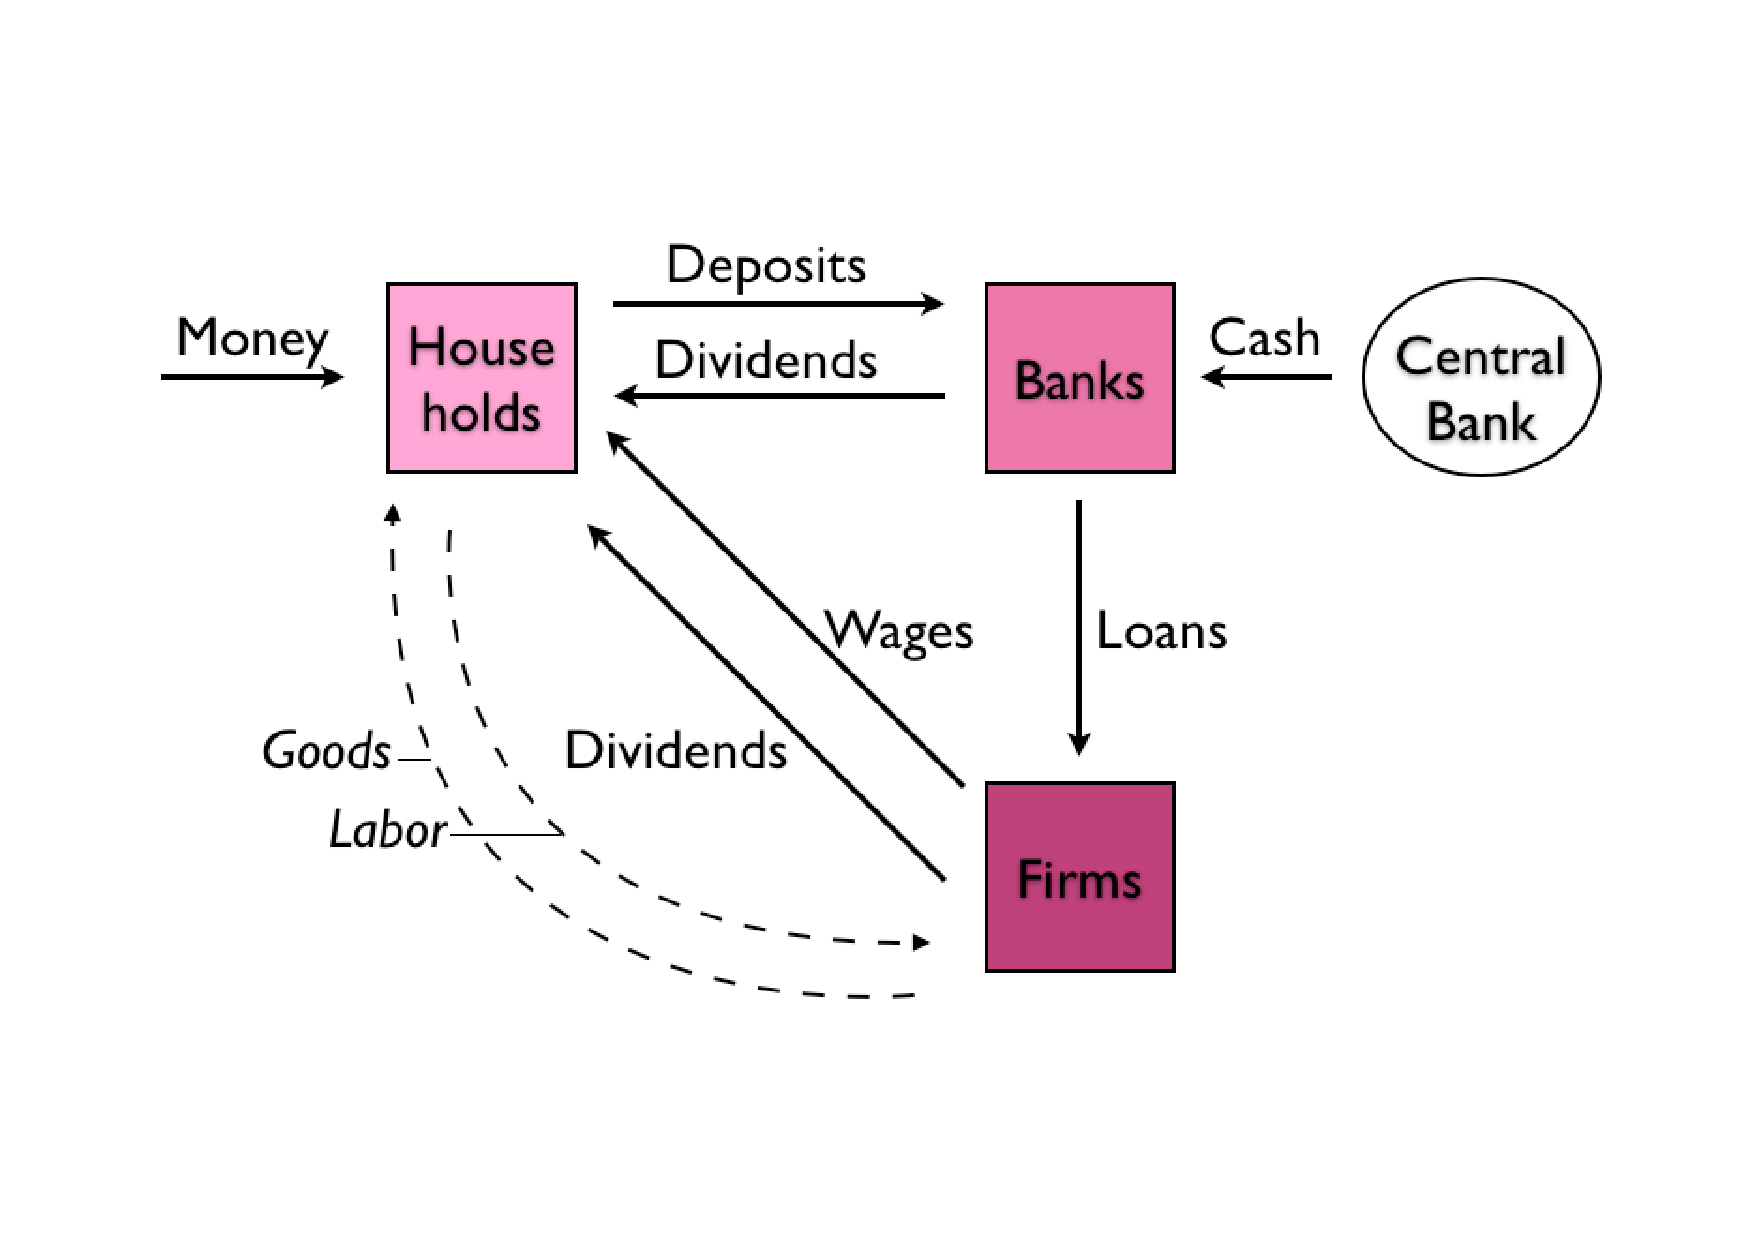
\includegraphics[width=1.0\textwidth]{P_SchorfMod} 
\end{center} 
\caption[CIA model illustration]{Continuous lines show the circulation of nominal funds, while dashed lines show the flow of real variables.} 
\end{figure}\\

The economy is made up of three central agents and one secondary agent: households, firms and banks (representing the financial sector), and a monetary authority which plays a minor role. Households maximize their utility function which depends on consumption, $C_t$, and hours worked, $H_t$, while deciding how much money to hold next period in cash, $M_{t+1}$ and how much to deposit at the bank, $D_t$, in order to earn $R_{H,t}-1$ interest. Households therefore solve the problem
\begin{eqnarray*}
\substack{\max \\ \{C_t,H_t,M_{t+1},D_t\}} & \mathbb{E}_0 \left[ \sum_{t=0}^\infty \beta^t \left[ (1-\phi) \ln C_t + \phi \ln (1-H_t) \right] \right] \\
\textrm{s.t.} & P_t C_t \leq M_t - D_t + W_t H_t \\
& 0 \leq D_t \\
& M_{t+1} = (M_t - D_t + W_tH_t - P_tC_t) + R_{H,t}D_t + F_t + B_t
\end{eqnarray*}
where the second equation spells out the cash in advance constraint including wage revenues, the third the inability to borrow from the bank and the fourth the intertemporal budget constraint emphasizing that households accumulate the money that remains after bank deposits and purchases on goods are deducted from total inflows made up of the money they receive from last period's cash balances, wages, interests, as well as dividends from firms, $F_t$, and from banks, $B_t$, which in both cases are made up of net cash inflows defined below. \\

Banks, on their end, receive cash deposits from households and a cash injection, $X_t$ from the central bank (which equals the net change in nominal money balances, $M_{t+1}-M_t$). It uses these funds to disburse loans to firms, $L_t$, on which they make a net return of $R_{F,t}-1$. Of course, banks are constrained in their loans by a credit market equilibrium condition $L_t \leq X_t + D_t$. Finally, bank dividends, $B_t$ are simply equal to $D_t + R_{F,t}L_t - R_{H,t}D_t - L_t + X_t$. \\

Finally, firms maximize the net present value of future dividends (discounted by the marginal utility of consumption, since they are owned by households) by choosing dividends, next period's capital stock, $K_{t+1}$, labor demand, $N_t$, and loans. Its problem is summarized by
\begin{eqnarray*}
\substack{\max \\ \{F_t,K_{t+1},N_{t},L_t\}} & \mathbb{E}_0 \left[ \sum_{t=0}^\infty \beta^{t+1} \frac{F_t}{C_{t+1}P_{t+1}} \right] \\
\textrm{s.t.} & F_t \leq L_t + P_t \left[ K_t^\alpha (A_t N_t)^{1-\alpha} - K_{t+1} + (1-\delta)K_t \right] - W_tN_t-L_tR_{F,t} \\
& W_tN_t \leq L_t\\
\end{eqnarray*}
where the second equation makes use of the production function \mbox{$Y_t = K_t^\alpha (A_t N_t)^{1-\alpha}$} and the real aggregate accounting constraint (goods market equilibrium) \mbox{$C_t + I_t = Y_t$}, where $I_t=K_{t+1} - (1-\delta)K_t$, and where $\delta$ is the rate of depreciation. Note that it is the firms that engage in investment in this model, by trading off investment for dividends to consumers. The third equation simply specifies that bank loans are used to pay for wage costs. \\

To close the model, we add the usual labor and money market equilibrium equations, $H_t= N_t$ and $P_tC_t=M_t + X_t$, as well as the condition that $R_{H,t}=R_{F,t}$ due to the equal risk profiles of the loans.\\

More importantly, we add a stochastic elements to the model. The model allows for two sources of perturbations, one real, affecting technology and one nominal, affecting the money stock. These important equations are
\[
\ln A_t = \gamma + \ln A_{t-1} + \epsilon_{A,t}, \qquad \epsilon_{A,t} \thicksim N(0,\sigma_A^2)
\]
and

\[
\ln m_t = (1-\rho)\ln m^* + \rho \ln m_{t-1} + \epsilon_{M,t}, \qquad \epsilon_{M,t} \thicksim N(0,\sigma_M^2)
\]
where $m_t \equiv M_{T+1}/M_t$ is the growth rate of the money stock. Note that theses expressions for trends are not written in the most straightforward manner nor very consistently. But we reproduced them never-the-less to make it easier to compare this example to the original paper. \\

The first equation is therefore a unit root with drift in the log of technology, and the second an autoregressive stationary process in the growth rate of money, but an AR(2) with a unit root in the log of the level of money. This can be seen from the definition of $m_t$ which can be rewritten as $\ln M_{t+1} = \ln M_t + \ln m_t$.\footnote{Alternatively, we could have written the AR(2) process in state space form and realized that the system has an eigenvalue of one. Otherwise said, one is a root of the second order autoregressive lag polynomial. As usual, if the logs of a variable are specified to follow a unit root process, the rate of growth of the series is a stationary stochastic process; see \citet{Hamilton1994}, chapter 15, for details.}\\

When the above functions are maximized, we obtain the following set of first order and equilibrium conditions. We will not dwell on the derivations here, to save space, but encourage you to browse \citet{CogleyNason1994} for additional details. We nonetheless give a brief intuitive explanation of each equation. The system comes down to
\begin{eqnarray*}
\mathbb{E}_{t}\bigg\{-\widehat{P}_{t}/\left[ \widehat{C}_{t+1}\widehat{P}_{t+1}m_{t}%
\right]\bigg\}&=&\beta e^{-\alpha (\gamma +\epsilon_{A,t+1})}P_{t+1}\Big[\alpha\widehat{K}_{t}^{\alpha -1}N_{t+1}^{1-\alpha }+
(1-\delta )\Big]\\
&&/\left[ 
\widehat{c}_{t+2}\widehat{P}_{t+2}m_{t+1}\right] \bigg\}\\
\widehat{W}_{t}&=&\widehat{L}_{t}/N_{t}\\
\frac{\phi }{1-\phi }\left[ \widehat{C}_{t}\widehat{P}_{t}/\left(
1-N_{t}\right) \right]&=&\widehat{L}_{t}/N_{t}\\
R_{t}&=&(1-\alpha )\widehat{P}_{t}e^{-\alpha (\gamma +\epsilon_{A,t+1})}\widehat{K}_{t-1}^{\alpha}N_{t}^{-\alpha }/\widehat{W}_{t}\\
\left[ \widehat{C}_{t}\widehat{P}_{t}\right] ^{-1}&=&\beta \left[ \left(
1-\alpha \right) \widehat{P}_{t}e^{-\alpha (\gamma +\epsilon_{A,t+1})}\widehat{K}_{t-1}^{\alpha}N_{t}^{1-\alpha }
\right]\\
&& \times  \mathbb{E}_{t}\left[\widehat{L}_{t}m_{t}\widehat{C}_{t+1}\widehat{P}_{t+1}\right] ^{-1}\\
\widehat{C}_t+\widehat{K}_t &=& e^{-\alpha(\gamma+\epsilon_{A,t})}\widehat{K}_{t-1}^\alpha N^{1-\alpha}+(1-\delta)e^{-(\gamma+\epsilon_{A,t})}\widehat{K}_{t-1}\\
\widehat{P}_t\widehat{C} &=& m_t\\
m_t-1+\widehat{D}_t &=& \widehat{L}_t\\
\widehat{Y}_t &=& \widehat{K}_{t-1}^\alpha N^{1-\alpha}e^{-\alpha (\gamma+\epsilon_{A,t})}\\
\ln(m_t) &=& (1-\rho)\ln(m^\star) + \rho\ln(m_{t-1})+\epsilon_{M,t}\\
\frac{A_t}{A_{t-1}}  \equiv  dA_t & = & \exp( \gamma + \epsilon_{A,t})\\
Y_t/Y_{t-1} &=& e^{\gamma+\epsilon_{A,t}}\widehat{Y}_t/\widehat{Y}_{t-1}\\
P_t/P_{t-1} &=& (\widehat{P}_t/\widehat{P}_{t-1})(m_{t-1}/e^{\gamma+\epsilon_{A,t}})
\end{eqnarray*}
where, importantly, hats over variables no longer mean deviations from steady state, but instead represent variables that have been made stationary. We come back to this important topic in details in section \ref{sec:nonstat} below. For now, we pause a moment to give some intuition for the above equations. In order, these equations correspond to:
\begin{enumerate}
\item The Euler equation in the goods market, representing the tradeoff to the economy of moving consumption goods across time.
\item The firms' borrowing constraint, also affecting labor demand, as firms use borrowed funds to pay for labor input.
\item The intertemporal labor market optimality condition, linking labor supply, labor demand, and the marginal rate of substitution between consumption and leisure. 
\item The equilibrium interest rate in which the marginal revenue product of labor equals the cost of borrowing to pay for that additional unit of labor.
\item The Euler equation in the credit market, which ensures that giving up one unit of consumption today for additional savings equals the net present value of future consumption.
\item The aggregate resource constraint.
\item The money market equilibrium condition equating nominal consumption demand to money demand to money supply to current nominal balances plus money injection. 
\item The credit market equilibrium condition.
\item The production function.
\item The stochastic process for money growth.
\item The stochastic process for technology.
\item The relationship between observable variables and stationary variables; more details on these last two equations appear in the following section. 
\end{enumerate}

\subsection{Declaring variables and parameters}
This block of the .mod file follows the usual conventions and would look like:\\
\\
\texttt{var m P c e W R k d n l Y\_obs P\_obs y dA; \\
varexo e\_a e\_m;\\
\\
parameters alp, bet, gam, mst, rho, psi, del;}\\
\\
where the choice of upper and lower case letters is not significant, the first set of endogenous variables, up to $l$, are as specified in the model setup above, and where the last five variables are defined and explained in more details in the section below on declaring the model in Dynare. The exogenous variables are as expected and concern the shocks to the evolution of technology and money balances. \\

\subsection{The origin of non-stationarity} \label{sec:nonstat}
The problem of non-stationarity comes from having stochastic trends in technology and money. The non-stationarity comes out clearly when attempting to solve the model for a steady state and realizing it does not have one. It can be shown that when shocks are null, real variables grow with $A_t$ (except for labor, $N_t$, which is stationary as there is no population growth), nominal variables grow with $M_t$ and prices with $M_t/A_t$. \textbf{Detrending} therefore involves the following operations (where hats over variables represent stationary variables): for real variables, $\hat q_t=q_t/A_t$, where $q_t = [y_t, c_t, i_t, k_{t+1} ]$. For nominal variables, $\hat{Q}_t = Q_t/M_t$, where $Q_t = [ d_t, l_t, W_t ]$. And for prices, $\hat P_t = P_t \cdot A_t / M_t$. \\

\subsection{Stationarizing variables}
Let's illustrate this transformation on output, and leave the transformations of the remaining equations as an exercise, if you wish (\citet{CogleyNason1994} includes more details on the transformations of each equation). We stationarize output by dividing its real variables (except for labor) by $A_t$. We define $\widehat{Y}_t$ to equal $Y_t / A_t$ and $\widehat{K}_t$ as $K_t / A_t$. \textsf{\textbf{NOTE!}} Recall from section \ref{sec:modspe} in chapter \ref{ch:solbase}), that in Dynare variables take the time subscript of the period in which they are decided (in the case of the capital stock, today's capital stock is a result of yesterday's decision). Thus, in the output equation, we should actually work with $\widehat{K}_{t-1}=K_{t-1} / A_{t-1}$. The resulting equation made up of stationary variables is
\begin{eqnarray*}
\frac{Y_t}{A_t} & = & \left( \frac{K_{t-1}}{A_{t-1}} \right)^\alpha A_t^{1-\alpha} N_t^{1-\alpha} A_t^{-1} A_{t-1}^\alpha \\
\widehat{Y}_t & = & \widehat{K}_{t-1}^\alpha N_t^{1-\alpha} \left( \frac{A_t}{A_{t-1}} \right)^{-\alpha} \\
& = & \widehat{K}_{t-1}^\alpha N_t^{1-\alpha} \exp(-\alpha (\gamma + \epsilon_{A,t}))
\end{eqnarray*}
where we go from the second to the third line by taking the exponential of both sides of the equation of motion of technology.\\

The above is the equation we retain for the .mod file of Dynare into which we enter:\\
\\
\texttt{y=k(-1)\textasciicircum alp*n\textasciicircum (1-alp)*exp(-alp*(gam+e\_a))}\\
\\

The other equations are entered into the .mod file after transforming them in exactly the same way as the one above. A final transformation to consider, that turns out to be useful since we often deal with the growth rate of technology, is to define \\
\\
\texttt{dA = exp(gam+e\_a)}\\
\\
by simply taking the exponential of both sides of the stochastic process of technology defined in the model setup above. \\

\subsection{Linking stationary variables to the data}
And finally, we must make a decision as to our \textbf{non-stationary observations}. We could simply stationarize them by \textbf{working with rates of growth} (which we know are constant). In the case of output, the observable variable would become $Y_t /Y_{t-1}$. We would then have to relate this observable, call it $gy\_{obs}$, to our (stationary) model's variables $\widehat Y_t$ by using the definition that $ \widehat{Y}_t \equiv Y_t/ A_t$. Thus, we add to the model block of the .mod file: \\
\\
\texttt{gy\_obs = dA*y/y(-1);}\\
\\
where, the $y$ of the .mod file are the stationary $\widehat Y_t$.\\

But, we could also \textbf{work with non-stationary data in levels}. This complicates things somewhat, but illustrates several features of Dynare worth highlighting; we therefore follow this path in the remainder of the example. The result is not very different, though, from what we just saw above. The goal is to add a line to the model block of our .mod file that relates the non stationary observables, call them $Y_{obs}$, to our stationary output, $\widehat Y_t$. We could simply write $Y_{obs} = \widehat Y_t A_t$. But since we don't have an $A_t$ variable, but just a $dA_t$, we we-write the above relationship in ratios. To the .mod file, we therefore add:\\
\\
\texttt{Y\_obs/Y\_obs(-1) = dA*y/y(-1);}\\
\\
We of course do the same for prices, our other observable variable, except that we use the relationship $P_{obs} = \widehat P_t M_t/A_t$ as noted earlier. The details of the correct transformations for prices are left as an exercise and can be checked against the results below.\\

\subsection{The resulting model block of the .mod file}

\texttt{model;\\
dA = exp(gam+e\_a);\\
log(m) = (1-rho)*log(mst) + rho*log(m(-1))+e\_m;\\
-P/(c(+1)*P(+1)*m)+bet*P(+1)*(alp*exp(-alp*(gam+log(e(+1))))*k\textasciicircum (alp-1)\\
*n(+1)\textasciicircum (1-alp)+(1-del)*exp(-(gam+log(e(+1)))))/(c(+2)*P(+2)*m(+1))=0;\\
W = l/n;\\
-(psi/(1-psi))*(c*P/(1-n))+l/n = 0;\\
R = P*(1-alp)*exp(-alp*(gam+e\_a))*k(-1)\textasciicircum alp*n\textasciicircum (-alp)/W;\\
1/(c*P)-bet*P*(1-alp)*exp(-alp*(gam+e\_a))*k(-1)\textasciicircum alp*n\textasciicircum (1-alp)/\\
(m*l*c(+1)*P(+1)) = 0;\\
c+k = exp(-alp*(gam+e\_a))*k(-1)\textasciicircum alp*n\textasciicircum (1-alp)+(1-del)\\
*exp(-(gam+e\_a))*k(-1);\\
P*c = m;\\
m-1+d = l;\\
e = exp(e\_a);\\
y = k(-1)\textasciicircum alp*n\textasciicircum (1-alp)*exp(-alp*(gam+e\_a));\\
Y\_obs/Y\_obs(-1) = dA*y/y(-1);\\
P\_obs/P\_obs(-1) = (p/p(-1))*m(-1)/dA;\\
end;}\\
\\
where, of course, the input conventions, such as ending lines with semicolons and indicating the timing of variables in parentheses, are the same as those listed in chapter \ref{ch:solbase}. \\

\textsf{\textbf{TIP!}} In the above model block, notice that what we have done is in fact relegated the non-stationarity of the model to just the last two equations, concerning the observables which are, after all, non-stationary. The problem that arises, though, is that we cannot linearize the above system in levels, as the last two equations don't have a steady state. If we first take logs, though, they become linear and it doesn't matter anymore where we calculate their derivative when taking a Taylor expansion of all the equations in the system. Thus, \textbf{when dealing with non-stationary observations, you must log-linearize your model} (and not just linearize it); this is a point to which we will return later. 

\subsection{Declaring observable variables}
We begin by declaring which of our model's variables are observables. In our .mod file we write\\
\\
\texttt{varobs P\_obs Y\_obs;}\\
\\
to specify that our observable variables are indeed $P\_obs$ and $Y\_obs$ as noted in the section above. \textsf{\textbf{NOTE!}} Recall from earlier that the number of observed variables must be smaller or equal to the number of shocks such that the model be estimated. If this is not the case, you should add measurement shocks to your model where you deem most appropriate. \\

\subsection{Declaring trends in observable variables}

Recall that we decided to work with the non-stationary observable variables in levels. Both output and prices exhibit stochastic trends. This can be seen explicitly by taking the difference of logs of output and prices to compute growth rates. In the case of output, we make use of the usual (by now!) relationship $Y_t=\widehat Y_t \cdot A_t$. Taking logs of both sides and subtracting the same equation scrolled back one period, we find:
\[
\Delta \ln Y_t = \Delta \ln \widehat Y_t + \gamma + \epsilon_{A,t}
\]
emphasizing clearly the drift term $\gamma$, whereas we know $\Delta \ln \widehat Y_t$ is stationary in steady state. \\

In the case of prices, we apply the same manipulations to show that:
\[
\Delta \ln P_t = \Delta \ln \widehat P_t + \ln m_{t-1} - \gamma - \epsilon_{A,t}
\]

Note from the original equation of motion of $\ln m_t$ that in steady state, $\ln m_t=\ln m^*$, so that the drift terms in the above equation are $\ln m^* - \gamma$.\footnote{This can also be see from substituting for $\ln m_{t-1}$ in the above equation with the equation of motion of $\ln m_t$ to yield: $\Delta \ln P_t = \Delta \ln \widehat P_t + \ln m^* + \rho(\ln m_{t-2}-\ln m^*) + \epsilon_{M,t} - \gamma - \epsilon_{A,t}$ where all terms on the right hand side are constant, except for $\ln m^*$ and $\gamma$.} \\

In Dynare, any trends, whether deterministic or stochastic (the drift term) must be declared up front. In the case of our example, we therefore write (in a somewhat cumbersome manner)\\
\\
\texttt{observation\_trends;\\
P\_obs (log(mst)-gam);\\
Y\_obs (gam);\\
end;}\\

In general, the command \texttt{observation\_trends} specifies linear trends as a function of model parameters for the observed variables in the model.\\

\subsection{Declaring unit roots in observable variables}

And finally, since P\_obs and Y\_obs inherit the unit root characteristics of their driving variables, technology and money, we must tell Dynare to use a diffuse prior (infinite variance) for their initialization in the Kalman filter. Note that for stationary variables, the unconditional covariance matrix of these variables is used for initialization. The algorithm to compute a true diffuse prior is taken from \citet{DurbinKoopman2001}. To give these instructions to Dynare, we write in the .mod\\
\\
\texttt{unit\_root\_vars P\_obs Y\_obs;}\\
\\
\textsf{\textbf{NOTE!}} You don't need to declare unit roots for any non-stationary model. Unit roots are only related to stochastic trends. You don't need to use a diffuse initial condition in the case of a deterministic trend, since the variance is finite.\\

\subsection{Specifying the steady state}
Declaring the steady state is just as explained in details and according to the same syntax explained in chapter \ref{ch:solbase}, covering the \texttt{initval}, \texttt{steady} and \texttt{check} commands. In chapter \ref{ch:estbase}, section \ref{sec:ssest}, we also discussed the usefulness of providing an external Matlab file to solve for the steady state. In this case, you can find the corresponding steady state file in the \textsl{models} folder under \textsl{UserGuide}. The file is called \textsl{fs2000ns\_steadystate.m}. There are some things to notice. First, the output of the function is the endogenous variables at steady state, the \texttt{ys} vector. The \texttt{check=0} limits steady state values to real numbers. Second, notice the declaration of parameters at the beginning; intuitive, but tedious... This functionality may be updated in later versions of Dynare. Third, note that the file is really only a sequential set of equalities, defining each variable in terms of parameters or variables solved in the lines above. So far, nothing has changed with respect to the equivalent file of chapter \ref{ch:estbase}. The only novelty is the declaration of the non-stationary variables, $P\_obs$ and $Y\_obs$ which take the value of 1. This is Dynare convention and must be the case for all your non-stationary variables. 

\subsection{Declaring priors}
We expand our .mod file with the following information: \\
\\
\texttt{estimated\_params;\\
alp, beta\_pdf, 0.356, 0.02; \\ 
bet, beta\_pdf, 0.993, 0.002; \\
gam, normal\_pdf, 0.0085, 0.003; \\
mst, normal\_pdf, 1.0002, 0.007; \\
rho, beta\_pdf, 0.129, 0.223;\\
psi, beta\_pdf, 0.65, 0.05;\\
del, beta\_pdf, 0.01, 0.005;\\
stderr e\_a, inv\_gamma\_pdf, 0.035449, inf;\\
stderr e\_m, inv\_gamma\_pdf, 0.008862, inf;\\
end;}\\
\\

\subsection{Launching the estimation}
We add the following commands to ask Dynare to run a basic estimation of our model:\\
\\
\texttt{estimation(datafile=fsdat,nobs=192,loglinear,mh\_replic=2000,\\
mode\_compute=4,mh\_nblocks=2,mh\_drop=0.45,mh\_jscale=0.65);}\\

\textsf{\textbf{NOTE!}} As mentioned earlier, we need to instruct Dynare to log-linearize our model, since it contains non-linear equations in non-stationary variables. A simple linearization would fail as these variables do not have a steady state. Fortunately, taking the log of the equations involving non-stationary variables does the job of linearizing them.\\

\subsection{The complete .mod file}
We have seen each part of the .mod separately; it's now time to get a picture of what the complete file looks like. For convenience, the file also appears in the \textsl{models} folder under \textsl{UserGuide} in your Dynare installation. The file is called \texttt{fs2000ns.mod}. \\
\\
\texttt{var m P c e W R k d n l Y\_obs P\_obs y dA; \\
varexo e\_a e\_m;\\
\\
parameters alp, bet, gam, mst, rho, psi, del;
\\
model;\\
dA = exp(gam+e\_a);\\
log(m) = (1-rho)*log(mst) + rho*log(m(-1))+e\_m;\\
-P/(c(+1)*P(+1)*m)+bet*P(+1)*(alp*exp(-alp*(gam+log(e(+1))))*k\textasciicircum (alp-1)\\
*n(+1)\textasciicircum (1-alp)+(1-del)*exp(-(gam+log(e(+1)))))/(c(+2)*P(+2)*m(+1))=0;\\
W = l/n;\\
-(psi/(1-psi))*(c*P/(1-n))+l/n = 0;\\
R = P*(1-alp)*exp(-alp*(gam+e\_a))*k(-1)\textasciicircum alp*n\textasciicircum (-alp)/W;\\
1/(c*P)-bet*P*(1-alp)*exp(-alp*(gam+e\_a))*k(-1)\textasciicircum alp*n\textasciicircum (1-alp)/(m*l*c(+1)*P(+1)) = 0;\\
c+k = exp(-alp*(gam+e\_a))*k(-1)\textasciicircum alp*n\textasciicircum (1-alp)+(1-del)*exp(-(gam+e\_a))*k(-1);\\
P*c = m;\\
m-1+d = l;\\
e = exp(e\_a);\\
y = k(-1)\textasciicircum alp*n\textasciicircum (1-alp)*exp(-alp*(gam+e\_a));\\
Y\_obs/Y\_obs(-1) = dA*y/y(-1);\\
P\_obs/P\_obs(-1) = (p/p(-1))*m(-1)/dA;\\
end;\\
\\
varobs P\_obs Y\_obs;\\
\\
observation\_trends;\\
P\_obs (log(mst)-gam);\\
Y\_obs (gam);\\
end;\\
\\
unit\_root\_vars = P\_obs Y\_obs;\\
\\
initval;\\
k = 6;\\
m = mst;\\
P = 2.25;\\
c = 0.45;\\
e = 1;\\
W = 4;\\
R = 1.02;\\
d = 0.85;\\
n = 0.19;\\
l = 0.86;\\
y = 0.6;\\
dA = exp(gam);\\
end;\\
\\
// the above is really only useful if you want to do a stoch\_simul\\
// of your model, since the estimation will use the Matlab\\
// steady state file also provided and discussed above.\\
\\
steady;\\
\\
estimated\_params;\\
alp, beta\_pdf, 0.356, 0.02; \\ 
bet, beta\_pdf, 0.993, 0.002; \\
gam, normal\_pdf, 0.0085, 0.003; \\
mst, normal\_pdf, 1.0002, 0.007; \\
rho, beta\_pdf, 0.129, 0.223;\\
psi, beta\_pdf, 0.65, 0.05;\\
del, beta\_pdf, 0.01, 0.005;\\
stderr e\_a, inv\_gamma\_pdf, 0.035449, inf;\\
stderr e\_m, inv\_gamma\_pdf, 0.008862, inf;\\
end;\\
\\
estimation(datafile=fsdat,nobs=192,loglinear,mh\_replic=2000,\\
mode\_compute=4,mh\_nblocks=2,mh\_drop=0.45,mh\_jscale=0.65);}\\
\\

\subsection{Summing it up}
The explanations given above of each step necessary to translate the \citet{Schorfheide2000} example into language that Dynare can understand and process was quite lengthy and involved a slew of new commands and information. It may therefore be useful, to gain a ``bird's eyeview'' on what we have just accomplished, and summarize the most important steps at a high level. This is done in figure \ref{fig:estsumm}.\\
\begin{figure} \label{fig:estsumm}
\begin{center} 
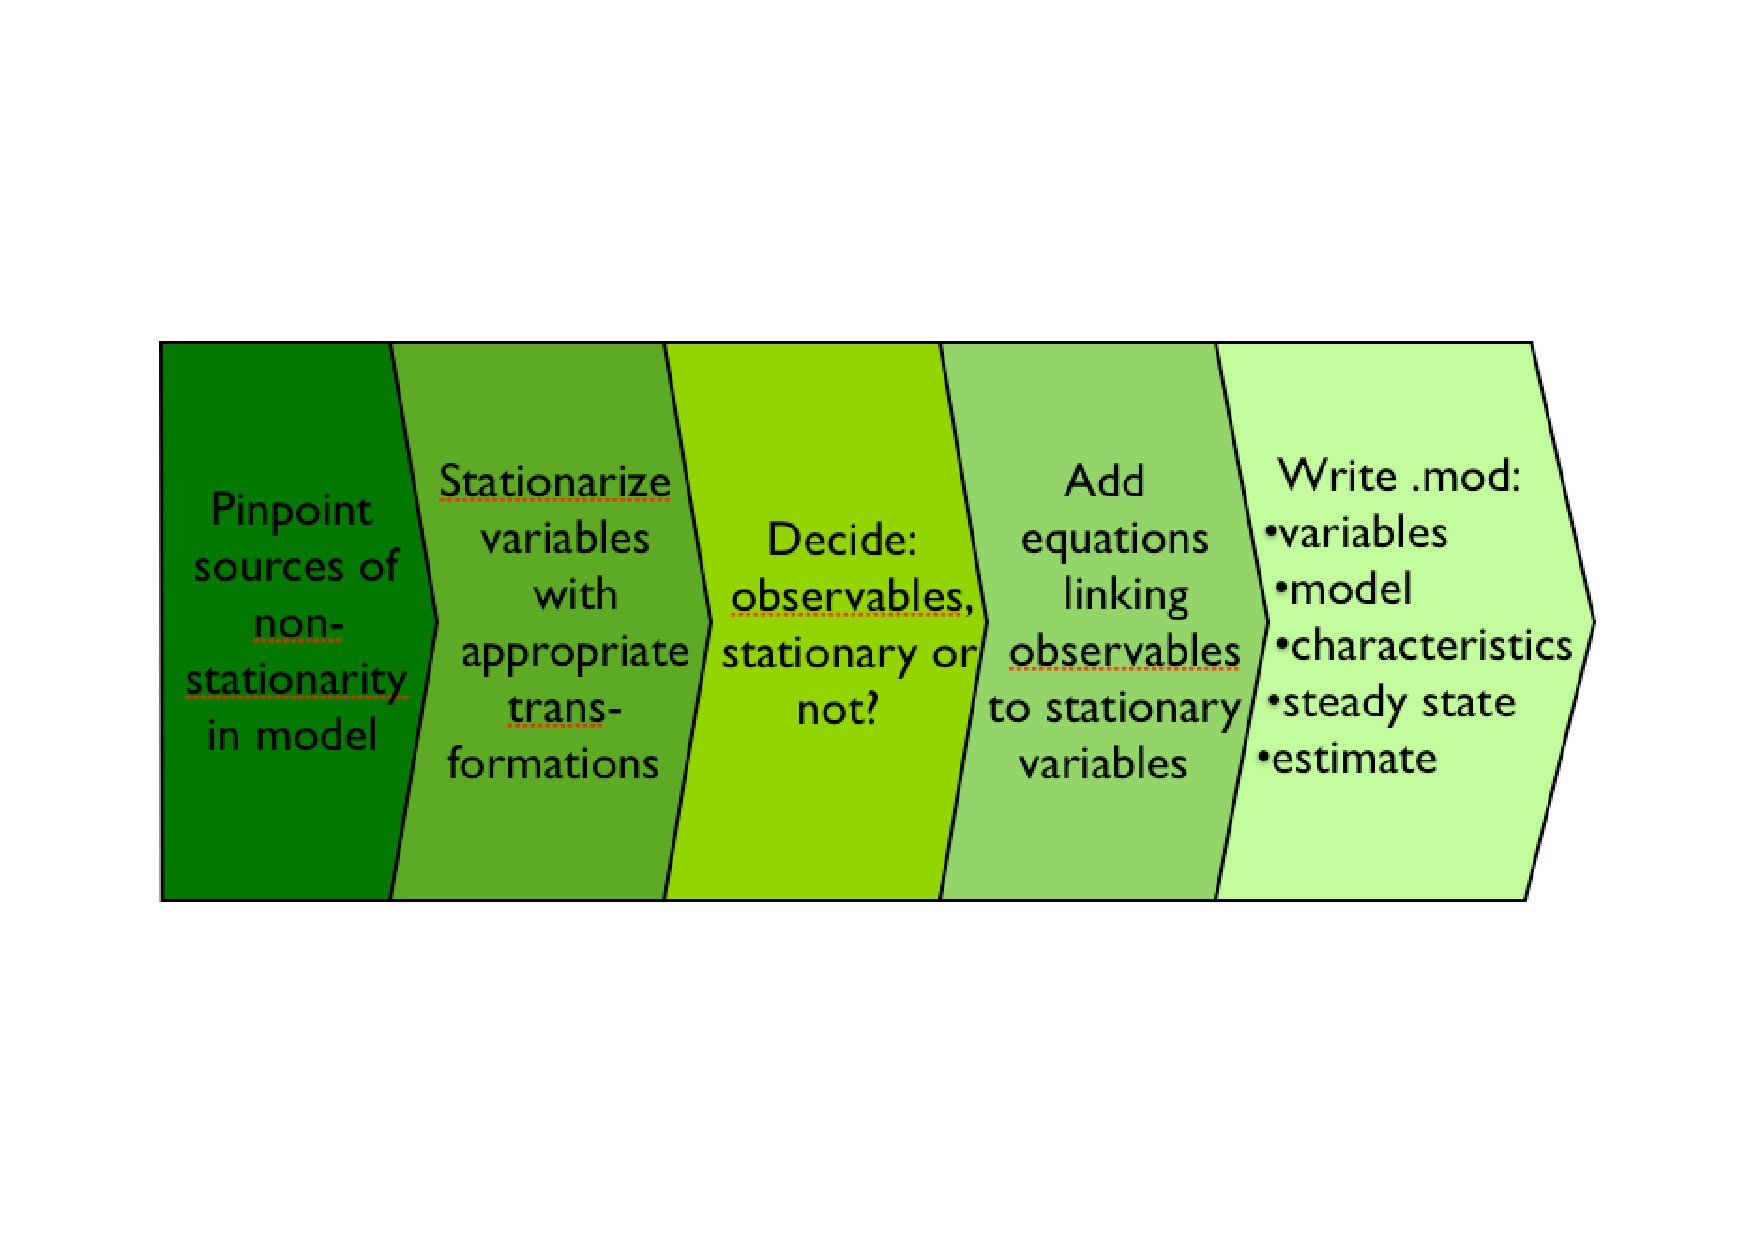
\includegraphics[width=1.0\textwidth]{P_flowest} 
\end{center} 
\caption[Steps of model estimation]{At a high level, there are five basic steps to translate a model into Dynare for successful estimation.} 
\end{figure}\\


\section{Comparing models based on their posterior distributions}
** TBD

\section{Where is your output stored?}
The output from estimation can be extremely varied, depending on the instructions you give Dynare. The \href{http://www.dynare.org/documentation-and-support/manual}{Reference Manual} overviews the complete set of potential output files and describes where you can find each one. 
\chapter{Solving DSGE models - Behind the scenes of Dynare} \label{ch:solbeh}

\section{Introduction}
The aim of this chapter is to peer behind the scenes of Dynare, or under its hood, to get an idea of the methodologies and algorithms used in its computations. Going into details would be beyond the scope of this User Guide which will instead remain at a high level. What you will find below will either comfort you in realizing that Dynare does what you expected of it - and what you would have also done if you had had to code it all yourself (with a little extra time on your hands!), or will spur your curiosity to have a look at more detailed material. If so, you may want to go through Michel Juillard's presentation on solving DSGE models to a first and second order (available on Michel Juillard's \href{http://jourdan.ens.fr/~michel/}{website}), or read \citet{CollardJuillard2001b} or \citet{SchmittGrohe2004} which gives a good overview of the most recent solution techniques based on perturbation methods. Finally, note that in this chapter we will focus on stochastic models - which is where the major complication lies, as explained in section \ref{sec:detstoch} of chapter \ref{ch:solbase}. For more details on the Newton-Raphson algorithm used in Dynare to solve deterministic models, see \citet{Juillard1996}. \\

\section{What is the advantage of a second order approximation?}
As noted in chapter \ref{ch:solbase} and as will become clear in the section below, linearizing a system of equations to the first order raises the issue of certainty equivalence. This is because only the first moments of the shocks enter the linearized equations, and when expectations are taken, they disappear. Thus, unconditional expectations of the endogenous variables are equal to their non-stochastic steady state values. \\

This may be an acceptable simplification to make. But depending on the context, it may instead be quite misleading. For instance, when using second order welfare functions to compare policies, you also need second order approximations of the policy function. Yet more clearly, in the case of asset pricing models, linearizing to the second order enables you to take risk (or the variance of shocks) into consideration - a highly desirable modeling feature. It is therefore very convenient that Dynare allows you to choose between a first or second order linearization of your model in the option of the \texttt{stoch\_simul} command. \\

\section{How does dynare solve stochastic DSGE models?}
In this section, we shall briefly overview the perturbation methods employed by Dynare to solve DSGE models to a first order approximation. The second order follows very much the same approach, although at a higher level of complexity. The summary below is taken mainly from Michel Juillard's presentation ``Computing first order approximations of DSGE models with Dynare'', which you should read if interested in particular details, especially regarding second order approximations (available on Michel Juillard's \href{http://jourdan.ens.fr/~michel/}{website}). \\

To summarize, a DSGE model is a collection of first order and equilibrium conditions that take the general form: 
\[
\mathbb{E}_t\left\{f(y_{t+1},y_t,y_{t-1},u_t)\right\}=0
\]
\begin{eqnarray*}
\mathbb{E}(u_t) &=& 0\\
\mathbb{E}(u_t u_t') &=& \Sigma_u
\end{eqnarray*}
and where:
\begin{description}
  \item[$y$]: vector of endogenous variables of any dimension
  \item[$u$]: vector of exogenous stochastic shocks of any dimension
\end{description}

The solution to this system is a set of equations relating variables in the current period to the past state of the system and current shocks, that satisfy the original system. This is what we call the policy function. Sticking to the above notation, we can write this function as:
\[
y_t = g(y_{t-1},u_t)
\]

Then, it is straightforward to re-write $y_{t+1}$ as
\begin{eqnarray*}
  y_{t+1} &=& g(y_t,u_{t+1})\\
  &=& g(g(y_{t-1},u_t),u_{t+1})\\
\end{eqnarray*}

We can then define a new function $F$, such that:
\[
F(y_{t-1},u_t,u_{t+1}) =
f(g(g(y_{t-1},u_t),u_{t+1}),g(y_{t-1},u_t),y_{t-1},u_t)\\
\]
which enables us to rewrite our system in terms of past variables, and current and future shocks:
\[
\mathbb{E}_t\left[F(y_{t-1},u_t,u_{t+1})\right] = 0
\]

We then venture to linearize this model around a steady state defined as:
\[
f(\bar y, \bar y, \bar y, 0) = 0
\]
having the property that:
\[
\bar y = g(\bar y, 0)
\]

The first order Taylor expansion around $\bar y$ yields:
\begin{eqnarray*}
\lefteqn{\mathbb{E}_t\left\{F^{(1)}(y_{t-1},u_t,u_{t+1})\right\} =}\\
&& \mathbb{E}_t\Big[f(\bar y, \bar y, \bar y)+f_{y_+}\left(g_y\left(g_y\hat y+g_uu \right)+g_u u' \right)\\
&& + f_{y_0}\left(g_y\hat y+g_uu \right)+f_{y_-}\hat y+f_u u\Big]\\
&& = 0
\end{eqnarray*}
with $\hat y = y_{t-1} - \bar y$, $u=u_t$, $u'=u_{t+1}$, $f_{y_+}=\frac{\partial f}{\partial y_{t+1}}$, $f_{y_0}=\frac{\partial f}{\partial y_t}$, $f_{y_-}=\frac{\partial f}{\partial y_{t-1}}$, $f_{u}=\frac{\partial f}{\partial u_t}$, $g_y=\frac{\partial g}{\partial y_{t-1}}$, $g_u=\frac{\partial g}{\partial u_t}$.\\

Taking expectations (we're almost there!):
\begin{eqnarray*}
   \lefteqn{\mathbb{E}_t\left\{F^{(1)}(y_{t-1},u_t, u_{t+1})\right\} =}\\
&& f(\bar y, \bar y, \bar y)+f_{y_+}\left(g_y\left(g_y\hat y+g_uu \right) \right)\\
&& + f_{y_0}\left(g_y\hat y+g_uu \right)+f_{y_-}\hat y+f_u u\Big\}\\
&=& \left(f_{y_+}g_yg_y+f_{y_0}g_y+f_{y_-}\right)\hat y+\left(f_{y_+}g_yg_u+f_{y_0}g_u+f_{u}\right)u\\
&=& 0\\
\end{eqnarray*}

As you can see, since future shocks only enter with their first moments (which are zero in expectations), they drop out when taking expectations of the linearized equations. This is technically why certainty equivalence holds in a system linearized to its first order. The second thing to note is that we have two unknown variables in the above equation: $g_y$ and $g_u$ each of which will help us recover the policy function $g$. \\

Since the above equation holds for any $\hat y$ and any $u$, each parenthesis must be null and we can solve each at a time. The first, yields a quadratic equation  in $g_y$, which we can solve with a series of algebraic trics that are not all immediately apparent (but detailed in Michel Juillard's presentation). Incidentally, one of the conditions that comes out of the solution of this equation is the Blanchard-Kahn condition: there must be as many roots larger than one in modulus as there are forward-looking variables in the model. Having recovered $g_y$, recovering $g_u$ is then straightforward from the second parenthesis. \\

Finally, notice that a first order linearization of the function $g$ yields:
\[
y_t = \bar y+g_y\hat y+g_u u
\]
And now that we have $g_y$ and $g_u$, we have solved for the (approximate) policy (or decision) function and have succeeded in solving our DSGE model. If we were interested in impulse response functions, for instance, we would simply iterate the policy function starting from an initial value given by the steady state. \\

The second order solution uses the same ``perturbation methods'' as above (the notion of starting from a function you can solve - like a steady state - and iterating forward), yet applies more complex algebraic techniques to recover the various partial derivatives of the policy function. But the general approach is perfectly isomorphic. Note that in the case of a second order approximation of a DSGE model, the variance of future shocks remains after taking expectations of the linearized equations and therefore affects the level of the resulting policy function.\\

\chapter{Estimating DSGE models - Behind the scenes of Dynare} \label{ch:estbeh}

This chapter focuses on the theory of Bayesian estimation. It begins by motivating Bayesian estimation by suggesting some arguments in favor of it as opposed to other forms of model estimation. It then attempts to shed some light on what goes on in Dynare's machinery when it estimates DSGE models. To do so, this section surveys the methodologies adopted for Bayesian estimation, including defining what are prior and posterior distributions, using the Kalman filter to find the likelihood function, estimating the posterior function thanks to the Metropolis-Hastings algorithm, and comparing models based on posterior distributions.


\section{Advantages of Bayesian estimation}

Bayesian estimation is becoming increasingly popular in the field of macro-economics. Recent papers have attracted significant attention; some of these include:  \citet{Schorfheide2000} which uses Bayesian methods to compare the fit of two competing DSGE models of consumption, \citet{LubikSchorfheide2003} which investigates whether central banks in small open economies respond to exchange rate movements, \citet{SmetsWouters2003} which applies Bayesian estimation techniques to a model of the Eurozone, \citet{Ireland2004} which emphasizes instead maximum likelihood estimation, \citet{VillaverdeRubioRamirez2004} which reviews the econometric properties of Bayesian estimators and compare estimation results with maximum likelihood and BVAR methodologies, \citet{LubikSchorfheide2005} which applies Bayesian estimation methods to an open macro model focussing on issues of misspecification and identification, and finally \citet{RabanalRubioRamirez2005} which compares the fit, based on posterior distributions, of four competing specifications of New Keynesian monetary models with nominal rigidities.\\

There are a multitude of advantages of using Bayesian methods to estimate a model, but five of these stand out as particularly important and general enough to mention here.\\

First, Bayesian estimation fits the complete, solved DSGE model, as opposed to GMM estimation which is based on particular equilibrium relationships such as the Euler equation in consumption. Likewise, estimation in the Bayesian case is based on the likelihood generated by the DSGE system, rather than the more indirect discrepancy between the implied DSGE and VAR impulse response functions. Of course, if your model is entirely mis-specified, estimating it using Bayesian techniques could be a disadvantage.\\

Second, Bayesian techniques allow the consideration of priors which work as weights in the estimation process so that the posterior distribution avoids peaking at strange points where the likelihood peaks. Indeed, due to the stylized and often misspecified nature of DSGE models, the likelihood often peaks in regions of the parameter space that are contradictory with common observations, leading to the ``dilemma of absurd parameter estimates''.\\

Third, the inclusion of priors also helps identifying parameters. Unfortunately, when estimating a model, the problem of identification often arises. It can be summarized by different values of structural parameters leading to the same joint distribution for observables. More technically, the problem arises when the posterior distribution is flat over a subspace of parameter values. But the weighting of the likelihood with prior densities often leads to adding just enough curvature in the posterior distribution to facilitate numerical maximization.\\

Fourth, Bayesian estimation explicitly addresses model misspecification by including shocks, which can be interpreted as observation errors, in the structural equations.\\

Sixth, Bayesian estimation naturally leads to the comparison of models based on fit. Indeed, the posterior distribution corresponding to competing models can easily be used to determine which model best fits the data. This procedure, as other topics mentioned above, is discussed more technically in the subsection below. 


\section{The basic mechanics of Bayesian estimation}
This and the following subsections are based in great part on work by, and discussions with, St�phane Adjemian, a member of the Dynare development team. Some of this work, although summarized in presentation format, is available in the ``Events'' page of the \href{http://www.dynare.org/events/workshop-on-learning-and-monetary-policy}{Dynare website}. Other helpful material includes \citet{AnSchorfheide2006}, which includes a clear and quite complete introduction to Bayesian estimation, illustrated by the application of a simple DSGE model. Also, the appendix of \citet{Schorfheide2000} contains details as to the exact methodology and possible difficulties encountered in Bayesian estimation. You may also want to take a glance at \citet{Hamilton1994}, chapter 12, which provides a very clear, although somewhat outdated, introduction to the basic mechanics of Bayesian estimation. Finally, the websites of \href{http://www.econ.upenn.edu/~schorf/}{Frank Schorfheide} and \href{http://www.econ.upenn.edu/~jesusfv/index.html}{Jesus Fernandez-Villaverde} contain a wide variety of very helpful material, from example files to lecture notes to related papers. Finally, remember to also check the \href{http://www.dynare.org/documentation-and-support/examples}{open online examples} of the Dynare website for examples of .mod files touching on Bayesian estimation. \\

At its most basic level, Bayesian estimation is a bridge between calibration and maximum likelihood. The tradition of calibrating models is inherited through the specification of priors. And the maximum likelihood approach enters through the estimation process based on confronting the model with data. Together, priors can be seen as weights on the likelihood function in order to give more importance to certain areas of the parameter subspace. More technically, these two building blocks - priors and likelihood functions - are tied together by Bayes' rule. Let's see how. \\

First, priors are described by a density function of the form  
\[ p(\boldsymbol\theta_{\mathcal A}|\mathcal A) \] where $\mathcal A$ stands for a specific model, $\boldsymbol\theta_{\mathcal A}$ represents the parameters of model $\mathcal A$, $p(\bullet)$ stands for a probability density function (pdf) such as a normal, gamma, shifted gamma, inverse gamma, beta, generalized beta, or uniform function. \\

Second, the likelihood function describes the density of the observed
        data, given the model and its parameters:
        \[
            {\mathcal L}(\boldsymbol\theta_{\mathcal A}|\mathbf Y_T,\mathcal A) \equiv p(\mathbf Y_T | \boldsymbol\theta_{\mathcal A}, \mathcal A)
        \]
        where $\mathbf Y_T$ are the observations until period
        $T$, and where in our case the likelihood is recursive and can be written as:
        \[
            p(\mathbf Y_T | \boldsymbol\theta_{\mathcal A}, \mathcal A) =
            p(y_0|\boldsymbol\theta_{\mathcal A},\mathcal A)\prod^T_{t=1}p(y_t | \mathbf Y_{t-1},\boldsymbol\theta_{\mathcal A}, \mathcal A)
        \]

We now take a step back. Generally speaking, we have a prior density $p(\boldsymbol\theta)$ on the one hand, and on the other, a likelihood $p(\mathbf Y_T | \boldsymbol\theta)$. In the end, we are interested in $p(\boldsymbol\theta | \mathbf Y_T)$, the \textbf{posterior
        density}. Using the \textbf{Bayes theorem} twice we obtain this density of parameters
        knowing the data. Generally, we have
         \[p(\boldsymbol\theta | \mathbf Y_T) = \frac{p(\boldsymbol\theta ; \mathbf Y_T) }{p(\mathbf Y_T)}\]

We also know that
    \[
        p(\mathbf Y_T |\boldsymbol\theta ) = \frac{p(\boldsymbol\theta ; \mathbf Y_T)}{p(\boldsymbol\theta)}
        \Leftrightarrow p(\boldsymbol\theta ; \mathbf Y_T) = p(\mathbf Y_T |\boldsymbol\theta)\times
        p(\boldsymbol\theta)
    \]

By using these identities, we can combine the \textbf{prior density} and the \textbf{likelihood function} discussed above to get the posterior density:
        \[
            p(\boldsymbol\theta_{\mathcal A} | \mathbf Y_T, \mathcal A) = \frac{p(\mathbf Y_T |\boldsymbol\theta_{\mathcal A}, \mathcal A)p(\boldsymbol\theta_{\mathcal A}|\mathcal A)}{p(\mathbf Y_T|\mathcal A)}
        \]
where $p(\mathbf Y_T|\mathcal A)$ is the \textbf{marginal density} of the data
        conditional on the model:
        \[
            p(\mathbf Y_T|\mathcal A) = \int_{\Theta_{\mathcal A}} p(\boldsymbol\theta_{\mathcal A} ; \mathbf Y_T
            |\mathcal A) d\boldsymbol\theta_{\mathcal A}
        \]

Finally, the \textbf{posterior kernel} (or un-normalized posterior density, given that the marginal density above is a constant or equal for any parameter), corresponds to the numerator of the posterior density:
        \[
            p(\boldsymbol\theta_{\mathcal A} | \mathbf Y_T, \mathcal A) \propto p(\mathbf Y_T |\boldsymbol\theta_{\mathcal A},
            \mathcal A)p(\boldsymbol\theta_{\mathcal A}|\mathcal A) \equiv \mathcal K(\boldsymbol\theta_{\mathcal A} | \mathbf Y_T, \mathcal A)
        \]
This is the fundamental equation that will allow us to rebuild all posterior moments of interest. The trick will be to estimate the likelihood function with the help of the \textbf{Kalman filter} and then simulate the posterior kernel using a sampling-like or Monte Carlo method such as the \textbf{Metropolis-Hastings}. These topics are covered in more details below. Before moving on, though, the subsection below gives a simple example based on the above reasoning of what we mean when we say that Bayesian estimation is ``somewhere in between calibration and maximum likelihood estimation''. The example is drawn from \citet{Zellner1971}, although other similar examples can be found in \citet{Hamilton1994}, chapter 12.\\

\subsection{Bayesian estimation: somewhere between calibration and maximum likelihood estimation - an example}

Suppose a data generating process $y_t = \mu + \varepsilon_t$ for $t=1,...,T$, where $\varepsilon_t \sim \mathcal{N}(0,1)$ is gaussian white noise. Then, the likelihood is given by
            \[
                p(\mathbf{Y}_T|\mu) =
                (2\pi)^{-\frac{T}{2}}e^{-\frac{1}{2}\sum_{t=1}^T(y_t-\mu)^2}
            \]
We know from the above that $\widehat{\mu}_{ML,T} = \frac{1}{T}\sum_{t=1}^T y_t \equiv
                \overline{y}$ and that $\mathbb{V}[\widehat{\mu}_{ML,T}] = \frac{1}{T}$. \\
                
In addition, let our prior be a gaussian distribution with expectation
            $\mu_0$ and variance $\sigma_{\mu}^2$. Then, the posterior density is defined, up to a constant, by:
            \[
                p\left(\mu|\mathbf{Y}_T\right) \propto
                (2\pi\sigma_{\mu}^2)^{-\frac{1}{2}}e^{-\frac{1}{2}\frac{(\mu-\mu_0)^2}{\sigma_{\mu}^2}}\times(2\pi)^{-\frac{T}{2}}e^{-\frac{1}{2}\sum_{t=1}^T(y_t-\mu)^2}
            \]
Or equivalently, $p\left(\mu|\mathbf{Y}_T\right) \propto
                e^{-\frac{\left(\mu-\mathbb{E}[\mu]\right)^2}{\mathbb{V}[\mu]}}$, with
            \[
                \mathbb{V}[\mu] = \frac{1}{\left(\frac{1}{T}\right)^{-1} +
                \sigma_{\mu}^{-2}}
            \]
            and
            \[
                \mathbb{E}[\mu] =
                \frac{\left(\frac{1}{T}\right)^{-1}\widehat{\mu}_{ML,T} +
                \sigma_{\mu}^{-2}\mu_0}{\left(\frac{1}{T}\right)^{-1} +
                \sigma_{\mu}^{-2}}
            \]

From this, we can tell that the posterior mean is a convex combination of the prior mean and the ML estimate. In particular, if $\sigma_{\mu}^2 \rightarrow \infty$ (ie, we have no prior information, so we just estimate the model) then $\mathbb{E}[\mu] \rightarrow \widehat{\mu}_{ML,T}$, the maximum likelihood estimator. But if $\sigma_{\mu}^2 \rightarrow 0$ (ie, we're sure of ourselves and we calibrate the parameter of interest, thus leaving no room for estimation) then $\mathbb{E}[\mu] \rightarrow \mu_0$, the prior mean. Most of the time, we're somewhere in the middle of these two extremes. 


\section{DSGE models and Bayesian estimation}
\subsection{Rewriting the solution to the DSGE model}
Recall from chapter \ref{ch:solbeh} that any DSGE model, which is really a collection of first order and equilibrium conditions, can be written in the form $\mathbb{E}_t\left\{f(y_{t+1},y_t,y_{t-1},u_t)\right\}=0$, taking as a solution equations of the type $y_t = g(y_{t-1},u_t)$, which we call the decision rule. In more appropriate terms for what follows, we can rewrite the solution to a DSGE model as a system in the following manner:
  \begin{eqnarray*}
    y^*_t &=& M\bar y(\theta)+M\hat y_t+N(\theta)x_t+\eta_t\\
\hat y_t &=& g_y(\theta)\hat y_{t-1}+g_u(\theta)u_t\\
E(\eta_t \eta_t') &=& V(\theta)\\
E(u_t u_t') &=& Q(\theta)
  \end{eqnarray*}
where $\hat y_t$ are variables in deviations from steady state, $\bar y$ is the vector of steady state values and $\theta$ the vector of deep (or structural) parameters to be estimated. Other variables are described below.\\

The second equation is the familiar decision rule mentioned above. But the equation expresses a relationship among true endogenous variables that are not directly observed. Only $y^*_t$ is observable, and it is related to the true variables with an error $\eta_t$. Furthermore, it may have a trend, which is captured with $N(\theta)x_t$ to allow for the most general case in which the trend depends on the deep parameters. The first and second equations above therefore naturally make up a system of measurement and transition or state equations, respectively, as is typical for a Kalman filter (you guessed it, it's not a coincidence!). \\

\subsection{Estimating the likelihood function of the DSGE model}
The next logical step is to estimate the likelihood of the DSGE solution system mentioned above. The first apparent problem, though, is that the equations are non linear in the deep parameters. Yet, they are linear in the endogenous and exogenous variables so that the likelihood may be evaluated with a linear prediction error algorithm like the Kalman filter. This is exactly what Dynare does. As a reminder, here's what the Kalman filter recursion does.\\

For $t=1,\ldots,T$ and with initial values $y_1$ and $P_1$ given, the recursion follows
\begin{eqnarray*}
  v_t &=& y^*_t - \bar y^* - M\hat y_t - Nx_t\\
  F_t &=& M P_t M'+V\\
  K_t &=& g_yP_tg_y'F_t^{-1}\\
  \hat y_{t+1} &=& g_y \hat y_t+K_tv_t\\
  P_{t+1} &=& g_y P_t (g_y-K_tM)'+g_uQg_u'
\end{eqnarray*}
For more details on the Kalman filter, see \citet{Hamilton1994}, chapter 13. \\

From the Kalman filter recursion, it is possible to derive the \textbf{log-likelihood} given by
\[
\ln \mathcal{L}\left(\boldsymbol\theta|\mathbf Y^*_T\right) = -\frac{Tk}{2}\ln(2\pi)-\frac{1}{2}\sum_{t=1}^T|F_t|-\frac{1}{2}v_t'F_t^{-1}v_t  
\]
where the vector $\boldsymbol\theta$ contains the parameters we have to estimate: $\theta$, $V(\theta)$ and $Q(\theta)$ and where $Y^*_T$ expresses the set of observable endogenous variables $y^*_t$ found in the measurement equation. \\

The log-likelihood above gets us one step closer to our goal of finding the posterior distribution of our parameters. Indeed, the \textbf{log posterior kernel} can be expressed as 
\[
\ln \mathcal{K}(\boldsymbol\theta|\mathbf Y^*_T) = \ln \mathcal{L}\left(\boldsymbol\theta|\mathbf Y^*_T\right) + \ln p(\boldsymbol\theta)
\]
where the first term on the right hand side is now known after carrying out the Kalman filter recursion. The second, recall, are the priors, and are also known. \\

\subsection{Finding the mode of the posterior distribution}
Next, to find the mode of the posterior distribution - a key parameter and an important output of Dynare - we simply maximize the above log posterior kernel with respect to $\theta$. This is done in Dynare using numerical methods. Recall that the likelihood function is not Gaussian with respect to $\theta$ but to functions of $\theta$ as they appear in the state equation. Thus, this maximization problem is not completely straightforward, but fortunately doable with modern computers. \\

\subsection{Estimating the posterior distribution}
Finally, we are now in a position to find the posterior distribution of our parameters. The distribution will be given by the kernel equation above, but again, it is a nonlinear and complicated function of the deep parameters $\theta$. Thus, we cannot obtain an explicit form for it. We resort, instead, to sampling-like methods, of which the Metropolis-Hastings has been retained in the literature as particularly efficient. This is indeed the method adopted by Dynare.\\

The general idea of the Metropolis-Hastings algorithm is to simulate the posterior distribution. It is a ``rejection sampling algorithm'' used to generate a sequence of samples (also known as a ``Markov Chain'' for reasons that will become apparent later) from a distribution that is unknown at the outset. Remember that all we have is the posterior mode; we are instead more often interested in the mean and variance of the estimators of $\theta$. To do so, the algorithm builds on the fact that under general conditions the distribution of the deep parameters will be asymptotically normal. The algorithm, in the words of An and Shorfheide, ``constructs a Gaussian approximation around the posterior mode and uses a scaled version of the asymptotic covariance matrix as the covariance matrix for the proposal distribution. This allows for an efficient exploration of the posterior distribution at least in the neighborhood of the mode'' (\citet{AnSchorfheide2006}, p. 18). More precisely, the \textbf{Metropolis-Hastings algorithm implements the following steps}: 
\begin{enumerate}
        \item Choose a starting point $\boldsymbol\theta^\circ$, where this is typically the posterior mode, and run a loop over
        2-3-4. 
        \item Draw a \emph{proposal} $\boldsymbol\theta^*$ from a \emph{jumping} distribution
        \[
            J(\boldsymbol\theta^*|\boldsymbol\theta^{t-1}) =
            \mathcal N(\boldsymbol\theta^{t-1},c\Sigma_{m})
        \]
        where $\Sigma_{m}$ is the inverse of the Hessian computed at the posterior mode.
        \item Compute the acceptance ratio
        \[
            r = \frac{p(\boldsymbol\theta^*|\mathbf Y_T)}{p(\boldsymbol\theta^{t-1}|\mathbf
            Y_T)} = \frac{\mathcal K(\boldsymbol\theta^*|\mathbf Y_T)}{\mathcal K(\boldsymbol\theta^{t-1}|\mathbf
            Y_T)}
        \]
        \item Finally accept or discard the proposal $\boldsymbol\theta^*$  according to the following rule, and update, if necessary, the jumping distribution:
        \[
            \boldsymbol\theta^t = \left\{
            \begin{array}{ll}
                \boldsymbol\theta^* & \mbox{ with probability $\min(r,1)$}\\
                \boldsymbol\theta^{t-1} & \mbox{ otherwise.}
            \end{array}\right.
        \]
    \end{enumerate}

Figure \ref{fig:MH} tries to clarify the above. In step 1, choose a candidate paramter, $\theta^*$ from a Normal distribution, whose mean has been set to $\theta^{t-1}$ (this will become clear in just a moment). In step 2, compute the value of the posterior kernel for that candidate parameter, and compare it to the value of the kernel from the mean of the drawing distribution. In step 3, decide whether or not to hold on to your candidate parameter. If the acceptance ratio is greater than one, then definitely keep your candidate. Otherwise, go back to the candidate of last period (this is true in very coarse terms, notice that in fact you would keep your candidate only with a probability less than one). Then, do two things. Update the mean of your drawing distribution, and note the value of the parameter your retain. After having repeated these steps often enough, in the final step, build a histogram of those retained values. Of course, the point is for each ``bucket'' of the histogram to shrink to zero. This ``smoothed histogram'' will eventually be the posterior distribution after sufficient iterations of the above steps.\\
\begin{figure} \label{fig:MH}
\begin{center} 
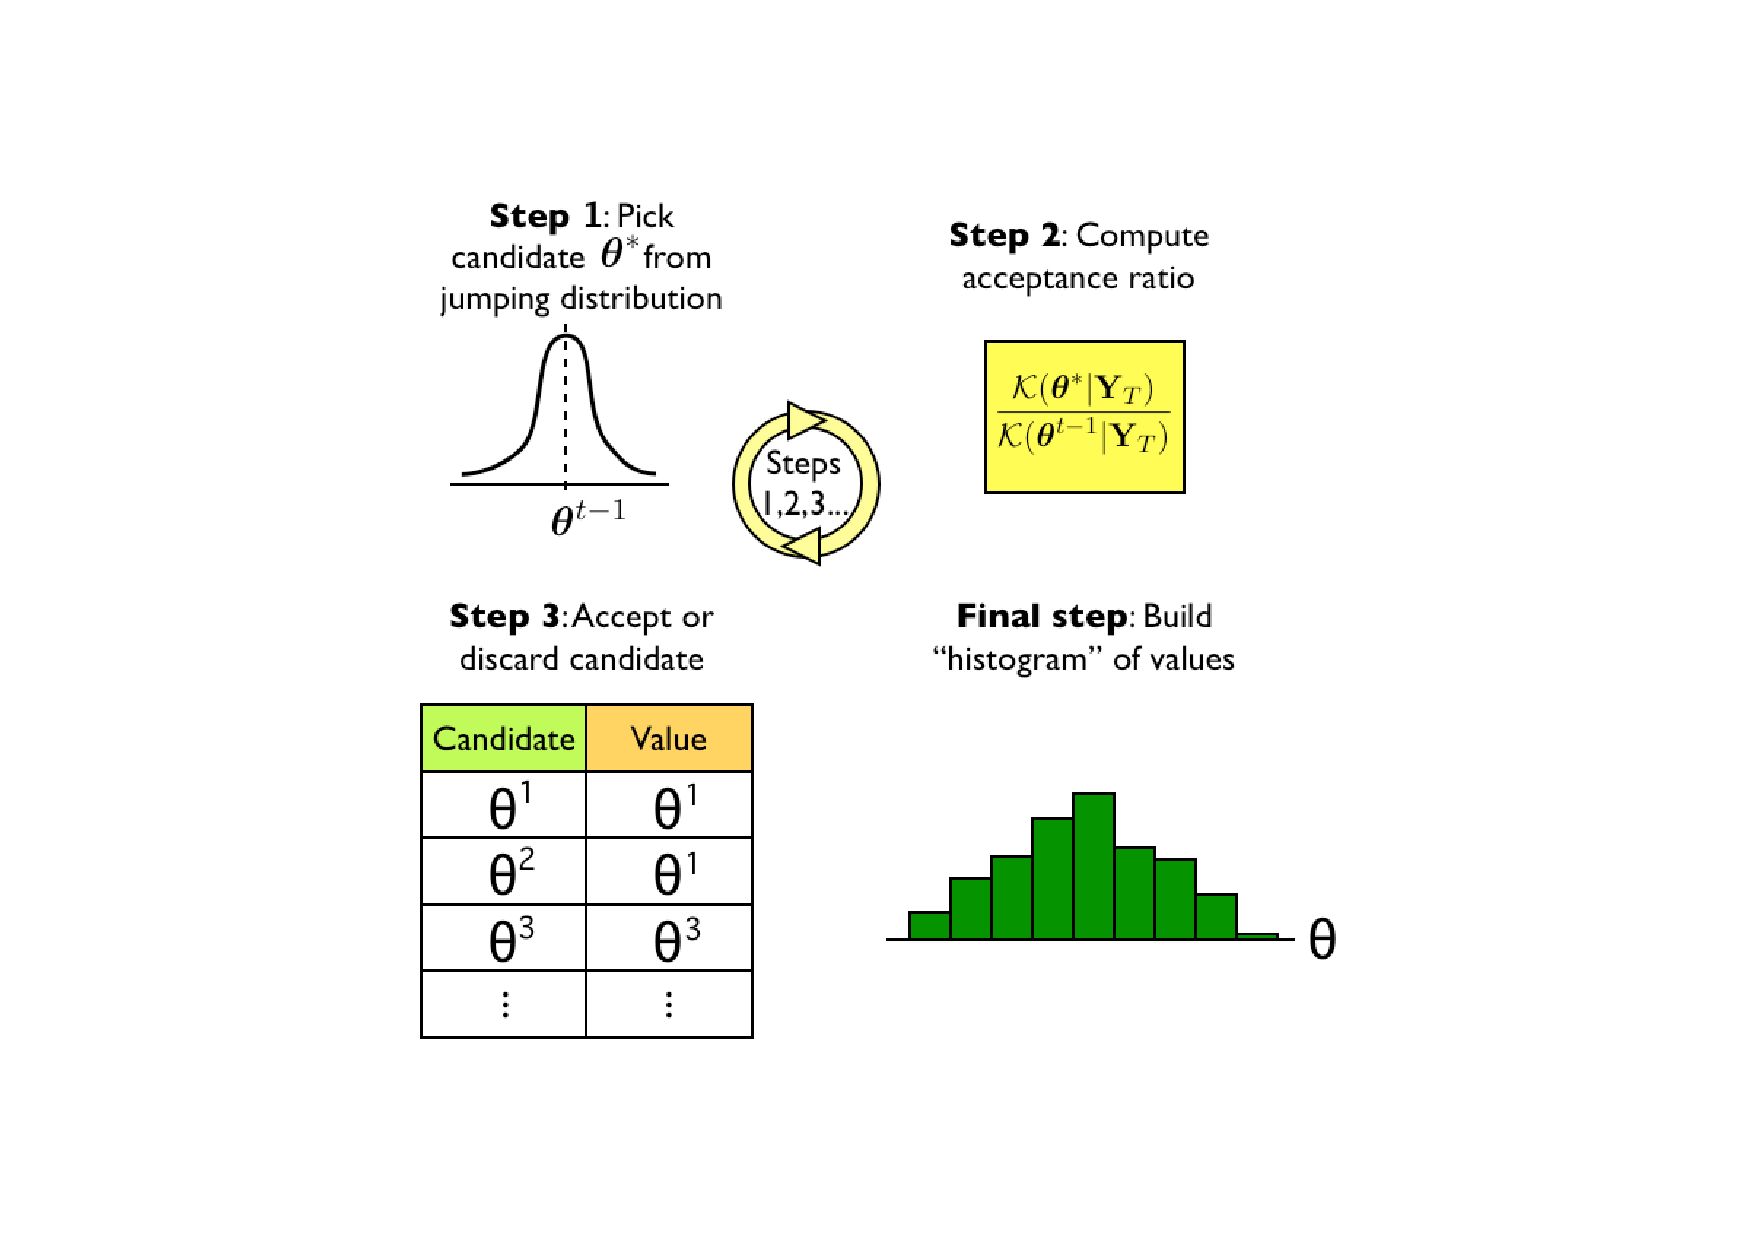
\includegraphics[width=1.0\textwidth]{P_MH2} 
\end{center} 
\caption[Illustration of the Metropolis-Hastings algorithm]{The above sketches the Metropolis-Hastings algorithm, used to build the posterior distribution function. Imagine repeating these steps a large number of times, and smoothing the ``histogram'' such that each ``bucket'' has infinitely small width.} 
\end{figure}

But why have such a complicated acceptance rule? The point is to be able to visit the entire domain of the posterior distribution. We should not be too quick to simply throw out the candidate giving a lower value of the posterior kernel, just in case using that candidate for the mean of the drawing distribution allows us to to leave a local maximum and travel towards the global maximum. Metaphorically, the idea is to allow the search to turn away from taking a small step up, and instead take a few small steps down in the hope of being able to take a big step up in the near future. Of course, an important parameter in this searching procedure is the variance of the jumping distribution and in particular the \textbf{scale factor}. If the scale factor is too small, the \textbf{acceptance rate} (the fraction of candidate parameters that are accepted in a window of time) will be too high and the Markov Chain of candidate parameters will ``mix slowly'', meaning that the distribution will take a long time to converge to the posterior distribution since the chain is likely to get ``stuck'' around a local maximum. On the other hand, if the scale factor is too large, the acceptance rate will be very low (as the candidates are likely to land in regions of low probability density) and the chain will spend too much time in the tails of the posterior distribution. \\

While these steps are mathematically clear, at least to a machine needing to undertake the above calculations, several practical questions arise when carrying out Bayesian estimation. These include: How should we choose the scale factor $c$ (variance of the jumping
        distribution)? What is a satisfactory acceptance rate? How many draws are ideal? How is convergence of the Metropolis-Hastings iterations assessed? These are all important questions that will come up in your usage of Dynare. They are addressed as clearly as possible in section \ref{sec:estimate} of Chapter \ref{ch:estbase}. \\

\section{Comparing models using posterior distributions}
As mentioned earlier, while touting the advantages of Bayesian estimation, the posterior distribution offers a particularly natural method of comparing models. Let's look at an illustration. \\

Suppose we have a prior distribution over two competing models: $p(\mathcal{A})$ and $p(\mathcal{B})$. Using Bayes' rule, we can compute the posterior
            distribution over models, where $\mathcal{I}=\mathcal{A},\mathcal{B}$ 
        \[
            p(\mathcal{I}|\mathbf Y_T) = \frac{p(\mathcal{I})p(\mathbf Y_T|\mathcal{I})}
            {\sum_{\mathcal{I}=\mathcal{A},\mathcal{B}}p(\mathcal{I})p(\mathbf Y_T|\mathcal{I})}
        \]
where this formula may easily be generalized to a collection of $N$ models.

Then, the comparison of the two models is done very naturally through the ratio of the posterior model distributions. We call this the \textbf{posterior odds ratio}:
        \[
            \frac{p(\mathcal{A}|\mathbf Y_T)}{p(\mathcal{B}|\mathbf
            Y_T)} = \frac{p(\mathcal{A})}{p(\mathcal{B})}
            \frac{p(\mathbf Y_T|\mathcal{A})}{p(\mathbf Y_T|\mathcal{B})}
        \]

The only complication is finding the magrinal density of the data conditional on the model, $p(\mathbf Y_T|\mathcal{I})$, which is also the denominator of the posterior density $p(\boldsymbol\theta | \mathbf Y_T)$ discussed earlier. This requires some detailed explanations of their own. \\

For each model $\mathcal{I}=\mathcal{A},\mathcal{B}$ we can evaluate, at least theoretically, the marginal
        density of the data conditional on the model by integrating out the deep parameters $\boldsymbol\theta_{\mathcal{I}}$ from the posterior kernel:
        \[
            p(\mathbf Y_T|\mathcal{I}) = \int_{\Theta_{\mathcal{I}}} p(\boldsymbol\theta_{\mathcal{I}}; \mathbf Y_T
            |\boldsymbol\theta_{\mathcal{I}},\mathcal{I}) d\boldsymbol\theta_{\mathcal{I}} = \int_{\Theta_{\mathcal{I}}} p(\boldsymbol\theta_{\mathcal{I}}|\mathcal{I})\times p(\mathbf Y_T
            |\boldsymbol\theta_{\mathcal{I}},\mathcal{I}) d\boldsymbol\theta_{\mathcal{I}}
        \]
Note that the expression inside the integral sign is exactly the posterior kernel. To remind you of this, you may want to glance back at the first subsection above, specifying the basic mechanics of Bayesian estimation.\\
        
        To obtain the marginal density of the data conditional on the model, there are two options. The first is to assume a functional form of the posterior kernel that we can integrate. The most straightforward and the best approximation, especially for large samples, is the Gaussian (called a \textbf{Laplace approximation}). In this case, we would have the following estimator:
\[
\widehat{p}(\mathbf Y_T|\mathcal I) = (2\pi)^{\frac{k}{2}}|\Sigma_{\boldsymbol\theta^m_{\mathcal I}}|^{\frac{1}{2}}p(\boldsymbol\theta_{\mathcal I}^m|\mathbf
Y_T,\mathcal I)p(\boldsymbol\theta_{\mathcal I}^m|\mathcal I)
\]
where $\boldsymbol\theta_{\mathcal I}^m$ is the posterior mode. The advantage of this technique is its computational efficiency: time consuming Metropolis-Hastings iterations are not necessary, only the numerically calculated posterior mode is required. \\

The second option is instead to use information from the Metropolis-Hastings runs and is typically referred to as the \textbf{Harmonic Mean Estimator}. The idea is to simulate the marginal density of interest and to simply take an average of these simulated values. To start, note that
\[
p(\mathbf{Y}_T|\mathcal I)=\mathbb{E}\left[\frac{f(\boldsymbol\theta_{\mathcal I})}{p(\boldsymbol\theta_{\mathcal I}|\mathcal I)
            p(\mathbf{Y}_T|\boldsymbol\theta_{\mathcal I},\mathcal I)}\biggl|\boldsymbol\theta_{\mathcal I},\mathcal I\biggr.\right]^{-1}
\]
where $f$ is a probability density function, since 
\[
                \mathbb{E}\left[\frac{f(\boldsymbol\theta_{\mathcal I})}{p(\boldsymbol\theta_{\mathcal I}|\mathcal I)
                p(\mathbf{Y}_T|\boldsymbol\theta_{\mathcal I},\mathcal I)}\biggl|\boldsymbol\theta_{\mathcal I},\mathcal I\biggr.\right]
                =
                \frac{\int_{\Theta_{\mathcal I}}f(\boldsymbol\theta)d\boldsymbol\theta}{\int_{\Theta_{\mathcal I}}p(\boldsymbol\theta_{\mathcal I}|I)
                p(\mathbf{Y}_T|\boldsymbol\theta_{\mathcal I},\mathcal I)d\boldsymbol\theta_{\mathcal I}}
\]
and the numerator integrates out to one (see\citet{Geweke1999} for more details). \\

This suggests the following estimator of the marginal
        density
        \[
            \widehat{p}(\mathbf{Y}_T|\mathcal I)= \left[\frac{1}{B}\sum_{b=1}^B
            \frac{f(\boldsymbol\theta_{\mathcal I}^{(b)})}{p(\boldsymbol\theta_{\mathcal I}^{(b)}|\mathcal I)
            p(\mathbf{Y}_T|\boldsymbol\theta_{\mathcal I}^{(b)},\mathcal I)}\right]^{-1}
        \]
where each drawn vector $\boldsymbol\theta_{\mathcal I}^{(b)}$ comes from the
        Metropolis-Hastings iterations and where the probability density function $f$ can be viewed as a weights on the posterior kernel in order to downplay the importance of extreme values of $\boldsymbol\theta$. \citet{Geweke1999} suggests to use a truncated Gaussian function, leading to what is typically referred to as the \textbf{Modified Harmonic Mean Estimator}. \\    
            
            

\chapter{Optimal policy under commitment} \label{ch:ramsey}
\chapter{Troubleshooting} \label{ch:trouble}

To make sure this section is as user friendly as possible, the best is to compile what users have to say! Please let me know what your most common problem is with Dynare, how Dynare tells you about it and how you solve it. Thanks for your precious help!

\backmatter

\bibliography{DynareBib}
\bibliographystyle{econometrica}
%\printindex

\end{document}

